% Paper size, fontstyle, normal fontsize----------------------------------------
\documentclass[a4paper,12pt]{article}
\usepackage[magyar]{babel}
\usepackage{t1enc}% ékezetes szavak automatikus elválasztásához
%\usepackage{times}
\usepackage{mathptmx}
\usepackage{caption}
\usepackage{enumitem}
\usepackage{parskip}
\usepackage[utf8]{inputenc}
\usepackage{url}
\pagenumbering{arabic} 
\usepackage[linktoc=none]{hyperref}
\usepackage{url}
\usepackage{amsmath}
\usepackage{setspace}
\usepackage{framed} % Framing content
\usepackage{multicol} % Multiple columns environment
\usepackage{nomencl}
\makenomenclature
\renewcommand{\nomname}{Nevezéktan}

% Fontsize subection,section----------------------------------------------------

\usepackage{titlesec}
% Set section font settings
\titleformat{\section}
{\normalfont\fontsize{14}{16}\bfseries}{\thesection}{1em}{}

% Set subsection font settings
\titleformat{\subsection}
{\normalfont\fontsize{12}{14}\bfseries}{\thesubsection}{1em}{}
% Set subsection spacing settings
%\titlespacing{\subsection}{0pt}{1\baselineskip}{1\baselineskip}

% Set text font settings
\renewcommand{\normalsize}{\fontsize{12}{14}\selectfont}

% Sorkoz
\setstretch{1.15}


% Linebreaks after figures and lists----------------------------------------------

% Automatically insert line break after figures
\captionsetup[figure]{position=below}

% Automatically insert line break after lists
%\setlist[itemize]{after=\vspace{\baselineskip}}

% Margins-------------------------------------------------------------------------

\usepackage{geometry}
\geometry{
	left=25mm,
	right=25mm,
	top=25mm,
	bottom=40mm
}

% Justify text--------------------------------------------------------------------

\usepackage{ragged2e}

% --------------------------------------------------------------------------------

\usepackage[skins,theorems]{tcolorbox}
\usepackage{multicol}
\usepackage{listings}
\usepackage{color}
\usepackage{multirow}
\usepackage{graphicx}
\usepackage{subfig}
\usepackage{bm}
\usepackage{matlab-prettifier}

\definecolor{dkgreen}{rgb}{0,0.6,0}
\definecolor{gray}{rgb}{0.5,0.5,0.5}
\definecolor{mauve}{rgb}{0.58,0,0.82}

\lstset{frame=tb,
	style=Matlab-editor,
	aboveskip=3mm,
	belowskip=3mm,
	showstringspaces=false,
	columns=flexible,
	basicstyle={\small\ttfamily},
	numbers=none,
	numberstyle=\tiny\color{gray},
	keywordstyle=\color{blue},
	commentstyle=\color{dkgreen},
	stringstyle=\color{mauve},
	breaklines=true,
	breakatwhitespace=true,
	tabsize=3
}
\newcommand\Pbracket[1]{\left(#1\right)}
\newcommand\tab[1][1cm]{\hspace*{#1}}
\DeclareUnicodeCharacter{2212}{\textendash}

\title{ 
	Szakdolgozat
	\linebreak
	Három - fázisú aszinkron gép mezőorientált szabályozása}
\author{Arnóczy László}
\date{2022.11.24}

\begin{document}
		
	\section*{Absztrakt}
	A szakdolgozat célja egy olyan szabályozási kör tervezése, mely alkalmas aszinkron gép nyomatékszabályozásának megvalósítására. A szabályozás a motor állórészéhez tartozó mágneses mező megfelelő gerjesztésén alapul, melyet a teljesítmény elektronika megfelelő irányításával, valamint a motorról szükséges mérések visszacsatolásával tudunk szabályozni. A motor folyamatos forgatása mellet, a tranziens állapotok lecsengésével, az indukciós gép nyomatéka a referencia nyomatékhoz közeli értékben fog állandósulni.
	\pagebreak
	
	\section*{Abstract}
	The main purpose of this thesis is to design a control loop, which is suitable for torque control of asynchronous machine. The control mechanism relies on the appropriate excitation of the magnetic field associated with the stator, which can be regulated by the proper control of power electronics and the necessary feedback measurements of the motor. While the motor is continuously rotating, after the transient states, the torque of the induction machine will be stabilized close to the reference torque.
	\pagebreak
	
	\tableofcontents
	\pagebreak
	
	\justifying
	
	\section{Bevezetés}
	
	Napjainkban az autók általi károsanyag-kibocsátás minimalizálása kulcsfontosságú téma mind az ember és a környezet tekintetében. A légszennyezés jelentős része, a fosszilis-üzemanyaggal működő belső égésű motorokat használó autókra esik. Az elektromos autók mind a jelenben, mind a jövőben egy alternatívát biztosítanak az autóvásárlás tekintetében. Az elektromos autók fejlesztése rengeteg innovációt követel meg a hajtáslánc minden komponensének tekintetében. Témám fókusza ezen innovációk közül a hajtásvezérlések témakörébe esik. Teljesítmény elektronika oldalról a többszintű inverterek, számítási teljesítmény terén pedig a mikrokontrollerek/fpga-ak megjelenése jelentősen mértékben elősegítette többfázisú motorok valós idejű, pontosabb vezérlését. A gyorsabb beavatkozás lehetővé tette bonyolultabb logikájú szabályozási körök implementálást. A hajtás szoftveres komponenseinek fordítását az EDU (Electrical Drive Unit) végzi. Ez a vezérlő csak a motor szabályozáshoz közvetlenül kapcsolódó számításokkal foglalkozik (például: referencia áram számolás). A hajtásszabályozásokat két nagy csoportra tudjuk osztani: skalár kontroll és vektor kontrol. A vektor kontrollok közül két fő típust tudunk megkülönböztetni: közvetlen nyomaték szabályozás (Direct torque control), valamint a mezőrorientált szabályozás (Field-oriented control). Mindkét technika a zárt kör szabályozásán alapul. Ezen hajtásszabályozások a DC motor elvén valósulnak meg, ennek megfelelően a megfelelő koordináta transzformációkat alkalmazva az áramokat, fluxusokat, feszültségeket fluxus és nyomatékképző komponensekre osztjuk, a koordináta rendszert pedig úgy orientáljuk, hogy a rotorfluxus vektor megegyezzen a koordináta rendszer fluxusképző komponensének irányával, tehát a rotorfluxus vektor nyomatékképző komponense 0 legyen. Ezen feltételek lehetővé teszik több fázisú motorok irányítását. A motorválasztás tekintetében az elektromos autókban használt motorok két nagy csoportra oszthatók: állandó mágneses szinkron gép (Permanent magnet synchronous machine) vagy aszinkron gép (Induction machine). Szakdolgozatomban aszinkron gépre tervezett mezőorientált szabályozást fogok bemutatni szimulációs környezetben MATLAB Simulink használatával, amely tartalmazza a szükséges szoftveres és hardveres elemeket és optimális energiahatékonyság mellet képes a motort adott nyomaték referenciára szabályozni. A szabályozás alapja az  állórész mágneses mezőjének megfelelő gerjesztése. Ennek megfelelően a nyomatékszabályozáshoz szükséges visszacsatolt értékeket az állórész D-Q állókoordináta rendszerbe transzformált áramai, valamint a rotorfluxus szög képezi. Teljesítmény elektronikát tekintve a motor táplálását egy két szintű három fázisú inverter biztosítja. A hardveres komponenseket elemezve a mikrokontroller a vezérlőszervnek, az inverter a beavatkozószervnek, a motor pedig az irányított szakasznak feleltethető meg. A szimuláció tranziens állapotának lecsengésével a motor állapota a terhelőgépnek beállított szögsebesség, valamint a referencia nyomaték tekintetében fog állandósulni. A hardveres Simscape és szoftveres Simulinkes elemeket tartalmazó szimuláció tesztelés után alkalmassá válik a kódgenerálásra, amely implementálható mikrokontrollerre. A kód implementálása után, és a megfelelő hardveres megvalósítást követően lehetőségünk van valós környezetben tesztpadon működtetni a rendszert, mely során a méréseket elemezve komplex képet kaphatunk a szabályozásunk hatásfokáról és esetleges tovább fejlesztési lehetőségeiről.

	
	\pagebreak
	\section {Mezőorientált szabályozás elvi felépítése és bemutatása}
	
		\begin{figure}[!htb]
			\centering
			\label{fig:Control séma}
			\tcbox{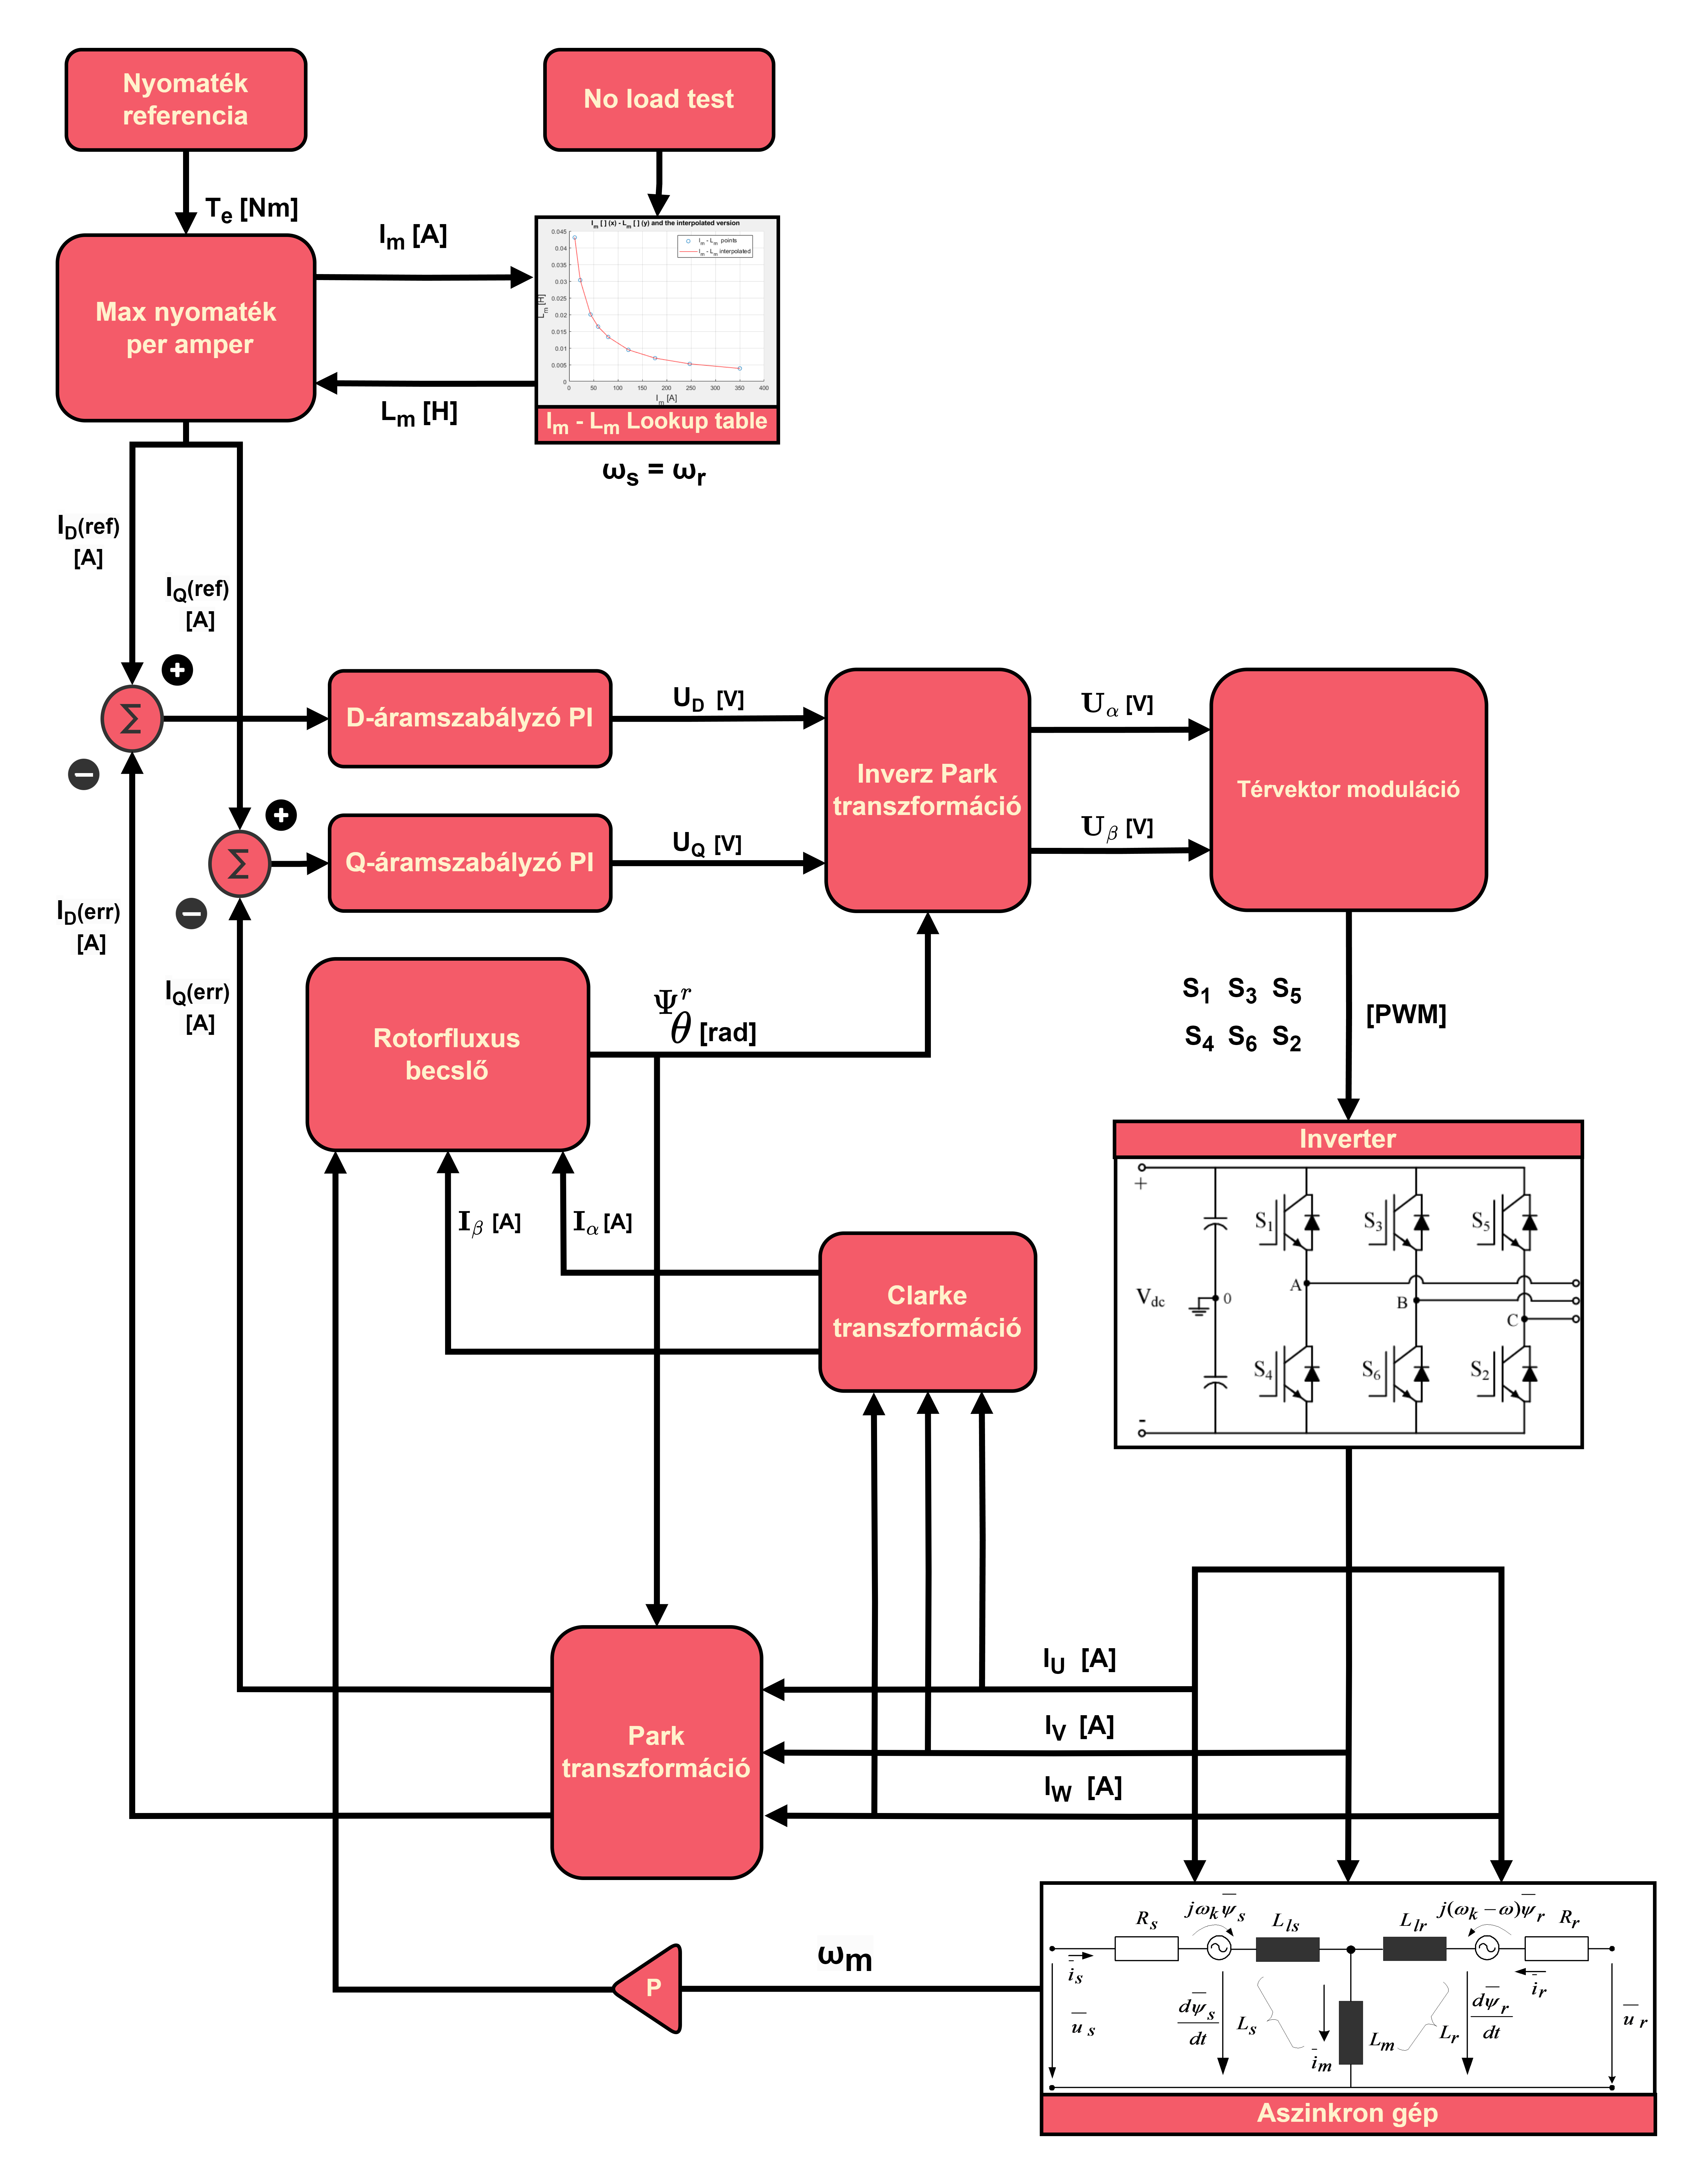
\includegraphics[width=15cm]{ControlScheme}}
			\caption{Megvalósított mezőorientált szabályozás felépítése }		
		\end{figure}
		
	\pagebreak
	Manapság többfázisú szinkron és aszinkron gépek tekintetében a mezőorientált szabályozás (Field-oriented control) tekinthető a leghatékonyabb motorvezérlésnek. Ennek a szabályozási módnak a megjelenése jelentős mértékben növelte a motorok teljesítményének kihasználását, a korábban használt skalár kontrollokhoz képest. Mind nyomaték és sebességszabályozásra is alkalmas. Megjelenése 1970 körülire tehető. A szabályozás vektor kontrollnak tekinthető, mely alapját a motor áramainak fluxus és nyomatékképző komponensre történő bontása, valamint a rotorfluxus szög visszacsatolása képezi. Emellett a D-Q koordináta rendszert úgy orientáljuk, hogy a rotorfluxus vektor Q-irányú komponense nulla legyen, tehát megegyezzen a D-iránnyal. Ezen feltételek teljesítésében a koordináta transzformációk jelentős szereppel bírnak (Clarke és Park transzformáció), ezek nélkül nem lenne megvalósítható a szabályzó kör. Szakdolgozatomban a mezőorientált szabályozás egy nyomatékszabályzást valósít meg, amely számba veszi a főmező induktivitás szaturációját. A nyomatékszabályozás áramszabályozásként valósítható meg, melynek referencia jeleit a legkisebb áramokat szolgáltató MTPA (Maximum nyomaték per amper) stratégia számolja ki. Az MTPA egy adott terhelő szögsebesség és nyomaték referenciára kiszámolja az adott nyomatékhoz tartozó legkisebb áramokat, amelyek az adott nyomaték előállításához szükségesek. Az áramszabályzók diszkrét idejű PI szabályzók anti-wind up technikával. Az áramszabályzók kimenetei az Inverz Park transzformáció után, az invertervezérlés bemeneti lesznek, dimenziójukban feszültségeknek tekinthetőek. Az inverter vezérlést SVPWM-el (Space vector pulse width modulation) technikával valósítottam meg, mely optimális kapcsolási mintával képezi le a megfelelő fázisfeszültségeket. Emellett hatékonyságban sokkal optimálisabban használja ki a DC feszültséget, mint egy sima szinuszos moduláció, ez a fázisfeszültségek maximális amplitúdójának nagyságából látható. A motor mágneses mezőjének visszacsatolására, egy áramalapú rotorfluxus becslőt implementáltam, amely resolver használata mellett kellő pontossággal határozza meg a visszacsatolást képező rotorfluxus szöget.
	\pagebreak
	\section{Aszinkron gép helyettesítő áramköre és egyenletei }
	
	Az aszinkron gép felépítésében egy transzformátorra hasonlít, ahol a szekunder tekercs forog. A primer oldalt az állórész háromfázisú tekercselése, a szekunder tekercset pedig a rotor oldal képezi. Ahhoz, hogy a rendszer szimmetrikus legyen, az állórész tekercselése fázisonként 120 $^{\circ}$-ban tér el egymástól. Az irodalomban sokszor "induction machine" néven hivatkoznak rá, ugyanis működése az indukció elvén alapul. A fizikát alapul véve a motor működése a Faraday-féle indukciós törvény, és a Lenz-törvényen alapszik. Az indukciós törvény kimondja, mely szerint az időben változó mágneses mező feszültséget indukál, melyet a fluxus változás nagysága határoz meg. A Lenz-törvény értelmében az indukált feszültség iránya pedig ellentétes lesz a fluxus változással. Az állórész tekercselése váltakozó áram hatására feszültséget indukál a forgórészben. Mivel a forgórész rövidre van zárva, áram jön létre a rotorban, amely szintén mágneses mezőt hoz létre. Az indukált áram által létrehozott mágneses mező és az állórész forgó mágneses mezője közötti kölcsönhatás, azaz a mágneses erővonalak metszése hozza létre a forgórész forgónyomatékát.
	\begin{align}
		& U_i = -\frac{d \Psi}{dt}
	\end{align}
	Ahhoz, hogy a forgórész forgatónyomaték kialakuljon, a két rész mágneses mezőjének sebessége nem lehet ugyanakkora, ugyanis ebben az esetben a mágneses erővonalak egybeesnének, nem metszenék egymást. Az állórész és a forgórész mágneses mezőjének szögsebessége közötti eltérést slip-nek nevezzük, az aszinkron gép elnevezés ebből adódik.
	\begin{align}
		& \omega_{slip} = \omega - \omega_{r}
	\end{align}
	A két transzformátoros D-Q helyettesítő képleteket úgy kapjuk, hogy a motor áramait felosztjuk fluxus és nyomatékképző komponensekre, ezt a Clarke és Park-transzformáció alkalmazásával tudjuk megtenni. A D-irányt a fluxusképző komponensnek, a Q-irányt a nyomatékképző komponensnek tekintjük. Ilyenkor a háromfázisú álló koordináta-rendszerből, egy kétfázisú forgó koordináta-rendszerbe képezünk le, amely a szinkron szögsebességgel forog. A Clarke-transzformációt a térvektor modulációnál, a Park transzformációt rotorfluxus becslő bemutatásánál fogom részletezni. 

	\subsection{Feszültség egyenletek}
	
	A transzformáció során kapott feszültség egyenletekből jól látszik, hogy a feszültséget az adott oldal ellenállása, fluxus időbeli változása, az adott oldal szögsebessége és a fluxus aktuális értékének szorzata határozza meg. Emellett az is látszik, hogy a rotor oldalt a stator oldalról nézve az a slip sebességgel forog. Állandósult állapotban mind a rotor, mind a stator oldali egyenletekben a fluxusváltozás nullának tekinthető.
	\begin{align}
		& V_{qs} = R_{s} i_{qs} + \frac{d \Psi_{qs}}{dt} + \omega \Psi_{ds} & V_{qr} = R_{r} i_{qr} + \frac{d \Psi_{qr}}{dt} + (\omega - \omega_{r}) \Psi_{dr} \\
		& V_{ds} = R_{s} i_{ds} + \frac{d \Psi_{ds}}{dt} - \omega \Psi_{qs} & V_{dr} = R_{r} i_{dr} + \frac{d \Psi_{dr}}{dt} - (\omega - \omega_{r}) \Psi_{dr}				
	\end{align}
	
	\subsection{Fluxus és induktivitás egyenletek}
	
	A fluxust az tekercsen átfolyó áram és annak induktivitásának szorzata adja. Az egyenletekből jól látható, hogy a főmező induktivitáson mindkét oldalról folyik áram, a forgórész kölcsönös indukciója miatt. A motor felépítését tekintve, a tekercsek egyes részein az elhelyezkedésükből adódóan olyan fluxus is generálódik, amelynek mágneses erővonalai nem metszik a másik oldal mezőjét, a tekercs ezen részeit szórási induktivitásoknak nevezzük. ($L_{ls}$,$L_{lr}$).
	\begin{align}
		& \Psi_{qs} = L_{s} i_{qs} + L_{m} i_{qr} & \Psi_{qr} = L_{r} i_{qr} + L_{m} i_{qs} \\
		& \Psi_{ds} = L_{s} i_{ds} + L_{m} i_{dr} & \Psi_{dr} = L_{r} i_{dr} + L_{m} i_{ds} \\
		& L_{s} = L_{ls} + L_{m} & L_{r} = L_{lr} + L_{m} &
	\end{align}
	
	\subsection{Nyomaték egyenletek}
	
	\begin{align}
		& Te = \frac{3}{2} \cdot p \cdot \frac{{L_m}^2}{L_r} \cdot i_{ds} \cdot i_{qs}  
		& Te = \frac{3}{2} \cdot p \cdot (\Psi_{ds} \cdot i_{qs} - \Psi_{qs} \cdot i_{ds} )
	\end{align}
	
	\begin{figure}[!htb]
		\centering
		\label{fig:Async}
		\tcbox{\includegraphics[width=8cm]{Async}}
		\caption{Aszinkron gép D-Q helyettesítő áramkörei}		
	\end{figure}
	\pagebreak
	
	\section {Maximum nyomaték per amper stratégia tervezése}
	
		\subsection{Komponens célja}
		
		A maximális nyomaték per amper (MTPA) egy olyan vezérlési stratégia, amely optimalizálja a motor nyomatékát az áramfelvételhez képest. Az aszinkron gép adott nyomaték karakterisztikáját ábrázolva az állórész D-Q áramainak koordináta-rendszerében ($ x = i_{sd} , y = i_{sq}$) egy nyomatékgörbét kapunk. Ebből következik, hogy különböző D-Q áram kombinációk hatására ugyanazon nyomaték mérhető a motoron. Ha vektort képzünk ezekből az áram párokból, nagyságuk eltérő lesz. Célunk, hogy megtaláljuk azt a D-Q áram párt, amely a legkisebb áramerősség mellett képes a referencia nyomaték előállítására. Ezzel növeljük a motor hatásfokát, valamint az áramtól négyzetesen függő veszteségeket ($I^2t$) is minimalizáljuk. Az áramszabályzók referencia jelei ezen értékek lesznek. Nyomatékszabályozásnál a terhelőgép adott szögsebességre terhel. Ez a sebesség megegyezik a rotor mechanikai szögsebességével.
		 
		\subsection {D - Q áramok meghatározása}
		
		A nyomatékgörbék meghatározásához szükséges megadni az áramvektor és a szögének maximális értékét, majd egy adott áram, és szög lépésközzel különböző áramvektorokat képezve, a vektor D és Q - irányú komponensét. Ennek eredményeképpen minél kisebb a lépésköz annál több fajta D - Q árampárt tudunk megvizsgálni, hogy az általuk előállított nyomaték megfelel-e a referenciának. Az áramvektor maximális értéke a motor fizikai paramétereiből számolható, a maximális szög paraméternek tekinthető, értéke $ \frac{\pi}{2}$. Trigonometrikus azonosságokat használva az áramvektort Descartes-koordináta rendszerben ábrázolva, az x-irány adja a D-irányú komponenst, y-irány pedig a Q-irányú komponenst. Ez alapján a D-Q áramokat az alábbi módon határozzuk meg:
		\begin{align}
			& i_{ds} = |\vec{I}_s| \cdot cos (\Theta) \\
			& i_{qs} = |\vec{I}|_s \cdot sin (\Theta)
		\end{align}
		
		\subsection{Mágneses telítődés és NO LOAD teszt}
			
			Az indukciós gép forgórésze egy ferromágneses anyag. Az állórész vasmagos tekercsei által generált elektromágneses tér hatására a forgórészben indukált feszültség keletkezik, ami áramot hoz létre a forgórészben. Tehát aszinkron gépnél az állórész tekercseinek fluxusa alakítja mágnessé a forgórészt. Az áram nagyságát növelve a vasmagos tekercsek induktivitása nem lineárisan csökken. Ezt a jelenséget a főmező induktivitás mágneses telítődéseként azonosítjuk. A No - load teszt lényege, hogy a motor mágneses szaturációs paramétereiből (áram - vonali feszültség táblázat), valamint az ismert motorparaméterek felhasználásával kiszámoljuk mekkora főmező induktivitás mérhető a stator körben, miközben a rotor szögsebessége megegyezik szinkron sebességgel, ezáltal csak a stator körben folyik áram ($i_{r} = 0$), ugyanis az álló és forgórész mágneses erővonalai egybeesnek. Az áram szögsebessége a motor nominális (mezőgyengítési ponthoz tartozó) frekvenciájából számolható. Ennek eredményeképpen egy mágnesező áram [A] - főmező induktivitás [H] táblázatot kapunk.
			
			\begin{figure}[!htb]
				\centering
				\label{fig:Async}
				\tcbox{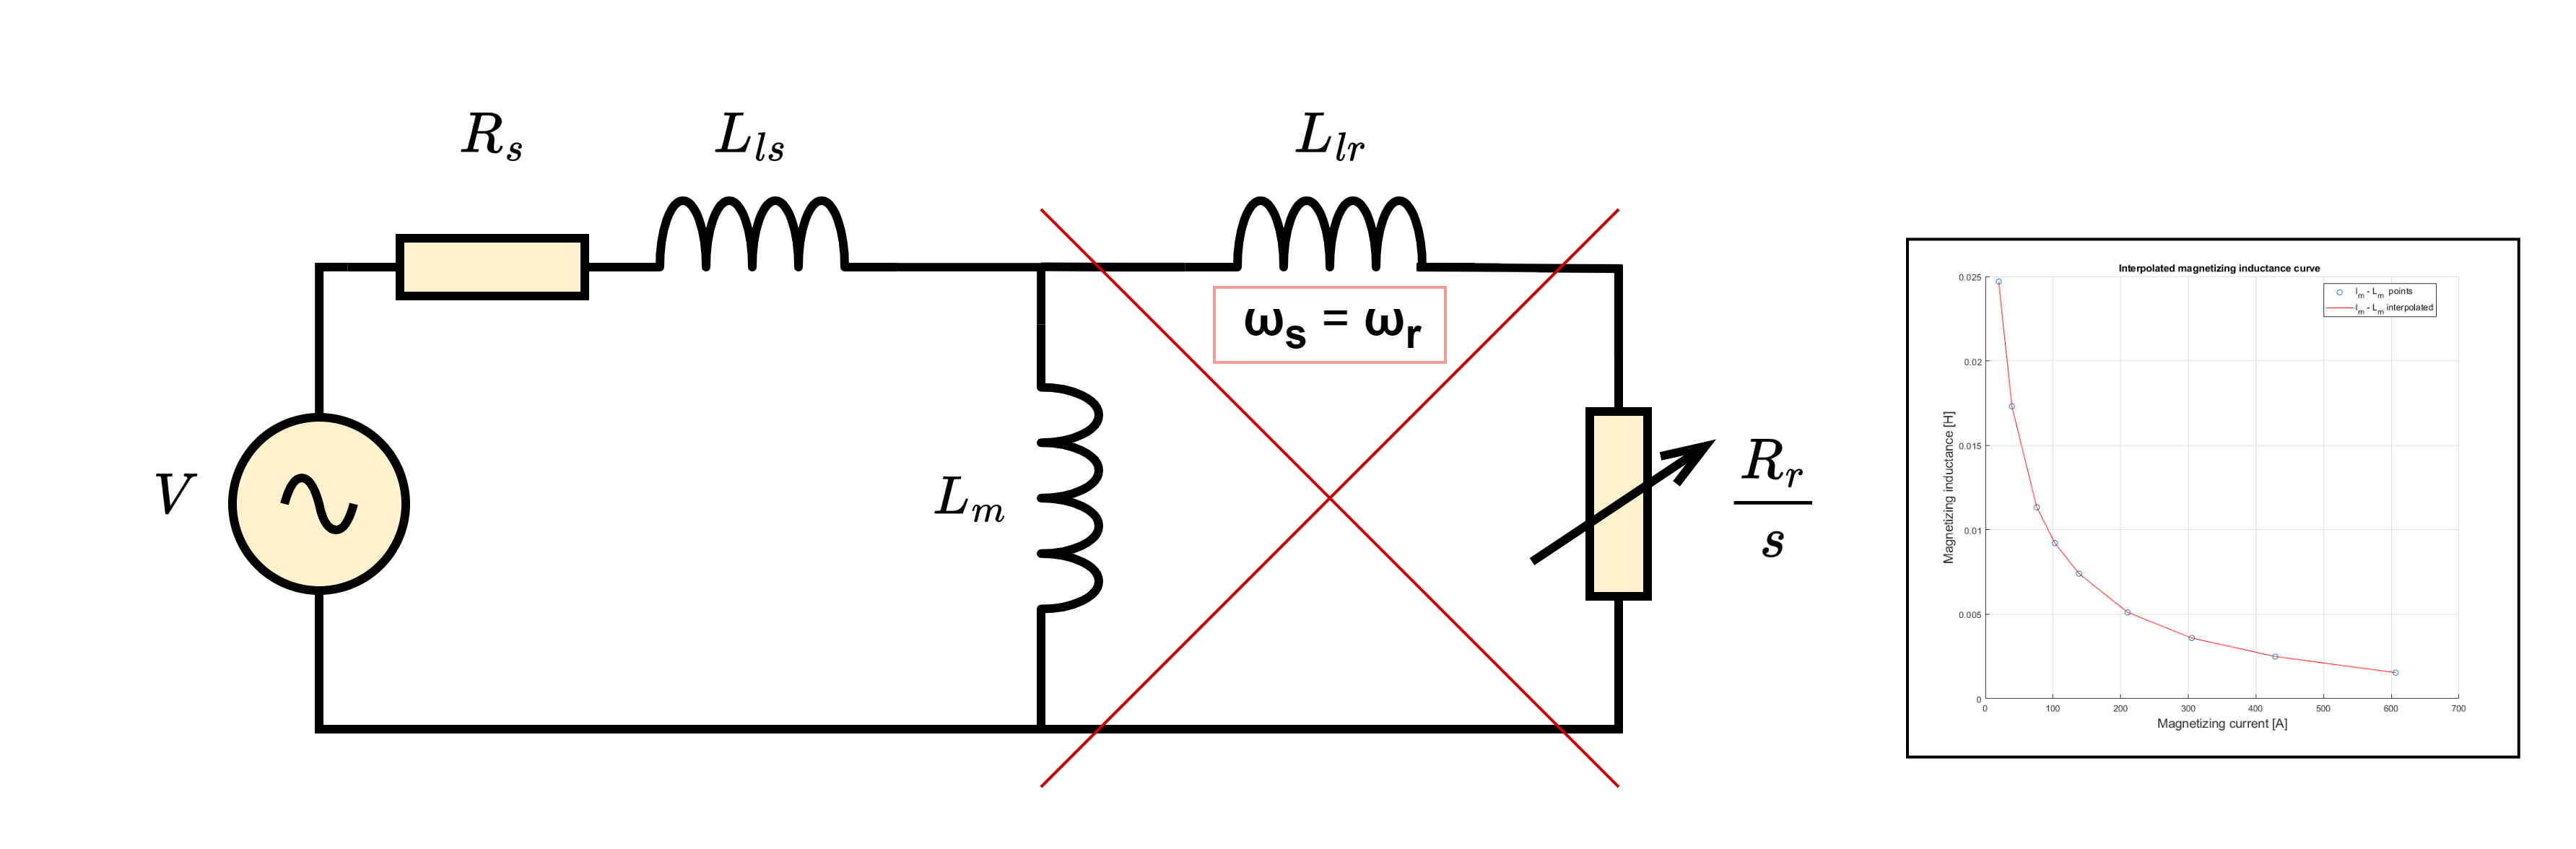
\includegraphics[width=15cm]{NoLoad2}}
				\caption{NO-LOAD teszt kapcsolási rajza és főmező induktivitás mágneses telítődése }		
			\end{figure}
			A főmező induktivitás értékét egy egyszerű impedancia számításból kapjuk.
			\begin{align}
				& Z = \sqrt{ R_s^2 + X_{L}^2}= \frac{U}{I} & L_{m} = \sqrt\frac{(U/I)^2 -R_s^2}{\omega_{rated}} - L_{Ls}
			\end{align}
		
		\subsection{Mágnesező áram nagyságának meghatározása }
		
			A főmező induktivitás és slip meghatározásához szükséges a mágnesező áram kiszámolása. Mágnesező áram a főmező induktivitáson átfolyó áramot jelenti. Ehhez szükséges a rotor oldali áramok meghatározása. Mezőorientált szabályozásban a D - Q koordináta rendszert úgy orientáljuk, hogy a rotorfluxus vektor megegyezzen a koordináta rendszer fluxus képző irányával, tehát a rotorfluxus nyomatékképző komponense 0 ($\Psi_{qr} = 0$).
			
			Mágnesező áram meghatározása:
			\begin{align}
				& i_{qr} = - \frac{L_m \cdot i_{qs}}{L_r} \\
				& \Psi_{qs} = L_s \cdot i_{qs} + L_m \cdot i_{qr} \\
				& \Psi_{ds} = \frac{Te}{\frac{3}{2} \cdot p } + \frac{\Psi_{qs} \cdot i_{ds}}{i_{qs}} \\
				& i_{dr} = \frac{\Psi_{ds} - (L_s \cdot i_{ds} ) }{L_{m}} \\
				& \vec{i}_{m} =  (i_{ds} + i_{dr}) + i \cdot (i_{qs} + i_{qr})  \\
				& |\vec{i}_{m}| = \sqrt{(i_{ds} + i_{dr})^2 + (i_{qs} + i_{qr})^2}
			\end{align}
			
		\subsection{Főmező induktivitás meghatározása iteratív módon  }	
		
			Az első iterációban egy kezdeti $ L_m $ értékkel kiszámoljuk mekkora mágnesező áramot eredményez, majd a meghatározzuk a hozzátartozó induktivitás értékét, az üresjárási mérés interpolált függvényéből.
			
			\begin{itemize}
				\item Ha a mágnesező áram kisebb mint a legkisebb áram érték az $i_m$ - $L_m$ look-up table-ben, akkor a legelső $L_m $ értéket választjuk.
				\item Ha a mágnesező áram nagyobb mint a legnagyobb áram  érték az $i_m$ - $L_m$ look-up table-ben, akkor a legutolsó $L_m $ értéket választjuk. 
				\item Ha a fentiek nem igazak, akkor interpoláció segítségével keressük ki a megfelelő értéket
			\end{itemize}
			
			A következő iterációban a visszaszámolt érték $L_m [k-1]$ lesz, majd elvégezzük újra fentebbi lépéseket, amiből megkapjuk az aktuális $L_m [k]$ értéket. A két érték közötti relatív tolerancia számításából, meghatározzuk hogy a két érték közötti eltérés elhanyagolható-e. Ha igen, akkor a továbbiakban ezt az $ L_m $ értéket fogjuk használni. A számolt nyomaték, és referencia nyomaték közötti tolerancia vizsgálat, ugyanezen módon történik.
			\begin{align}
				| L_m [k] - L_m [k-1] |  \leq \frac{L_m [k]}{100} \cdot Tol_{Lm}
			\end{align}
					
		\subsection{Feszültség és áram limit}
			
			A kiadható feszültség maximális értékét az invertervezérlésünk határozza meg, ahol túlmodulálás nélkül, tehát a térvektorok által meghatározott hexagonba beírható körön haladva, a feszültség maximális értéke $ \frac{V_{dc}}{\sqrt{3}} $ lehet. Az áram limit a motor fizikai paramétereiből következik (pl : mekkora áramot bírnak el a tekercsek). A feszültség limitet ábrázolva az állórész D - Q áram koordináta rendszerében, egy ellipszist kapunk, az áram limit pedig egy körnek tekinthető. Az állórész feszültség egyenleteit megvizsgálva, láthatóvá válik, hogy az állórész szögsebességének növelésével a feszültség ellipszis mérete csökken. Tehát nagyobb szögsebességen ugyanazon áramok előidézése több feszültséget igényel, mint alacsonyabb fordulaton. A számolt referencia áramoknak szükséges feltétele, hogy az áram és maximálisan kiadható feszültség limiten belül essenek. Emellett fontos, hogy állandósult állapotban, amikor a nyomaték nem változik, a fluxus is állandósul, ennek megfelelően a fluxusváltozás elhanyagolhatónak tekinthető mindkét egyenletből. Ha már nem férünk bele a feszültség limitbe mezőgyengítést alkalmazhatunk, mely során a D irányú áramot csökkentjük. Ezt amplitúdó és szög - modulációval tudjuk megtenni, mely során addig csökkentjük a D áramot, ameddig akkora Q áramot tudunk generálni, amely képes a referencia nyomaték előállítására. Ezt egészen addig tudjuk csinálni ameddig az áram fluxusképző komponense minimális lesz.
		
			
			Állórész D - Q feszültség egyenletei állandósult állapotban:
			\begin{align}
				& U_{ds} = R_s \cdot i_{ds} - \omega_s \cdot \Psi_{qs} \\
				& U_{qs} = R_s \cdot i_{qs} + \omega_s \cdot \Psi_{ds} \\
				& \vec{U_s} =  U_{ds} +  i \cdot U_{qs} \\
				&|\vec{U_s}| = \sqrt{U_{ds}^2 +  U_{qs}^2}
			\end{align}
			
		   \begin{figure}[!htb]
				\centering
				\label{fig:limit}
				\tcbox{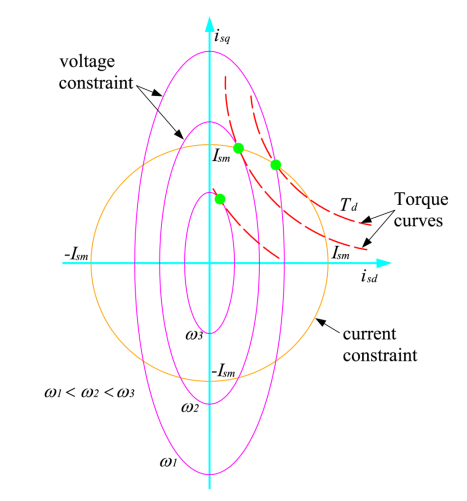
\includegraphics[width=7.5cm]{limit}}
				\caption{Feszültség limit ábrázolása különböző szögsebességeken}		
		 	\end{figure}
		 	
	\subsection{Szinkron sebesség meghatározása}	 
		
		A referencia áramokhoz tartozó állórész feszültségének számításához az egyenletekből adódóan szükséges a szinkron sebesség meghatározása. A szinkron sebesség értelmezhető a rotorban folyó áram, valamint a slip összegeként, és az állórész mágneses mezőjének forgási sebességét határozza meg. Akasztófa modellt alkalmazva a számolt mágnesező áram (${i}_{m}$) és főmező induktivitás szorzata eredményezi főmező fluxust ($\Psi_{M} $), mely ismeretében a slip sebesség meghatározható. A forgórész áramának szögsebessége a motor póluspárjainak és a mechanika szögsebesség szorzata, melyet a terhelőgép biztosít.
		
		\begin{align}
			& \omega_{slip} = \bigg| \frac{i_{qr} \cdot R_{r}}{\Psi_{M}} \bigg| \\
			& \omega_s = \omega_{slip} + ( \omega_m \cdot p )
		\end{align}
			
		\begin{figure}[!htb]
			\centering
			\label{mtpa_diag}
			\tcbox{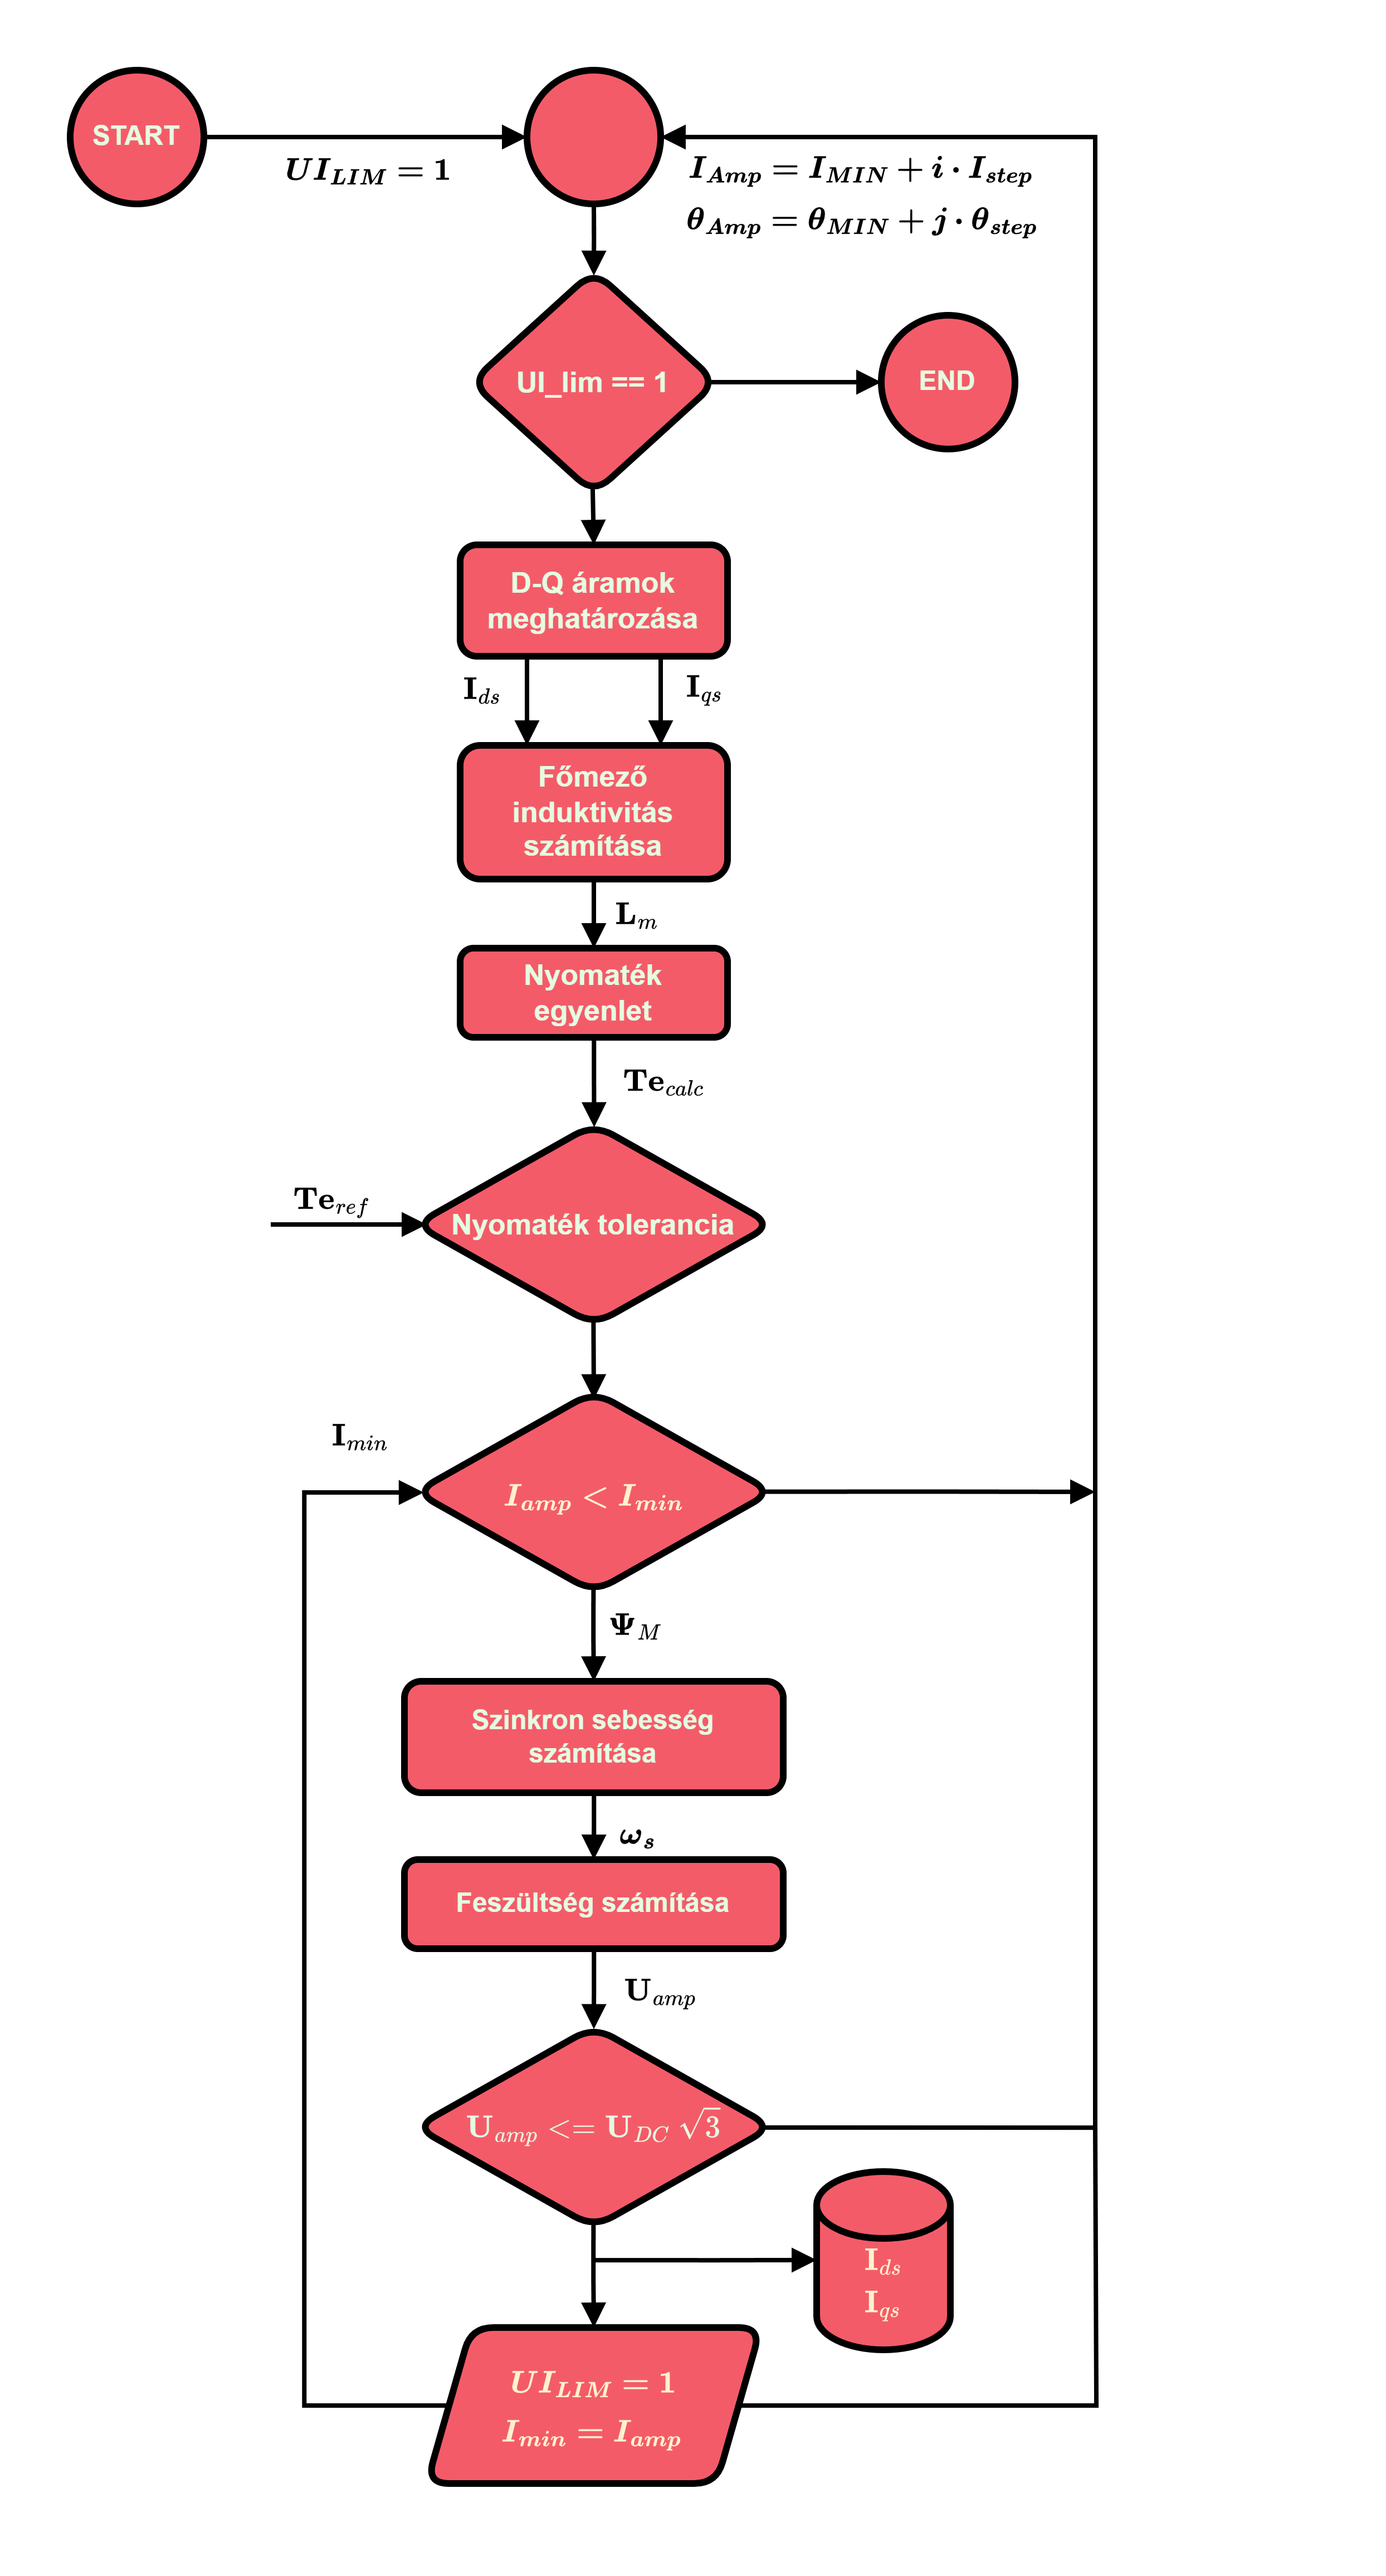
\includegraphics[width=11cm]{mtpa_diag}}
			\caption{MTPA folyamatábra }		
		\end{figure}
		\pagebreak
		
	\subsection{MTPA szimulációs eredmények}
			
		 
		 A MTPA stratégiát statikus és dinamikus főmező induktivitással is teszteltem, ugyanis a Simscapes motorblokk lehetővé teszi a mágneses telítődés ki-be kapcsolását. A terhelőgép sebessége 1000 RPM-re van beállítva. A nyomatékgörbék 10 Nm-től indulnak, és egészen addig rajzolódnak ki, ameddig beleférünk a kiadható maximális feszültségbe és áram limitbe. Két egymást követő nyomatékgörbe között 10 Nm eltérés van. A nyomatékgörbéket összekötött egyenesek pontjai tekinthetők az MTPA-nak. Az ábrát megfigyelve jól látható, hogy, a felhasznált motor paraméterek és invertervezérlésünk alapján a  maximális nyomaték értéke 100 Nm 1000 RPM-es terhelési sebesség mellet. Interpoláció alkalmazásával számolt munkapontok között is jó közelítéssel meg tudjuk találni a bementi paraméterekhez tartozó optimális áramokat. A gyorsabb keresést Look-Up table használatával tudjuk optimalizálni. 
		 
		 \begin{figure}[!htb]
		 	\centering
		 	\label{fig:mtpa_blokk}
		 	\tcbox{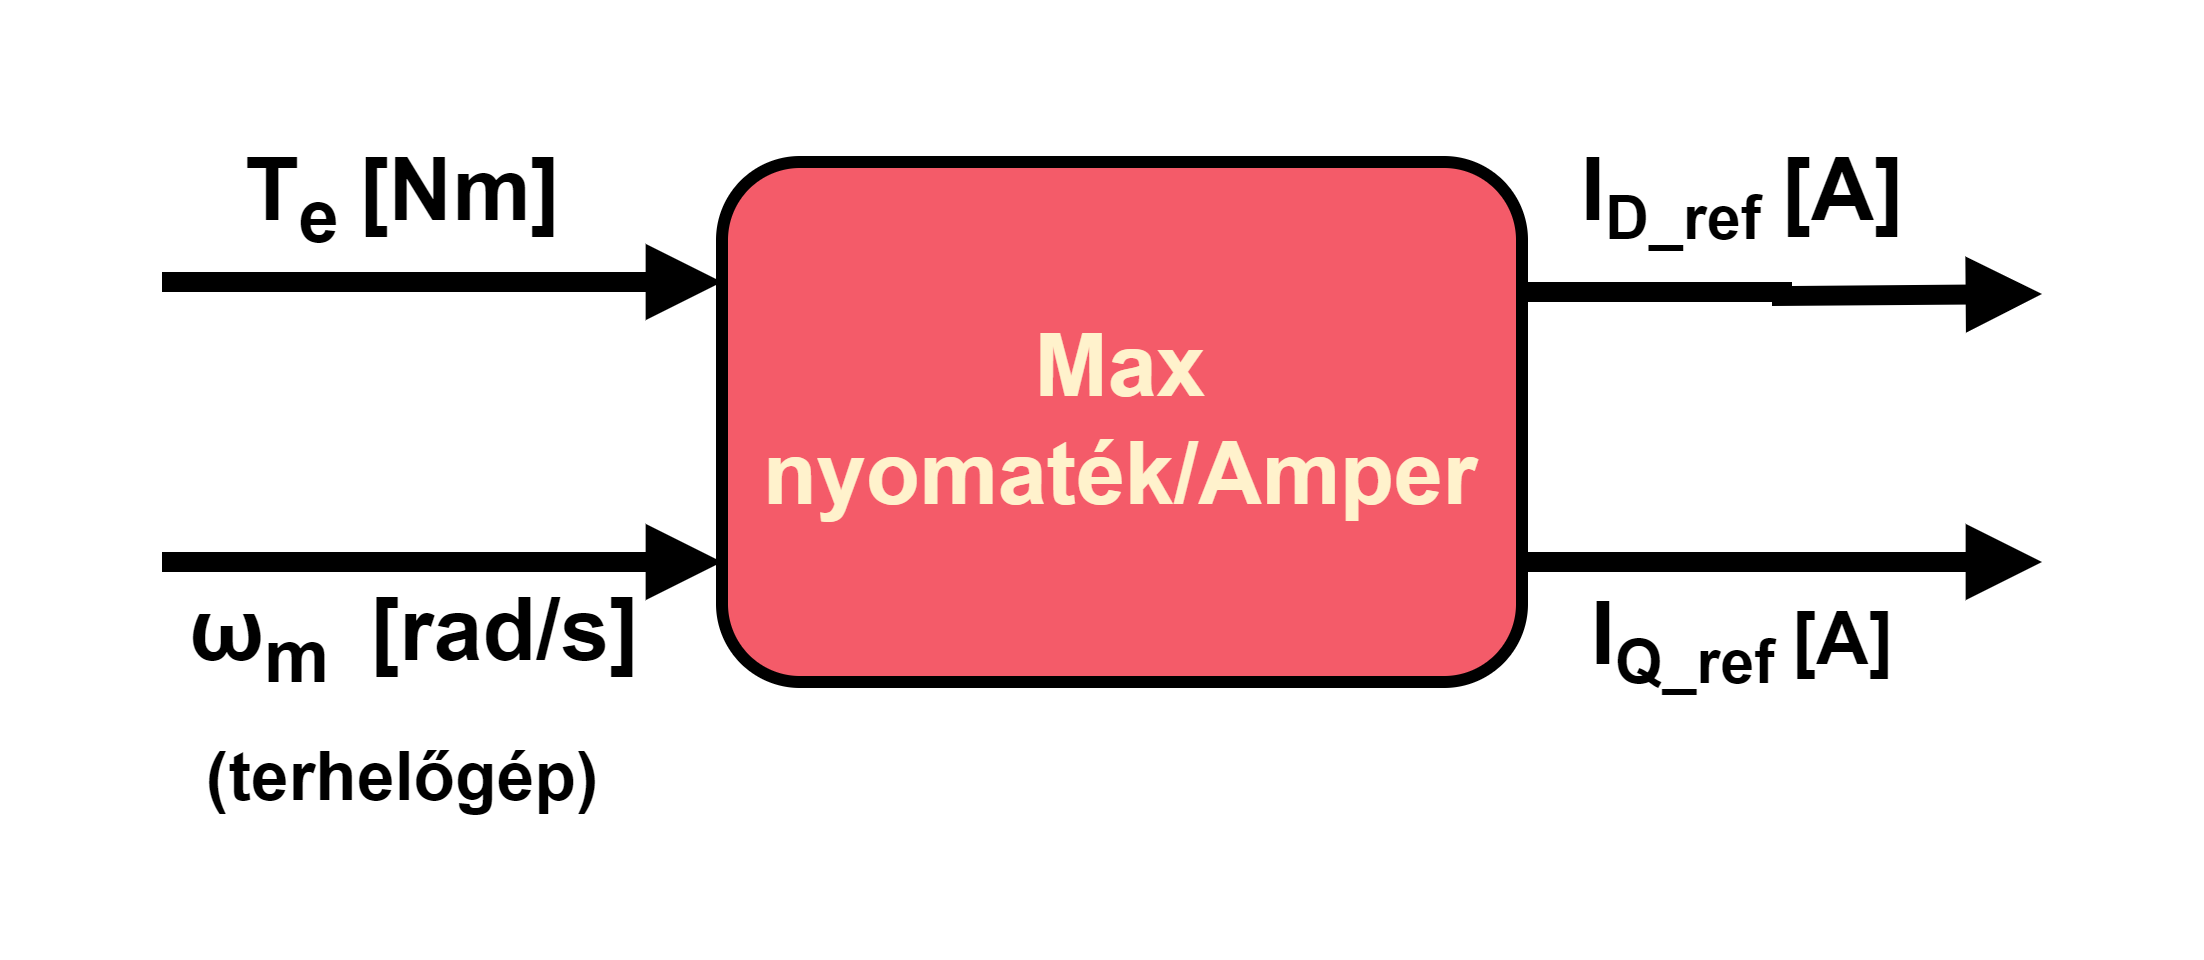
\includegraphics[width=6.5cm]{mtpa_blokk}}
		 	\caption{MTPA interfészei}		
		 \end{figure}
		 
		  \begin{figure}[!htb]
		 	\centering
		 	\label{fig:MTPA static}
		 	\tcbox{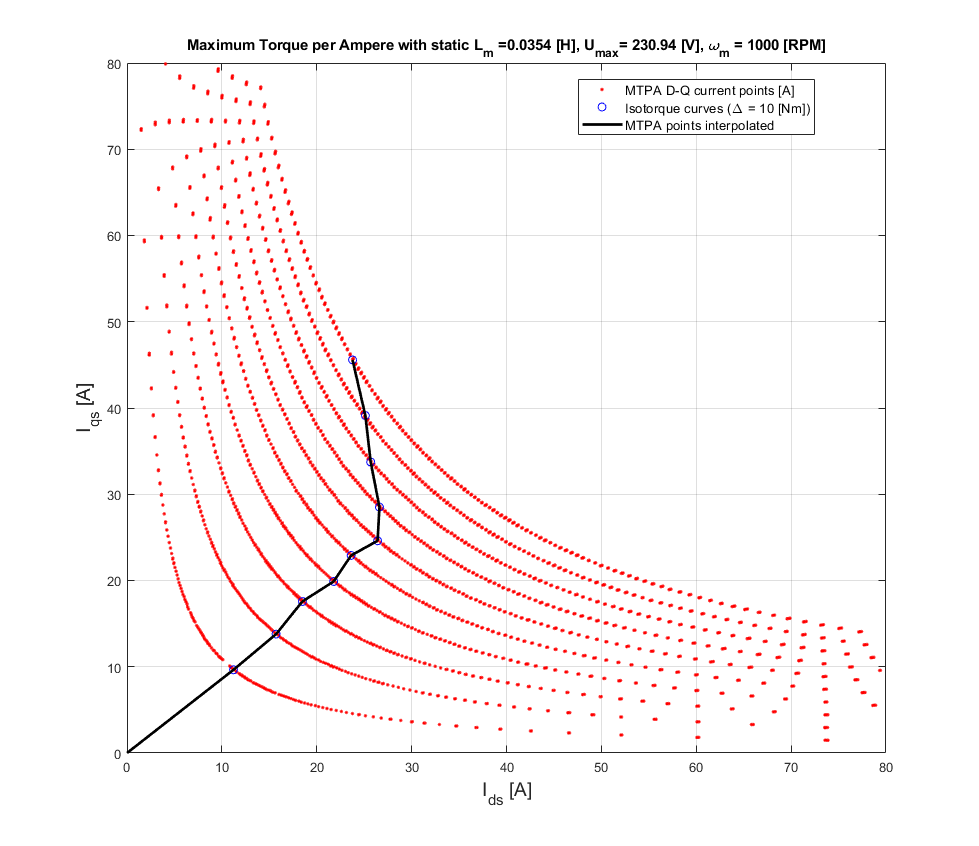
\includegraphics[width=10.5cm]{mtpa_static}}
		 	\caption{MTPA statikus $L_m$-el}		
		 \end{figure}
		 
		  \begin{figure}[!htb]
		 	\centering
		 	\label{fig:MTPA sat}
		 	\tcbox{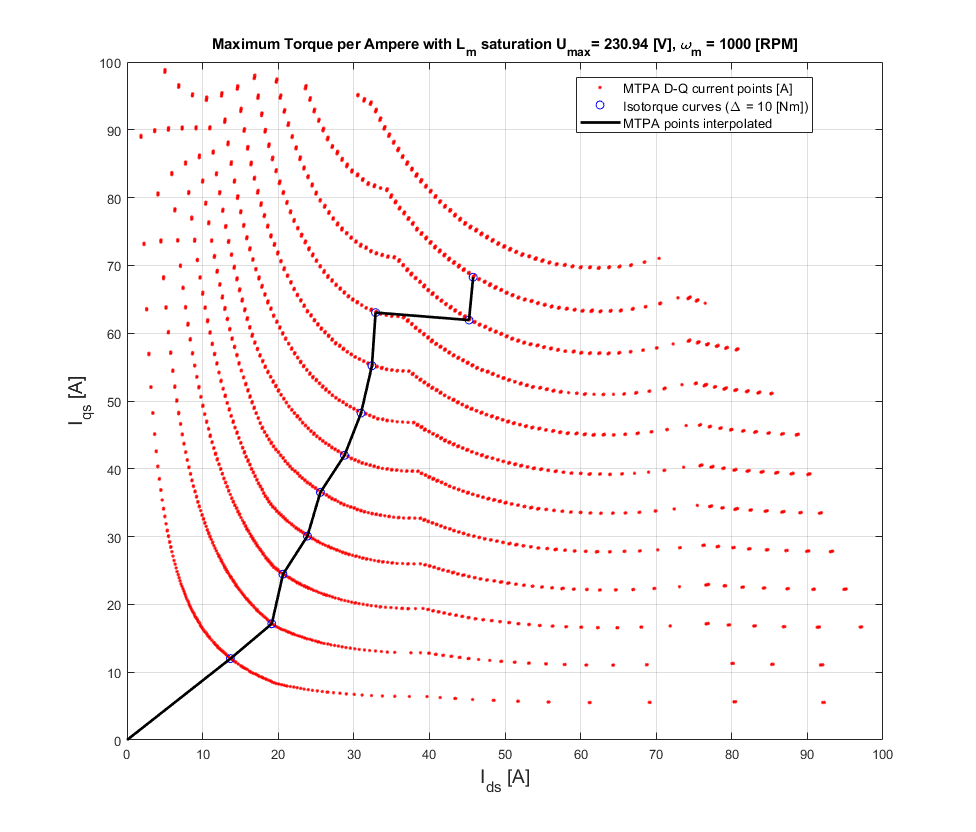
\includegraphics[width=10.5cm]{mtpa_sat}}
		 	\caption{MTPA mágneses telítődéssel}		
		 \end{figure}
		 
	\pagebreak
		 
	\section{D-Q áramszabályzók tervezése}	
		
		A nyomatékszabályozást áramszabályzással lehet megvalósítani. A kontroll modellben a hibajelet az MTPA által számolt referencia D-Q áramok és a motoron mért D-Q áramok különbsége fogja megadni. Az áramszabályzók kimenetei dimenzióban feszültségeknek tekinthetők, ugyanis ezek fogják meghatározni az invertervezérlést megvalósító térvektor moduláció bemeneteit. A megvalósítás során két áramszabályzót kell tervezni egyet a D-áramhoz, és egyet a Q-áramhoz, melyek felépítésükben diszkrét idejű PI szabályzók anti-windup technikával. Az áramszabályzók nem teljesen függetlenek egymástól, a motoron előálló két áram egymásra gyakorolt hatását, az áramszabályzók keresztcsatolásával lehet kompenzálni.
		
		\subsection {PI szabályzó folytonos modellje}
			
			\begin{align}
%				& y_{int}(t) = K_{i} \cdot \int{e(t)} \; dt +  \; y_{int}(0) \\
				& y_{PI}(t)  = K_{p} \cdot e(t)  + K_{i} \cdot \int{e(t)} \; dt + \; y_{int}(0)
			\end{align}
			
			\begin{itemize}
				\item $K_{p} $ $\leftarrow$ Arányos tag
				\item $T_{i} $ $\leftarrow$ Integrálási idő
				\item $ K_{i}=\frac{K_{p}}{T_{i}} $ $\leftarrow$ Integráló tag
			\end{itemize}

		\subsection{Euler és trapéz módszer }
		
			A szabályzó folytonos képletben lévő integrálást a mikrokontroller miatt diszkrét időben kell megoldani. A Forward - Euler vagy trapéz módszert alkalmas a diszkrét idejű integrálás elvégzéséhez. A trapéz módszer képlete az alábbi formában adható meg.
			
			\begin{align}
				& A = \int_{a}^{b} f(x) \; dx \approx \; \frac{b-a}{2} \cdot (\; f(a) + f(b) \; )			
			\end{align}
		
			Az (a) ábra a trapéz módszer vizualizációját , a (b) ábra pedig a integrálás időbeli vizualizációját mutatja. A (b) ábrán jól látható hogy az integrálás eredménye a [$ k-1 $] és a [$ k $]-dik időpillanat közötti hibajel változásának, és az eddigi integrálásnak ($ y_{int}[k-1] $) összege.
			
			\begin{align}
				& y_{int}[k] = \frac{Ts}{2} \cdot (\; e[k-1] + e[k]  \; ) \cdot K_{i} \; + \; y_{int}[k-1] \\
				& y_{PI}[k] = K_{p} \cdot e[n] \; + \;  y_{int}[k] 
			\end{align}
			
%			\begin{itemize}
%				\item $ \frac{b-a}{2} = \frac{Ts}{2} $ : mintavételi idő fele
%				\item $  y_{int}[k-1]$ : k-1 mintavételig integrált eredmény
%			\end{itemize}
			
			Forward - Eulert alkalmazva hasonló megvalósításhoz jutunk, azonban gyorsabb számolást eredményez.
			\begin{align}
				& y_{int}[k] = K_{i} \cdot (Ts \cdot  e[k] ) + y_{int}[k-1]
			\end{align}
			
			\begin{figure}[!htb]
				\centering
				\label{}
				\tcbox{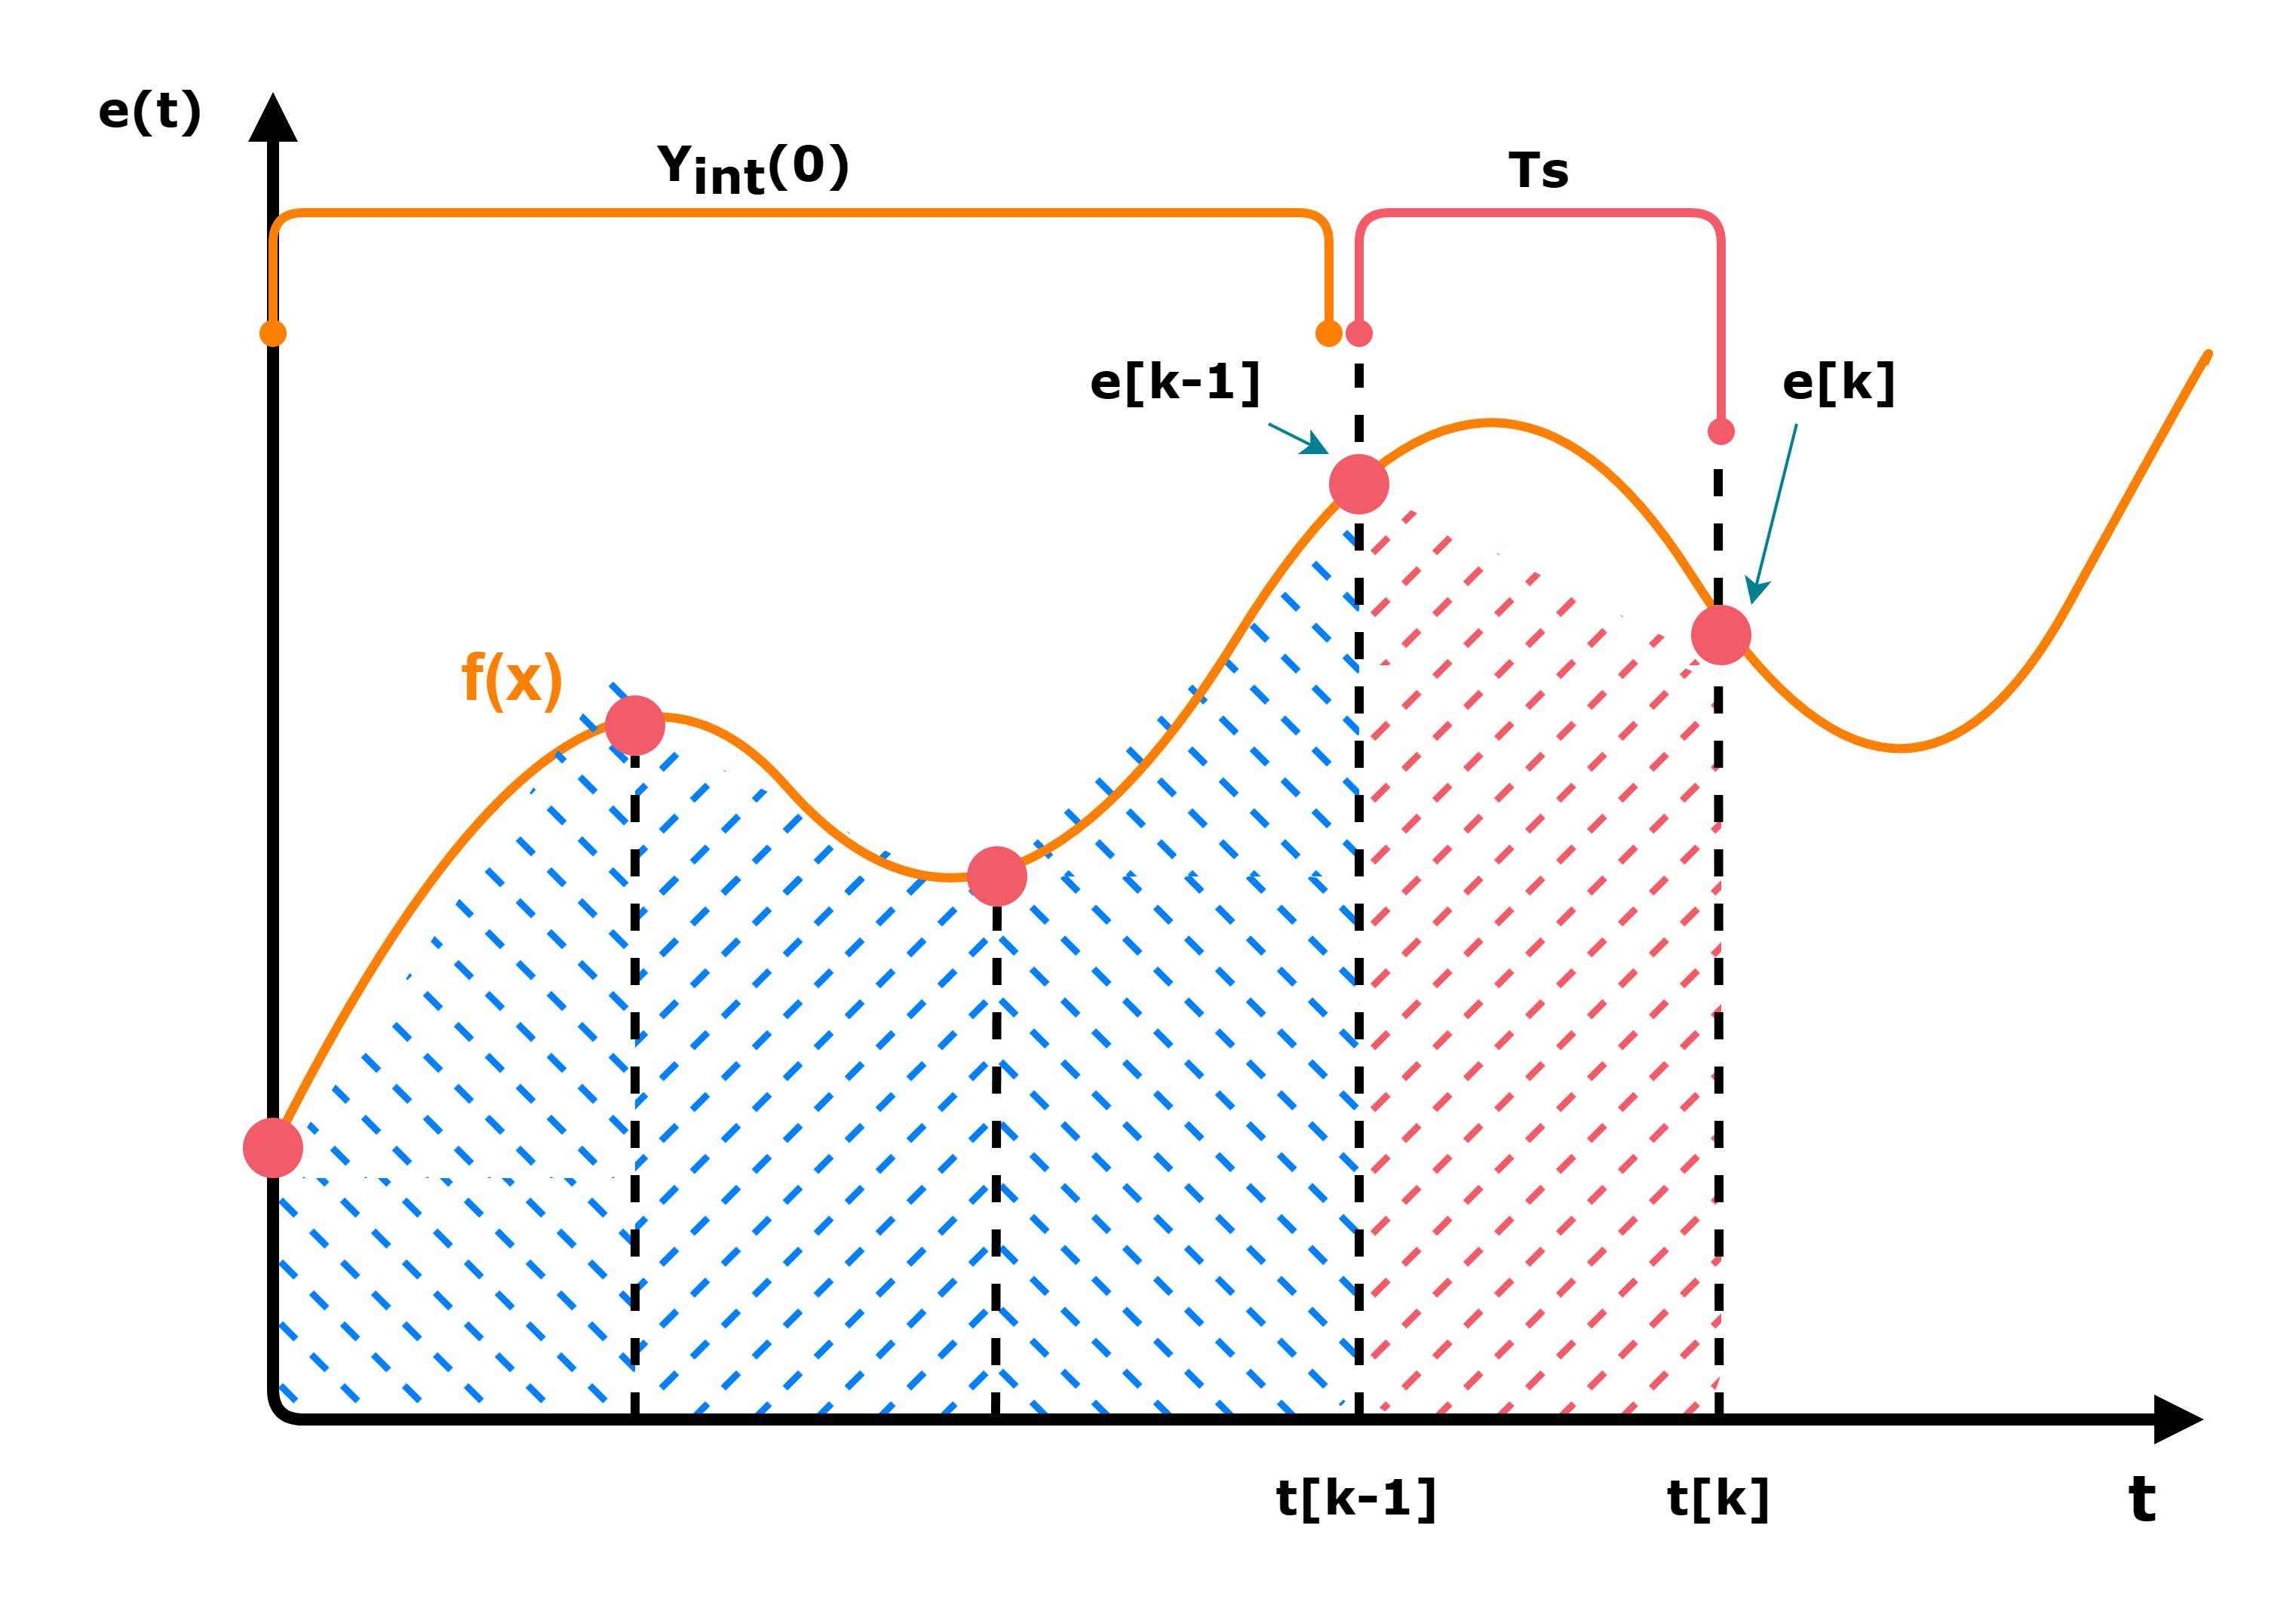
\includegraphics[width=11cm]{discretizedPi}}
				\caption{Diszkrét idejű integrálás ábrája}		
			\end{figure}
				 
		\pagebreak

		\subsection{Anti-windup technika }
		
			A szabályzók tervezése kapcsán figyelembe kell venni a térvektor modulációból kiadható maximális feszültséget. A szabályzóból kijövő beavatkozó jel maximuma ez az érték lesz, minimuma pedig ennek mínusz egyszerese, ugyanis az aktuátornak (inverter) ez a telítődési pontja. A beavatkozó jel korlátozása mellet az, integráló tagon is alkalmazni kell ezt a limitációt, bármelyik limit elérésekor az integrálást be kell fejezni. Limitáció nélkül az integráló tagból érkező jel a limiten túl is növekedne egészen addig, amíg a hibajel nem csökken. Ezt az integráló tag túlcsordulásának vagy "wind-up"-nak nevezzük.
			
			\begin{itemize}
				\item Ha az integráló tag bemenete eléri a maximum vagy minimum feszültség limitet, akkor nem integrálunk tovább, az integráló tag bemeneti érték lesz a kimenete is.
				\item Ha a szabályzó kimenete eléri a maximum vagy minimum feszültség limitet, akkor a szabályzó kimenete az ennek megfelelő feszültség limit lesz.
			\end{itemize}
			
			\begin{figure}[!htb]
				\centering
				\label{}
				\tcbox{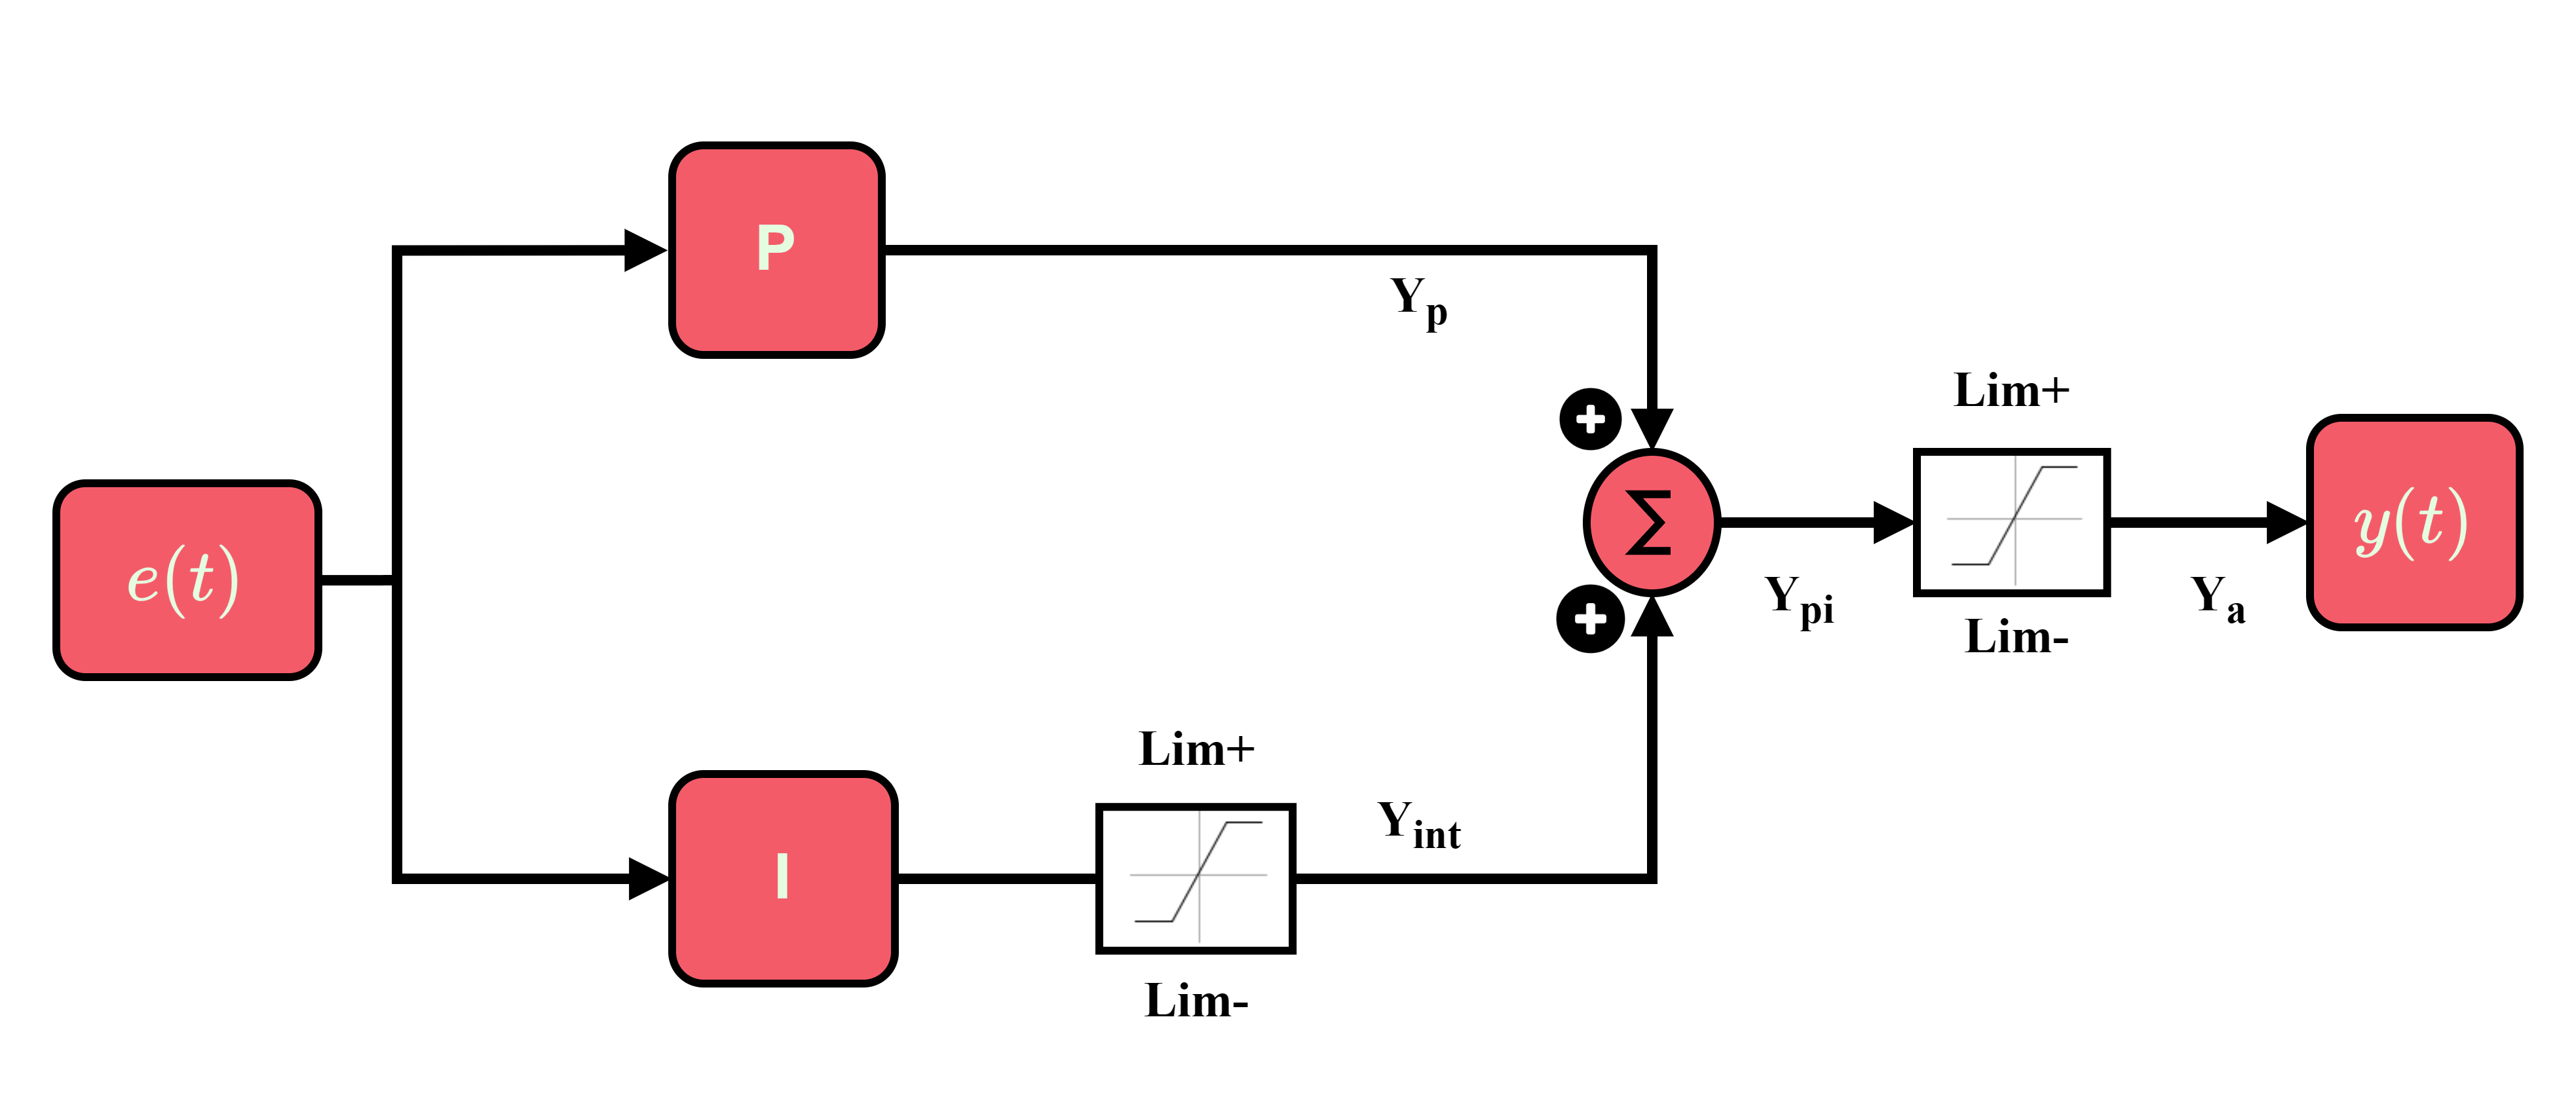
\includegraphics[width=8cm]{anti_Pi}}
				\caption{Diszkrét idejű PI szabályzó anti-windup technikával}		
			\end{figure}
			
			\begin{figure}[!htb]
				\centering
				\label{anti_windup}
				\tcbox{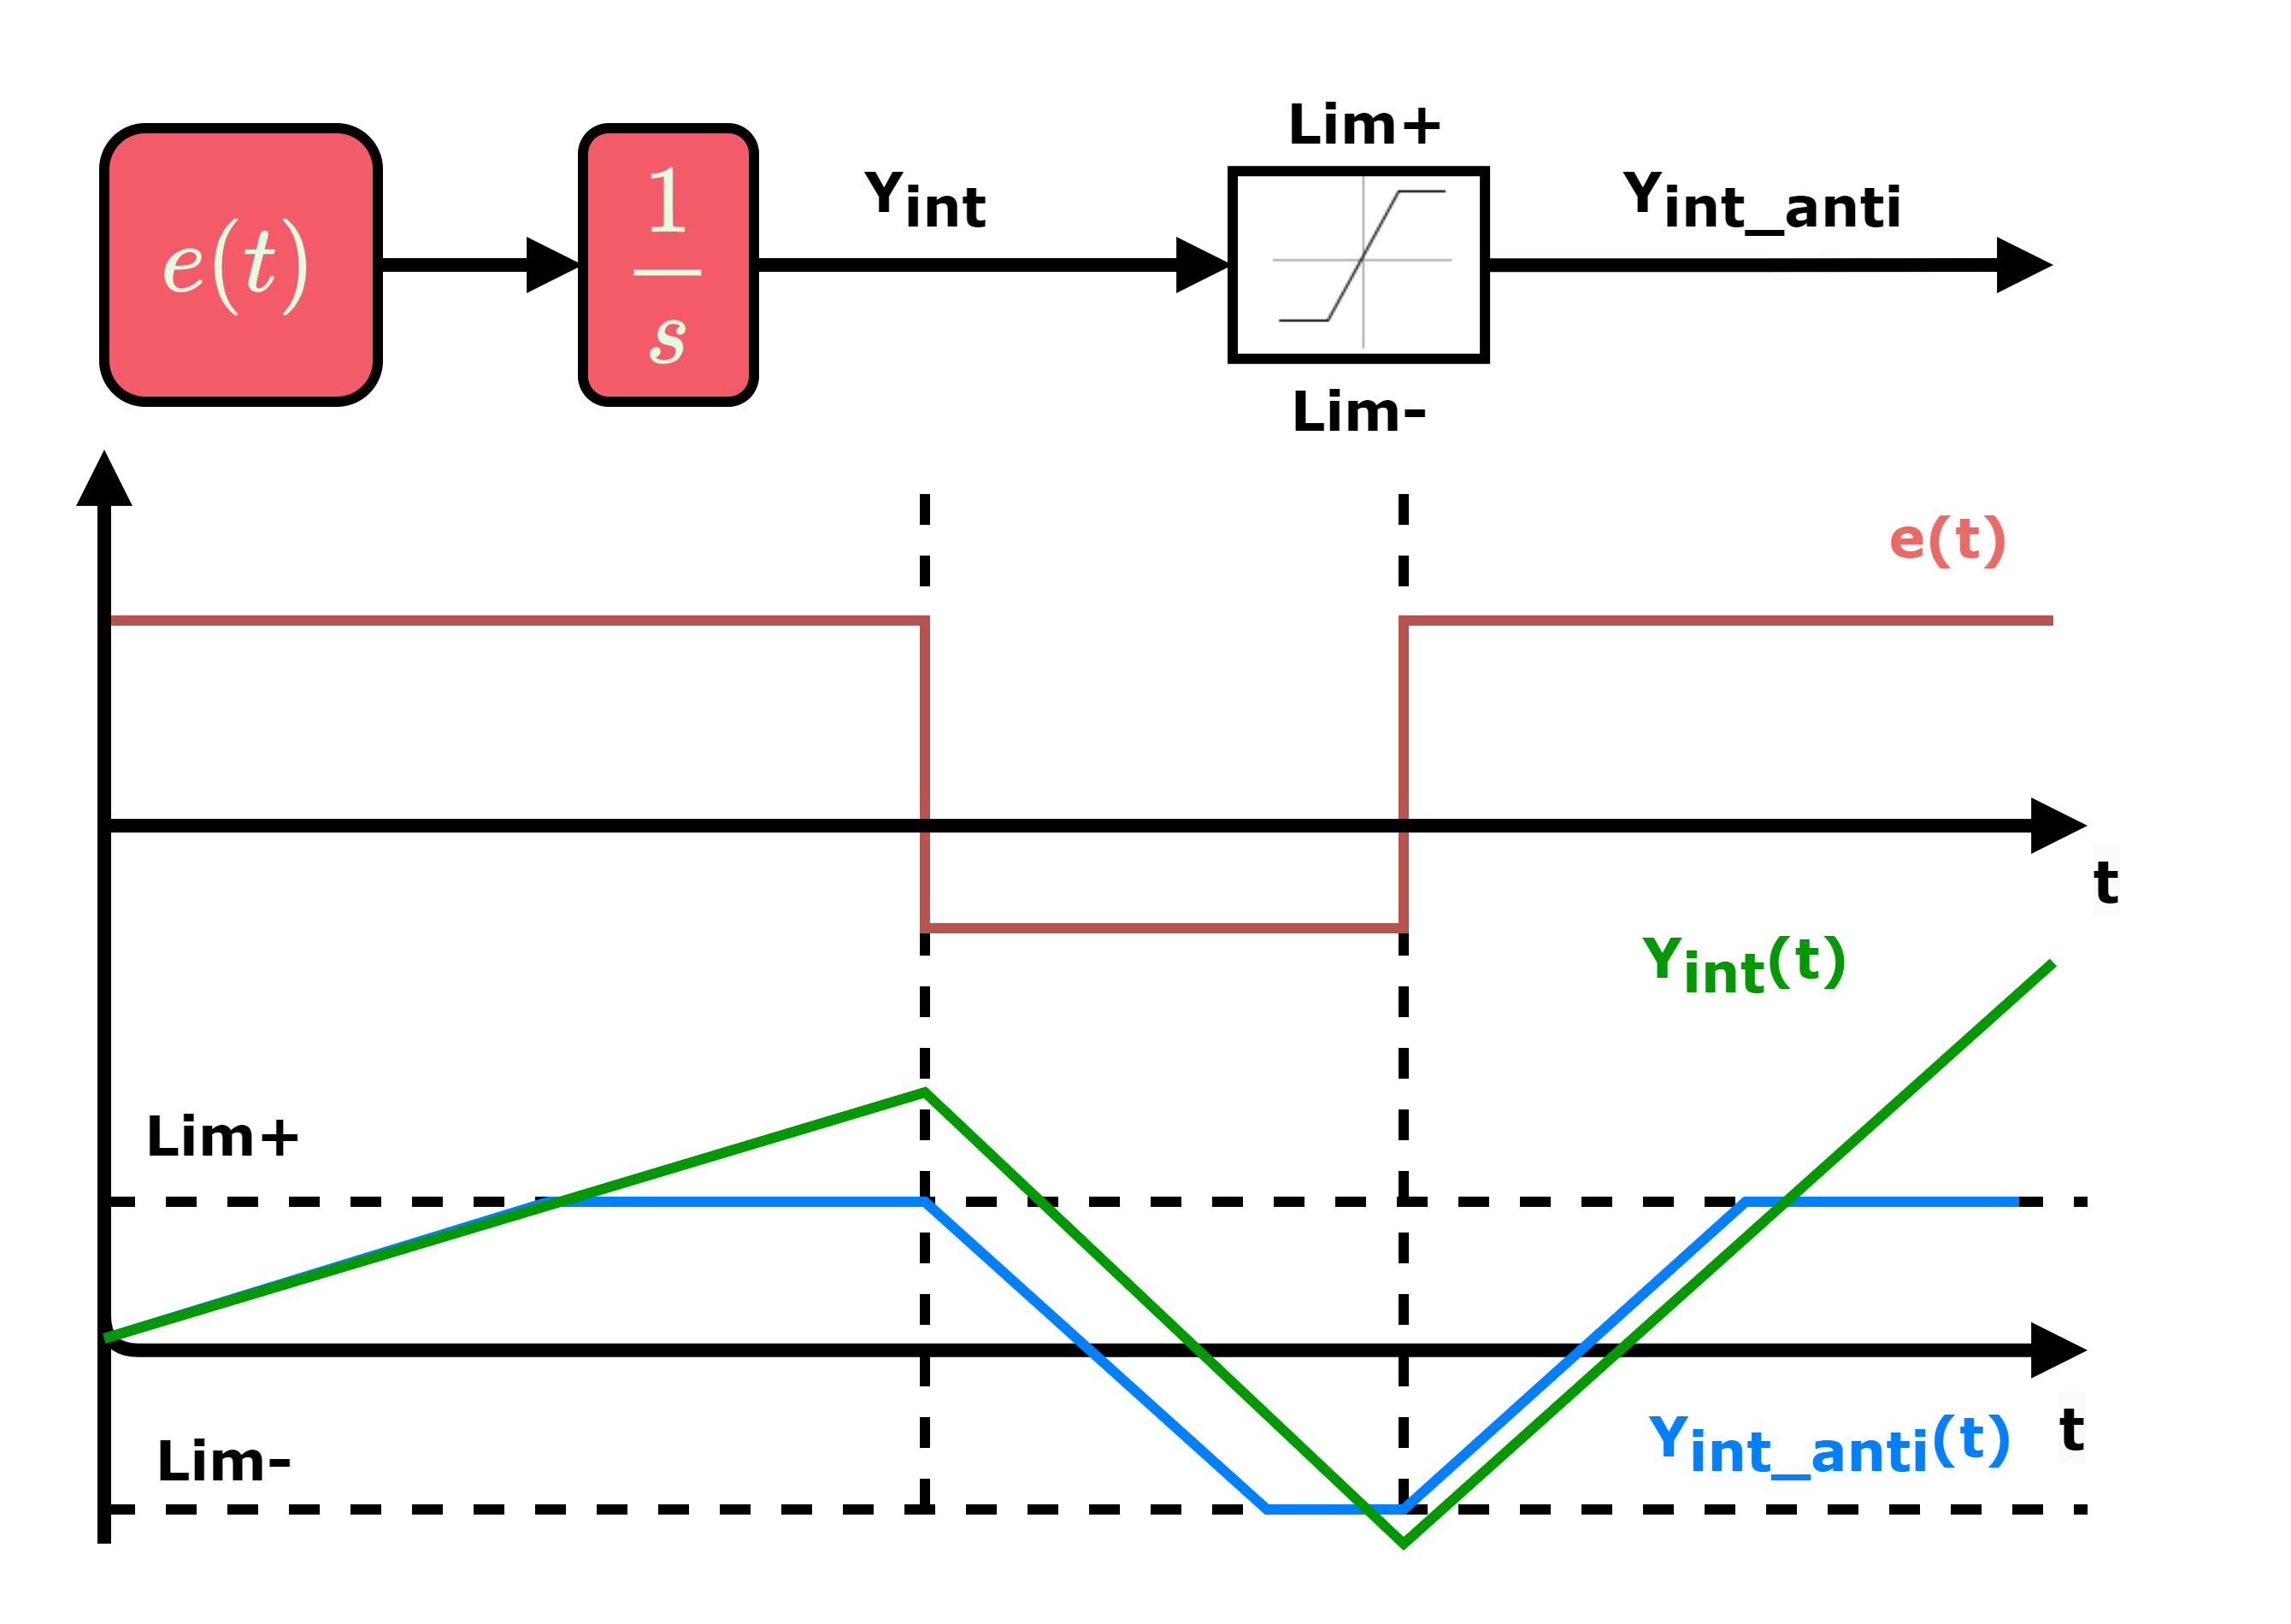
\includegraphics[width=10cm]{anti_windup}}
				\caption{ Integráló tag túlcsordulásának ábrázolása}		
			\end{figure}
			
			A (11) ábra a hibajel függvényében ábrázolja a szaturált integrátor és a korlátozás nélküli integráló tag kimenetét.
	
		\subsection{Áramszabályzó Simulinkes implementációja }
			
			A PI szabályzó diszkrét idejű megvalósítására számos implementáció létezik. Az anti-windup alkalmazása általános esetben két szaturációs blokkot igényel, az egyik az integráló tagot, a másik a kimenetet korlátozza. Szakdolgozatomban integrált PD szabályozót fogok használni mely működésben PI szabályzónak tekinthető. Előnye a hogy kimenet szaturációja megakadályozza integráló tag túlcsordulását is, így elég csak egy szaturációs blokk használata. Emellett a P tag bemenete a hibajel deriváltja. A szabályzó behangolása empirikus módon történt, a 2/3-ad szabály alkalmazásával Kezdetben $T_i$-t nagynak $A_p$-t kicsinek választjuk, és addig növeljük $A_p$ értékét, amíg túllendülést nem tapasztalunk. Ekkor $A_p$ értékét $\frac{2}{3}$-szorosára változtatjuk. A második lépésben $T_i$-t addig csökkentjük, amíg túllendülést tapasztalunk.
				
			\begin{itemize}
				\item Referencia jel :
				A referencia nyomatékhoz előállításához szükséges D - Q áramok, melyeket az MTPA számol. 
				\item Beavatkozó jel (kimenet) : 
				Dimenzióban feszültség, bemenete az Inverz Park transzformációnak.
				\item Visszacsatolt jel:
				A motoron mért áramok Park transzformáltjai.
			\end{itemize}
			

				\begin{equation}
					u[k]= (e[k-1] - e[k])\cdot K_{pd} + e[k] \cdot K_i + u[k-1]
					\label{eq: Implementált PI szabályzó egyenlete}					
				\end{equation}
		
			
			\begin{figure}[!htb]
				\centering
				\label{Pi_sim}
				\tcbox{\includegraphics[width=14cm]{Pi_sim}}
				\caption{Áramszabályzó implementációja}		
			\end{figure}
			
			\pagebreak	
		
	\section{Háromfázisú két szintű inverter bemutatása}
	
			\subsection{Az inverter általános felépítése}
		
				Az inverter egy olyan elektronikus átalakító, mely megfelelő irányítással egyenfeszültségből váltakozó feszültséget képes előállítani (DC $\rightarrow$ AC). Három fázis esetén a létrejövő váltófeszültségek fázisszöge 120 $^{\circ}$ - ban tér el egymástól. Két szint esetén a kiadható feszültségvektorok $ U_{DC} / 2  $ vagy $ -U_{DC} / 2 $ értéket vehetnek fel. Minden fázishoz egy hídág tartozik, melyen kettő darab, egy alsó ($ -U_{DC} / 2 $) és felső ( $ U_{DC} / 2 $ ) kapcsolóelem található. Ezek általában IGBT (izolált kapuzású bipoláris tranzisztorok) vagy FET-ek. Az iparban az IGBT-k használata elterjedtebb ugyanis, a veszteségek tekintetében optimálisabb, mint a FET-ek használata. A megfelelő egyenirányítás, valamint a kapcsolóelemek fizikai védelme miatt minden IGBT-hez tartozik egy ellenpárhuzamos dióda. A tranzisztorokat a GATE bemenettel tudjuk vezérelni, mely feszültségmentesen zárt állapotot eredményez, ami azt jelenti, hogy a tranzisztor nem vezet. Amikor a GATE bemenetre egy bizonyos küszöbfeszültség feletti feszültséget alkalmazunk, a tranzisztor vezető állapotba kerül, és áram folyik a Collector és az Emitter között. Ez a vezérlési módszer lehetővé teszi, hogy pontosan tudjuk szabályozni a fázisokon létrejövő feszültséget. A hídágak stabil feszültségszintjeinek biztosítása érdekében a feszültségforrással párhuzamos kondenzátor alkalmazása stabilabb működést eredményez, azonban ez főként többszintű inverterek irányításában kulcsfontosságú, ahol a DC feszültséget több részre kell osztani, emellett csökkenti a magas kapcsolási frekvenciából keletkező áramhullámosságot. A rövidzár elkerülése érdekében egy hídágban egyszerre csak egy IGBT lehet bekapcsolt (vezető) állapotban. Két szint esetén $2^3 = 8$ kapcsolási állapotot tudunk megkülönböztetni.
				
				
				\begin{figure}[!htb]
					\centering
					\label{inverter}
					\tcbox{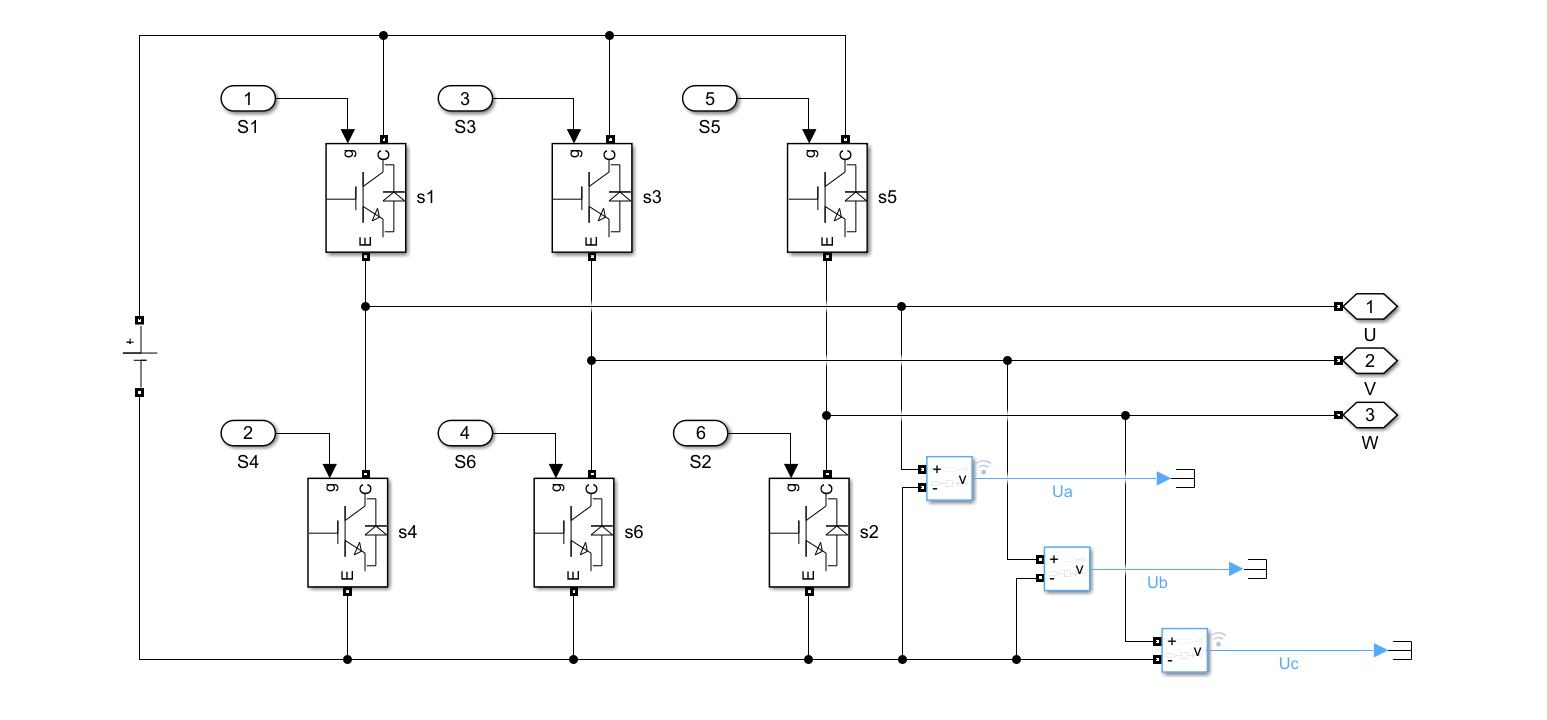
\includegraphics[width=15cm]{inverter}}
					\caption{ Kétszintű inverter áramköre}		
				\end{figure}
			\pagebreak		
			\subsection{Kapcsolási állapotok}
				 
				 	A különböző kapcsolási állapotok, eltérő feszültségeket eredményeznek a fázisok kimenetein, melyek egy csillagpontban vannak összekötve. Ha feltételezzük, hogy ellenállásuk egységes, a fázisokon eső feszültség meghatározható, minden kapcsolási állapothoz. Háromfázisú rendszereknél a kapcsolásokhoz tartozó fázis feszültségeket a komplex számsíkon is reprezentálhatjuk, melynek eredményeképpen térvektorokat (26) kapunk. Ezek nagysága egységesen $\frac{2}{3} \cdot U_{DC}$, szöghelyzetükben $ pi/3 $-rad-ban térnek el egymástól. Ezen térvektorok közül $U_7$ és $U_0$ nullvektornak, a többi aktív vektornak tekinthető. A térvektorokat ábrázolva egy hexagont tesznek ki.
				 		 
				\begin{align}
					& \vec{U}_{svec}= \frac{2}{3} \cdot ( U_{an} + a \cdot U_{bn} + a^{2} \cdot U_{cn} ) \\
					& a = e^{j \frac{2 \pi}{3}}  = cos \Pbracket{ \frac{2 \pi}{3} } + j \cdot sin \Pbracket{ \frac{2 \pi}{3} } = -\frac{1}{2} + \frac{\sqrt{3}}{2} j \\
					& a^{2} = e^{j \cdot \frac{4 \pi}{3}} = cos \Pbracket{ \frac{4 \pi}{3}} + j \cdot sin \Pbracket{ \frac{4 \pi}{3}} = -\frac{1}{2} - \frac{\sqrt{3}}{2} j \\
					& \vec{U}_{2} = \frac{2}{3} \cdot  \Pbracket{ \frac{1}{3} + \frac{1}{3} \cdot  \Pbracket{ - \frac{1}{2} + \frac{\sqrt{3}}{2} j}
					+  -\frac{2}{3} \cdot \Pbracket{ - \frac{1}{2} - \frac{\sqrt{3}}{2} j}} =  \frac{1}{3} + \frac{\sqrt{3}}{3} \cdot j\\
					& \varphi_{U_2} = \arctan{\frac{\Pbracket{ \frac{\sqrt{3}}{3} } } { \Pbracket{ \frac{1}{3} } }} = \frac{\pi}{3} = 60^{\circ}
				\end{align}
				
				\begin{figure}[!htb]
					\centering
					\label{states}
					\tcbox{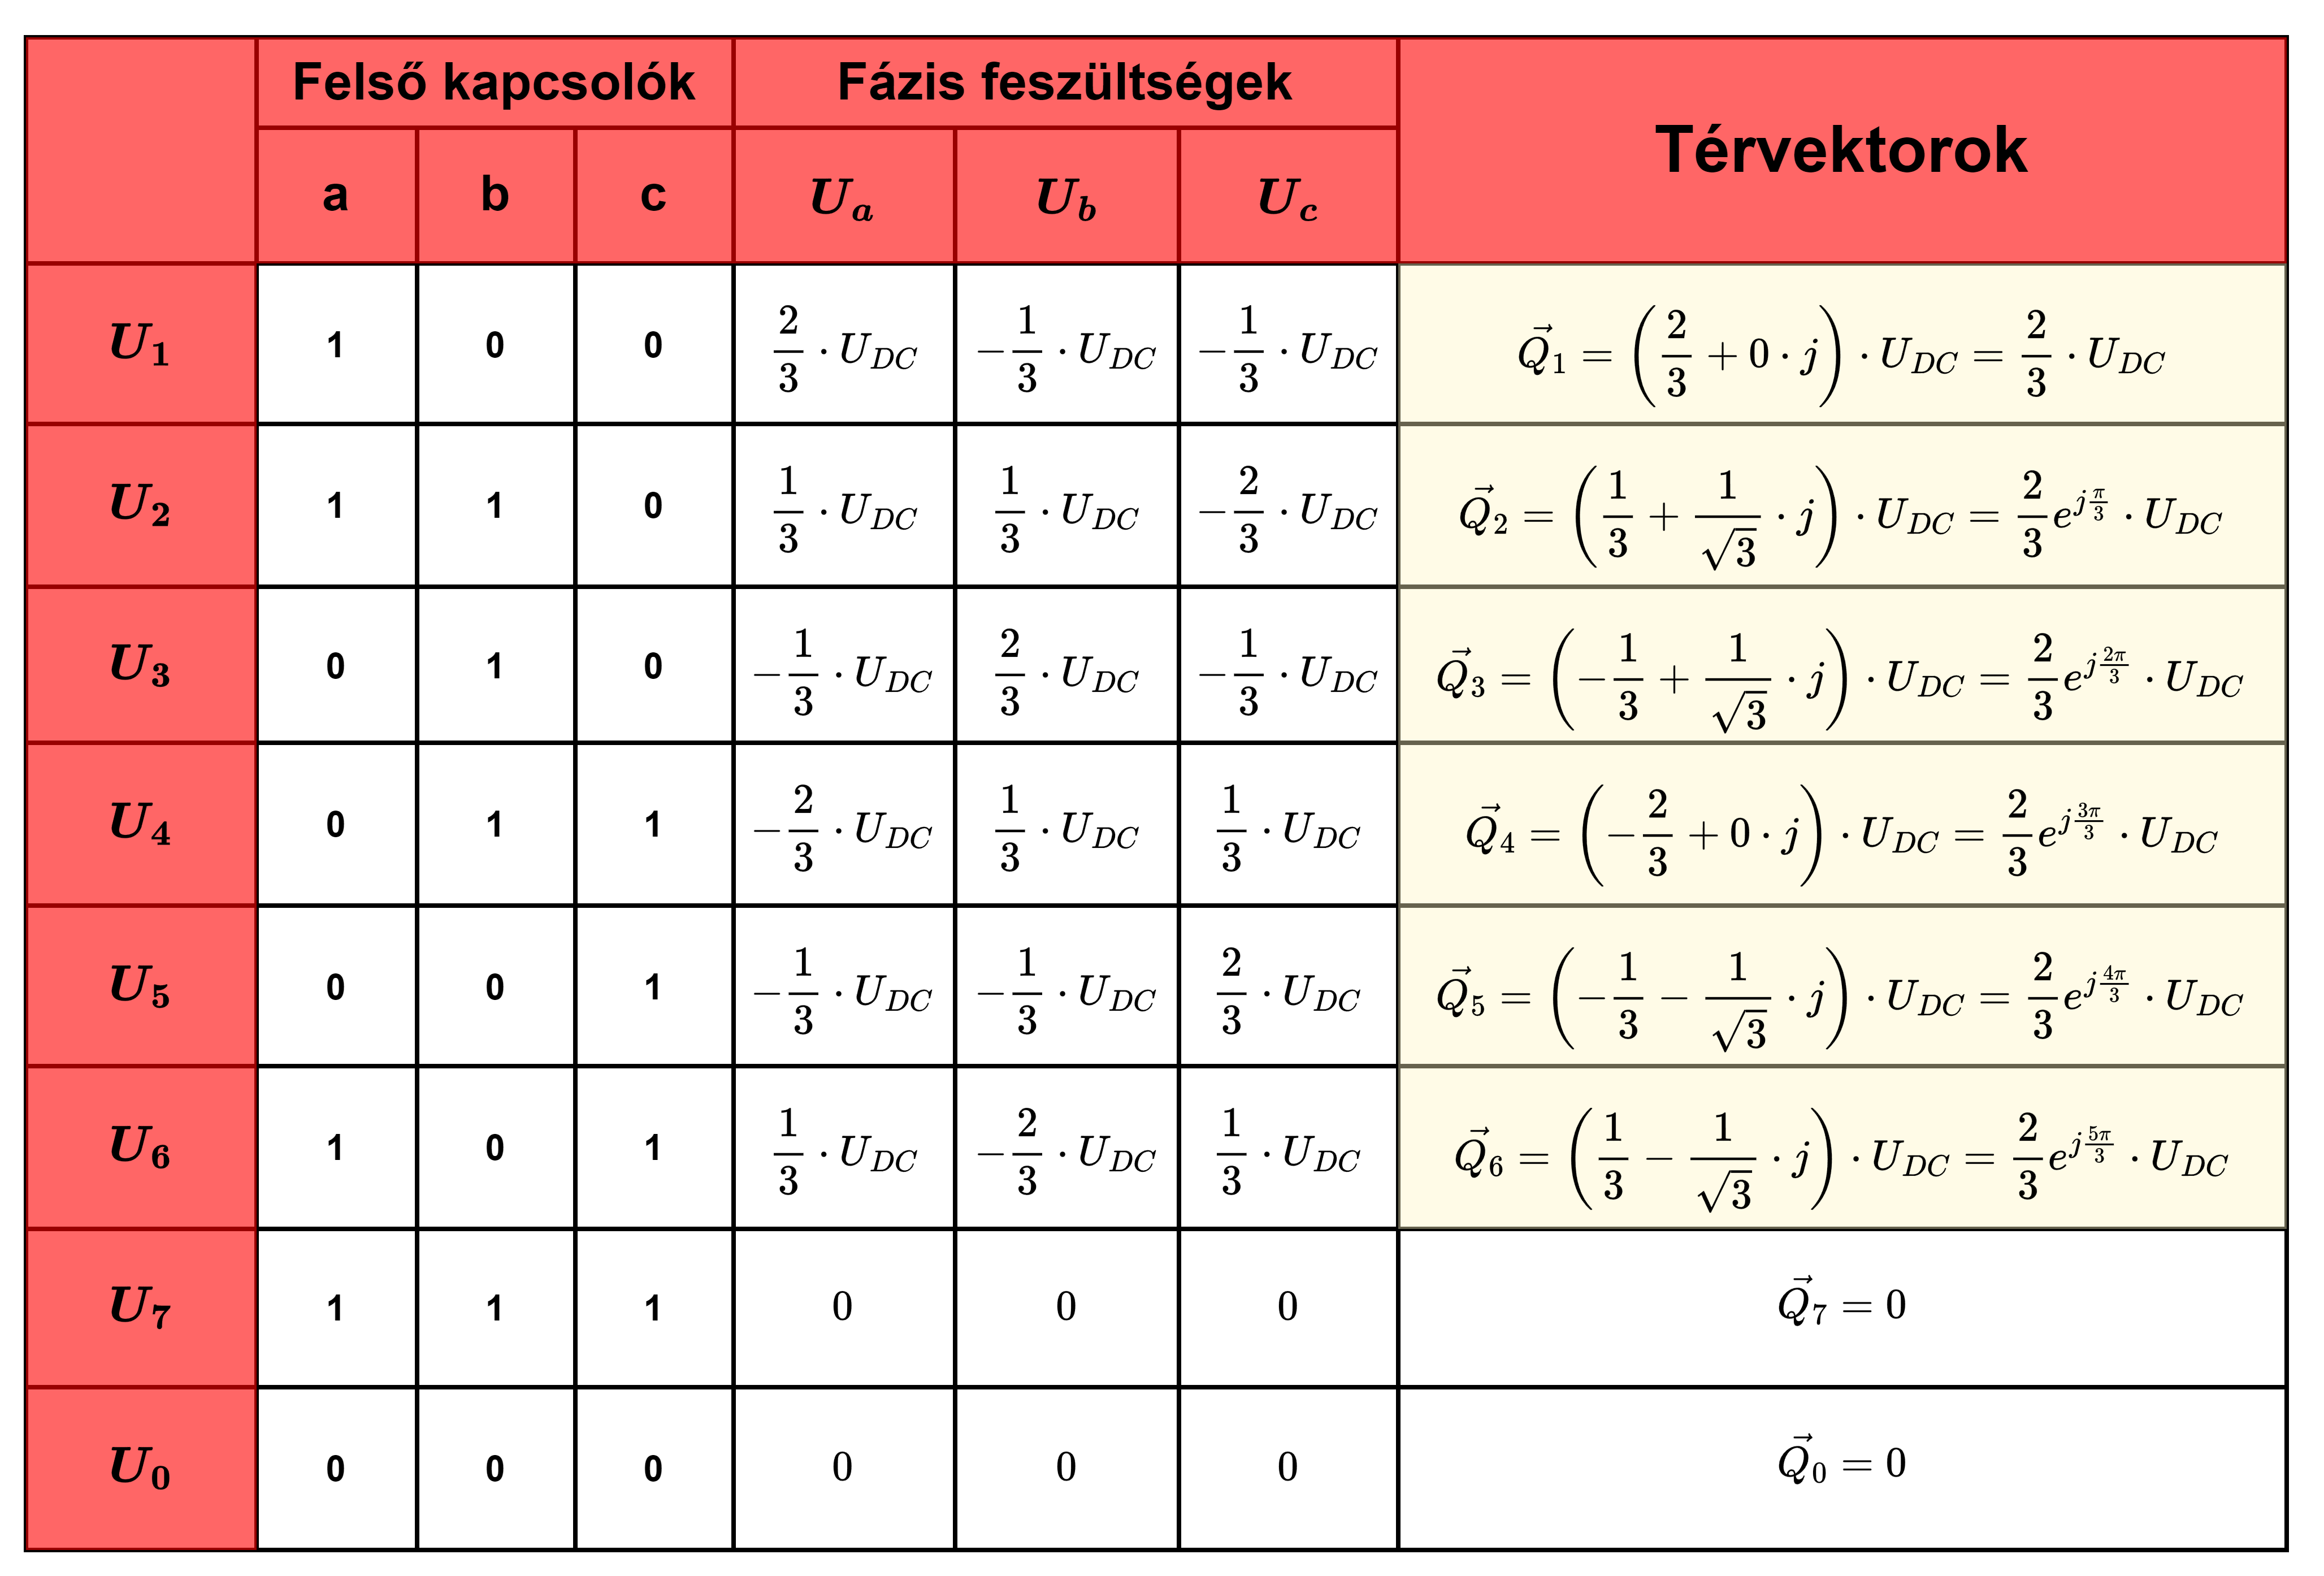
\includegraphics[width=11cm]{states}}
					\caption{ Kapcsolási állapotok térvektorai}		
				\end{figure}
					
			\section{Invertervezérlés tervezése  }
				\subsection{Térvektor (SVPWM) és szinuszos (SVM) moduláció összehasonlítása }
				
				A motoron létrejövő áramokat az inverter fázisfeszültségei határozzák meg. Az invertervezérlés célja, hogy az áramszabályzók által szolgáltatott beavatkozó jeleknek megfelelő fázisfeszültségeket generáljon. Ennek kivitelezése, a kapcsolók működéséhez szükséges PWM jel előállításával történik. Kétszintű inverter tekintetében a hatékonyságot a DC feszültség hatékony felhasználása, valamint az IGBT-k kapcsolási veszteségek minimalizálása határozza meg. Túlmodulálás nélkül szinuszos modulációval a fázisfeszültség maximális amplitúdója $ U_{DC} / 2 $ lehet, ilyenkor a modulációs index értéke $ m = 1 $. A modulációs index azt határozza meg, hogy a fázisfeszültségek amplitúdója $ U_{DC} / 2 $-hez képest hányszorosa lehet maximálisan túlmodulálás nélkül. Túlmodulálásnak azt a jelenséget nevezzük, amikor túllépjük a maximálisan felhasználható DC feszültséget. A DC feszültség hatékony felhasználásának mérőszáma a modulációs index. A térvektor moduláció során a szinuszos modulációhoz egy harmadik harmonikust keverünk hozzá, amely úgy módosítja a szinuszt, hogy a modulációs index maximális értéke $ 2 / \sqrt{3} = 1.15 $ is lehet. Tehát SPWM alkalmazásával a fázisfeszültségek maximális amplitúdója $ U_{DC}/\sqrt{3} $. Emellett az IGBT-ket is optimálisabban használja mint a szinuszos moduláció, ezzel csökkentve az áramhullámosságot és a kapcsolási veszteségeket.
				
				
					$$ U_{phase} = m \cdot \frac{U_{DC}}{2} \cdot \sin({\omega t + \phi}) $$
				
				\begin{figure}[!htb]
					\centering
					\label{sin_svpwm}
					\tcbox{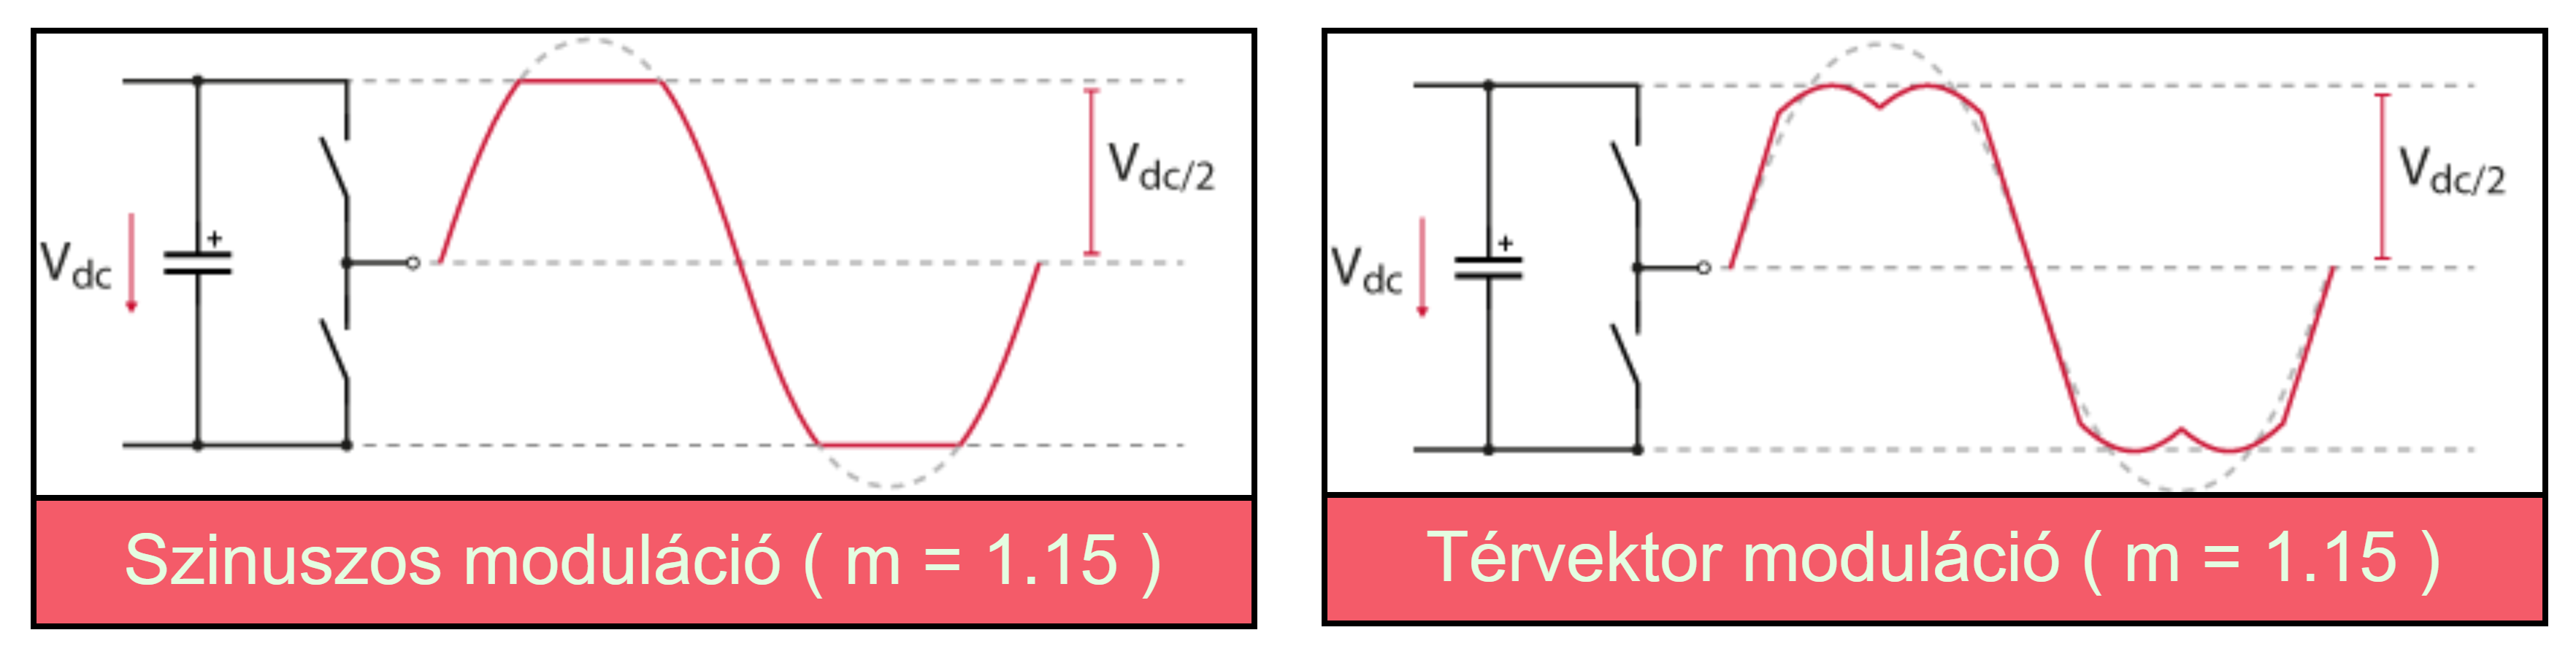
\includegraphics[width=15cm]{sin_svpwm}}
					\caption{SVM és SVPWM összehasonlítás}		
				\end{figure}
			
				\subsection{Térvektor moduláció bemutatása }
				
				A referencia feszültség térvektorának hossza és szöge Clarke-transzformáció alkalmazásával számítható. A transzformáció lényege, hogy egyszerűsíti háromfázisú rendszert és két fázisú álló (időfüggő) koordináta rendszerbe  képezi le. A tengelyek egymáshoz képest ortogonálisan helyezkednek el. A valós tengely elnevezése $ \alpha $, a képzetes $ \beta $.  A transzformáció bármilyen háromfázisú mennyiségre alkalmazható (feszültség, áram, fluxus). Az átalakítás során létrejön egy harmadik, zérus sorrendi összetevő, mely szimmetrikus rendszerek esetén nulla.
				
				\begin{figure}	
				\begin{equation*}
					\frac{2}{3} \cdot
					\renewcommand\arraystretch{1.5} % Adjust the vertical spacing
					\begin{bmatrix}
						1 & -\frac{1}{2} & -\frac{1}{2} \\
						0 & \frac{\sqrt{3}}{2} & -\frac{\sqrt{3}}{2}
					\end{bmatrix}
					\begin{bmatrix}
						U_a \\
						U_b \\
						U_c
					\end{bmatrix}
					=
					\begin{bmatrix}
						U_{\alpha} \\
						U_{\beta}
					\end{bmatrix}
				\end{equation*}
				\caption{Clarke transzformáció}
				\end{figure}
				\begin{align}
					& |\vec{U}_{ref}| = \sqrt{U_\alpha^2 + U_\beta^2} 
					& \Theta_{U_{ref}} = \arctan{\frac{U_\beta}{U_\alpha}}
				\end{align}
			
				A térvektorok által meghatározott hexagon hat egységes méretű szektorra osztható. A hexagonba beírható kör sugarának mérete $ U_{DC} /\sqrt{3} $. SVPWM során a térvektorokat kapcsolási idő alapján súlyozzuk. Egy szektorban kizárólag négy kapcsolási állapottal valósíthatjuk meg a referencia feszültséget. A négy kapcsolási állapot megfeleltethető az adott szektort határoló két aktív vektornak, valamint az $U_7$ és $U_0$ állapothoz tartozó nullvektoroknak. A nullvektorok minden szektorban elérhetőek. Ennek eredményeképpen három impulzusszélességet kapunk: $ T_{1} $, $ T_{2} $ a két aktív vektorhoz $ T_{0} $ pedig a nullvektorokhoz tartozik. Az impulzusszélességek összege megegyezik a mintavételi idővel ( $ T_s $).
				
				\begin{align}
					& T_{s} = T_{1} + T_{2} + T_{0}  \\
					& |U_{ref}| \cdot T_{s} = T_{1} \cdot |\vec{U}_{1}| + T_{2} \cdot |\vec{U}_{2}| + T_{0} \cdot |\vec{U}_{0}|
				\end{align}
				
				\begin{figure}[!htb]
					\centering
					\label{sTime1}
					\tcbox{\includegraphics[width=15cm]{sTime1}}
					\caption{ Szektor 1 szögeinek meghatározása}		
				\end{figure}
				
				\pagebreak
				Az 1-es szektorban a szögek kiszámolása után (14), szinusz - tétel alkalmazásával a  térvektorokhoz tartozó mindhárom impulzusszélesség meghatározható.
				\begin{align}
					& \frac{T_{1} \cdot |U_{1}|}{ \sin \Pbracket {\frac{\pi}{3} - \alpha }} 
					= \frac{T_{2} \cdot |U_{2}|}{ \sin \Pbracket {\alpha }} 
					= \frac{Ts \cdot |U_{ref}|} { \sin \Pbracket {\frac{2}{3} \pi }}
				\end{align}
				
				\begin{align}
					& \frac{T_{1} \cdot \frac{2}{3} \cdot U_{DC} }{ \sin \Pbracket {\frac{\pi}{3} - \alpha }}
				     = \frac{ Ts\cdot|U_{ref}|}{\frac{\sqrt{3}}{2}}
					& \frac{T_{2} \cdot \frac{2}{3} \cdot U_{DC} }{ \sin( \alpha )} 
					= \frac{ Ts\cdot |U_{ref}|}{\frac{\sqrt{3}}{2}} 
				\end{align}
				\begin{align}
					& T_{1} = Ts \cdot  \sqrt{3} \cdot \frac{|U_{ref}|}{U_{DC}}  \cdot \sin \Pbracket {\frac{\pi}{3} - \alpha }
					& T_{2} = Ts \cdot  \sqrt{3} \cdot \frac{|U_{ref}|}{U_{DC}}  \cdot \sin(\alpha )
				\end{align}
				
				
				
				 Modulációs index-el  $\Pbracket { m = \sqrt{3} \cdot \frac{|U_{ref}|}{U_{DC}}} $  egyszerűsítve az alábbi formát kapjuk: 
	
				\begin{align}
					& T_{1}  = Ts \cdot m \cdot \sin \Pbracket {\frac{\pi}{3} - \alpha }
					& T_{2} = Ts \cdot m \cdot \sin(\alpha ) &
					& T_{0} = Ts - (T_{1} + T_{2} )
				\end{align}
			
				A szektorok ($ n $) növelésével, csak az aktív térvektorok változnak, melyek $ +\frac{\pi}{3} $ változtatják térbeli elhelyezkedésüket. A szektor meghatározása a feszültség vektor szöghelyzetéből történik. Az impulzusszélességek általános formulája csak a szinuszos kifejezésben módosul szektor 1-hez képest. Ez alapján $ T_{1} $ esetében hozzáadunk, $ T_{2} $ - nél kivonunk $ \Pbracket { \frac{n-1}{3} \cdot \pi }$ - t a szinuszos kifejezésben.
				
				
				\begin{align}
					& T_{1}  = Ts \cdot m \cdot \sin \Pbracket {\frac{\pi}{3} - \alpha + \Pbracket { \frac{n-1}{3} \cdot \pi }  } \\
					& T_{1} = Ts \cdot m \cdot \sin \Pbracket {  \frac{n \cdot \pi}{3} - \alpha } 
					& T_{2} = Ts \cdot m \cdot \sin \Pbracket { \alpha -  \frac{(n-1) \cdot \pi }{3} } 
				\end{align}
				
				A kapcsolási veszteségek minimalizálása érdekében, az inverter egy kapcsolási periódusához tartozó periódusidő hét szegmensre van osztva, melyben a négy vektorhoz kiszámolt impulzusszélességeket további részekre osztjuk. Ennek előnye, hogy egy szegmensből, a következő szegmensbe történő váltás esetén, csak egy hídágon módosítjuk a kapcsolók állapotát, valamint egy mintavételi idő alatt minden kapcsolót egyszer kapcsolunk vezető és kikapcsolt állapotba. A kapcsolási szekvenciák alapján statikus kapcsolási táblákat tudunk létrehozni minden szektorhoz, amelyekben szektoronként csak az impulzusszélességek változnak, melyeknek teljesítik az alábbi szabályokat.
				
				\begin{enumerate}
					\item  Minden szegmens idejének egyenlőnek kell lenni $Ts$-el.
					\newline ($ T_{1} + T_{2} + T_{0} =  T_{s} $)
					
					\item Egy szegmensből , a következő szegmensbe történő váltás esetén az egy hidágon lévő két IGBT kapcsolási állapotát módosítjuk
					
					\item A mintavételi periódus közepén a kapcsolási állapot [111] van kiválasztva $\frac{T_{0}}{2}$  ideig, míg a 
					kapcsolási szekvencia 1. és 7. szegmensében, a [000] állapot kerül felhasználásra egyenként $\frac{T_{0}}{4}$  ideig.
					
					\item Egy mintavételi idő alatt minden kapcsolót egyszer kapcsolunk vezető és kikapcsolt állapotba.
					
					\item A kapcsolási frekvenciának ($F_{sw}$) egyenlőnek kell lennie a mintavételi frekvenciával ($F_{sp}$).
					\newline $F_{sw} =F_{sp} = \frac{1}{T_{s}}$  
				\end{enumerate}
				\hfill\break
				\hfill\break
				\begin{figure}[!htb]
					\centering
					\label{swSeq}
					\tcbox{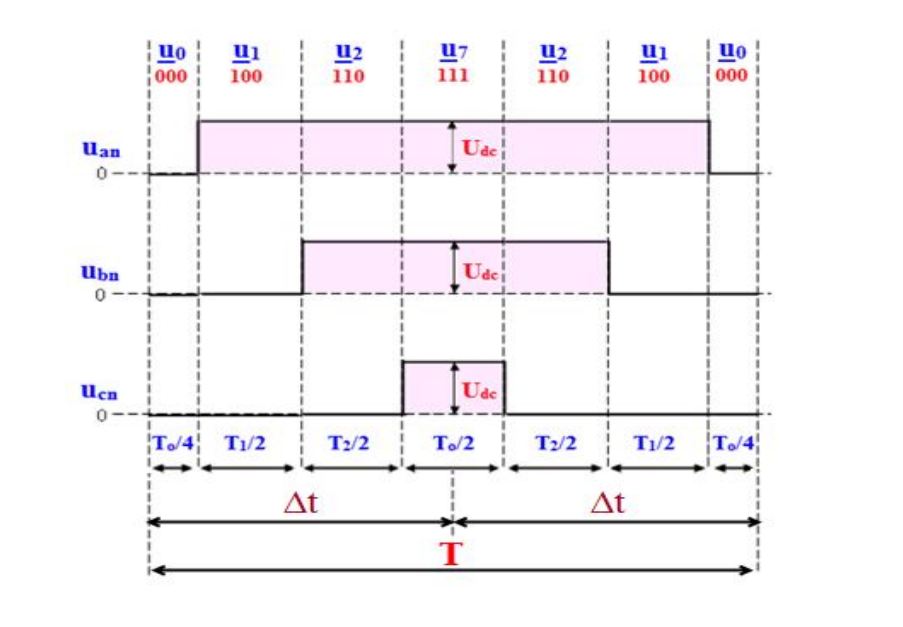
\includegraphics[width=14cm]{swSeq}}
					\caption{ Kapcsolási szekvencia sector 1-hez}		
				\end{figure}
				
				\begin{figure}[!htb]
					\centering
					\label{swTable}
					\tcbox{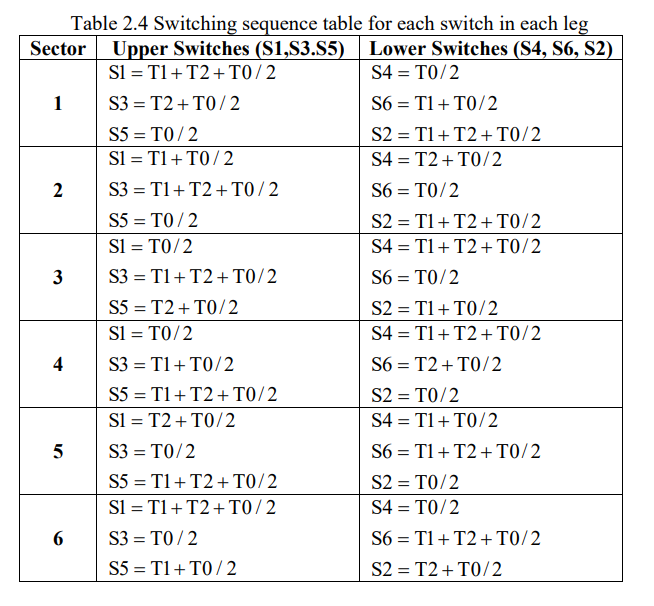
\includegraphics[width=9cm]{swTable}}
					\caption{Kapcsolási táblázat szektoronként}		
				\end{figure}
		
				\pagebreak
			
				A kapcsolók vezérlését PWM jelek végzik. Az eddigi lépések a kapcsolók kitöltési tényezőjét eredményezik, amely a moduláló jelnek tekinthető. Az inverter kapcsolási sebességét a vivőjel határozza meg, amely egy háromszög jel. Mindkét jel minimum és maximum értéke nulla  és egy. A vivőjel és a moduláló jel összekomparálásából megkapjuk a kapcsolókhoz tartózó PWM jeleket. Ha a moduláló jel nagyobb egyenlő, mint a vivőjel a PWM értéke 1 lesz, ellenkező esetben 0. Az egy hídágban lévő kapcsolók egymás negáltjai, így minden hídághoz elég csak az egyik kapcsoló PWM-jének kiszámolása.
				
				\begin{figure}[!htb]
					\centering
					\label{PWM gen}
					\tcbox{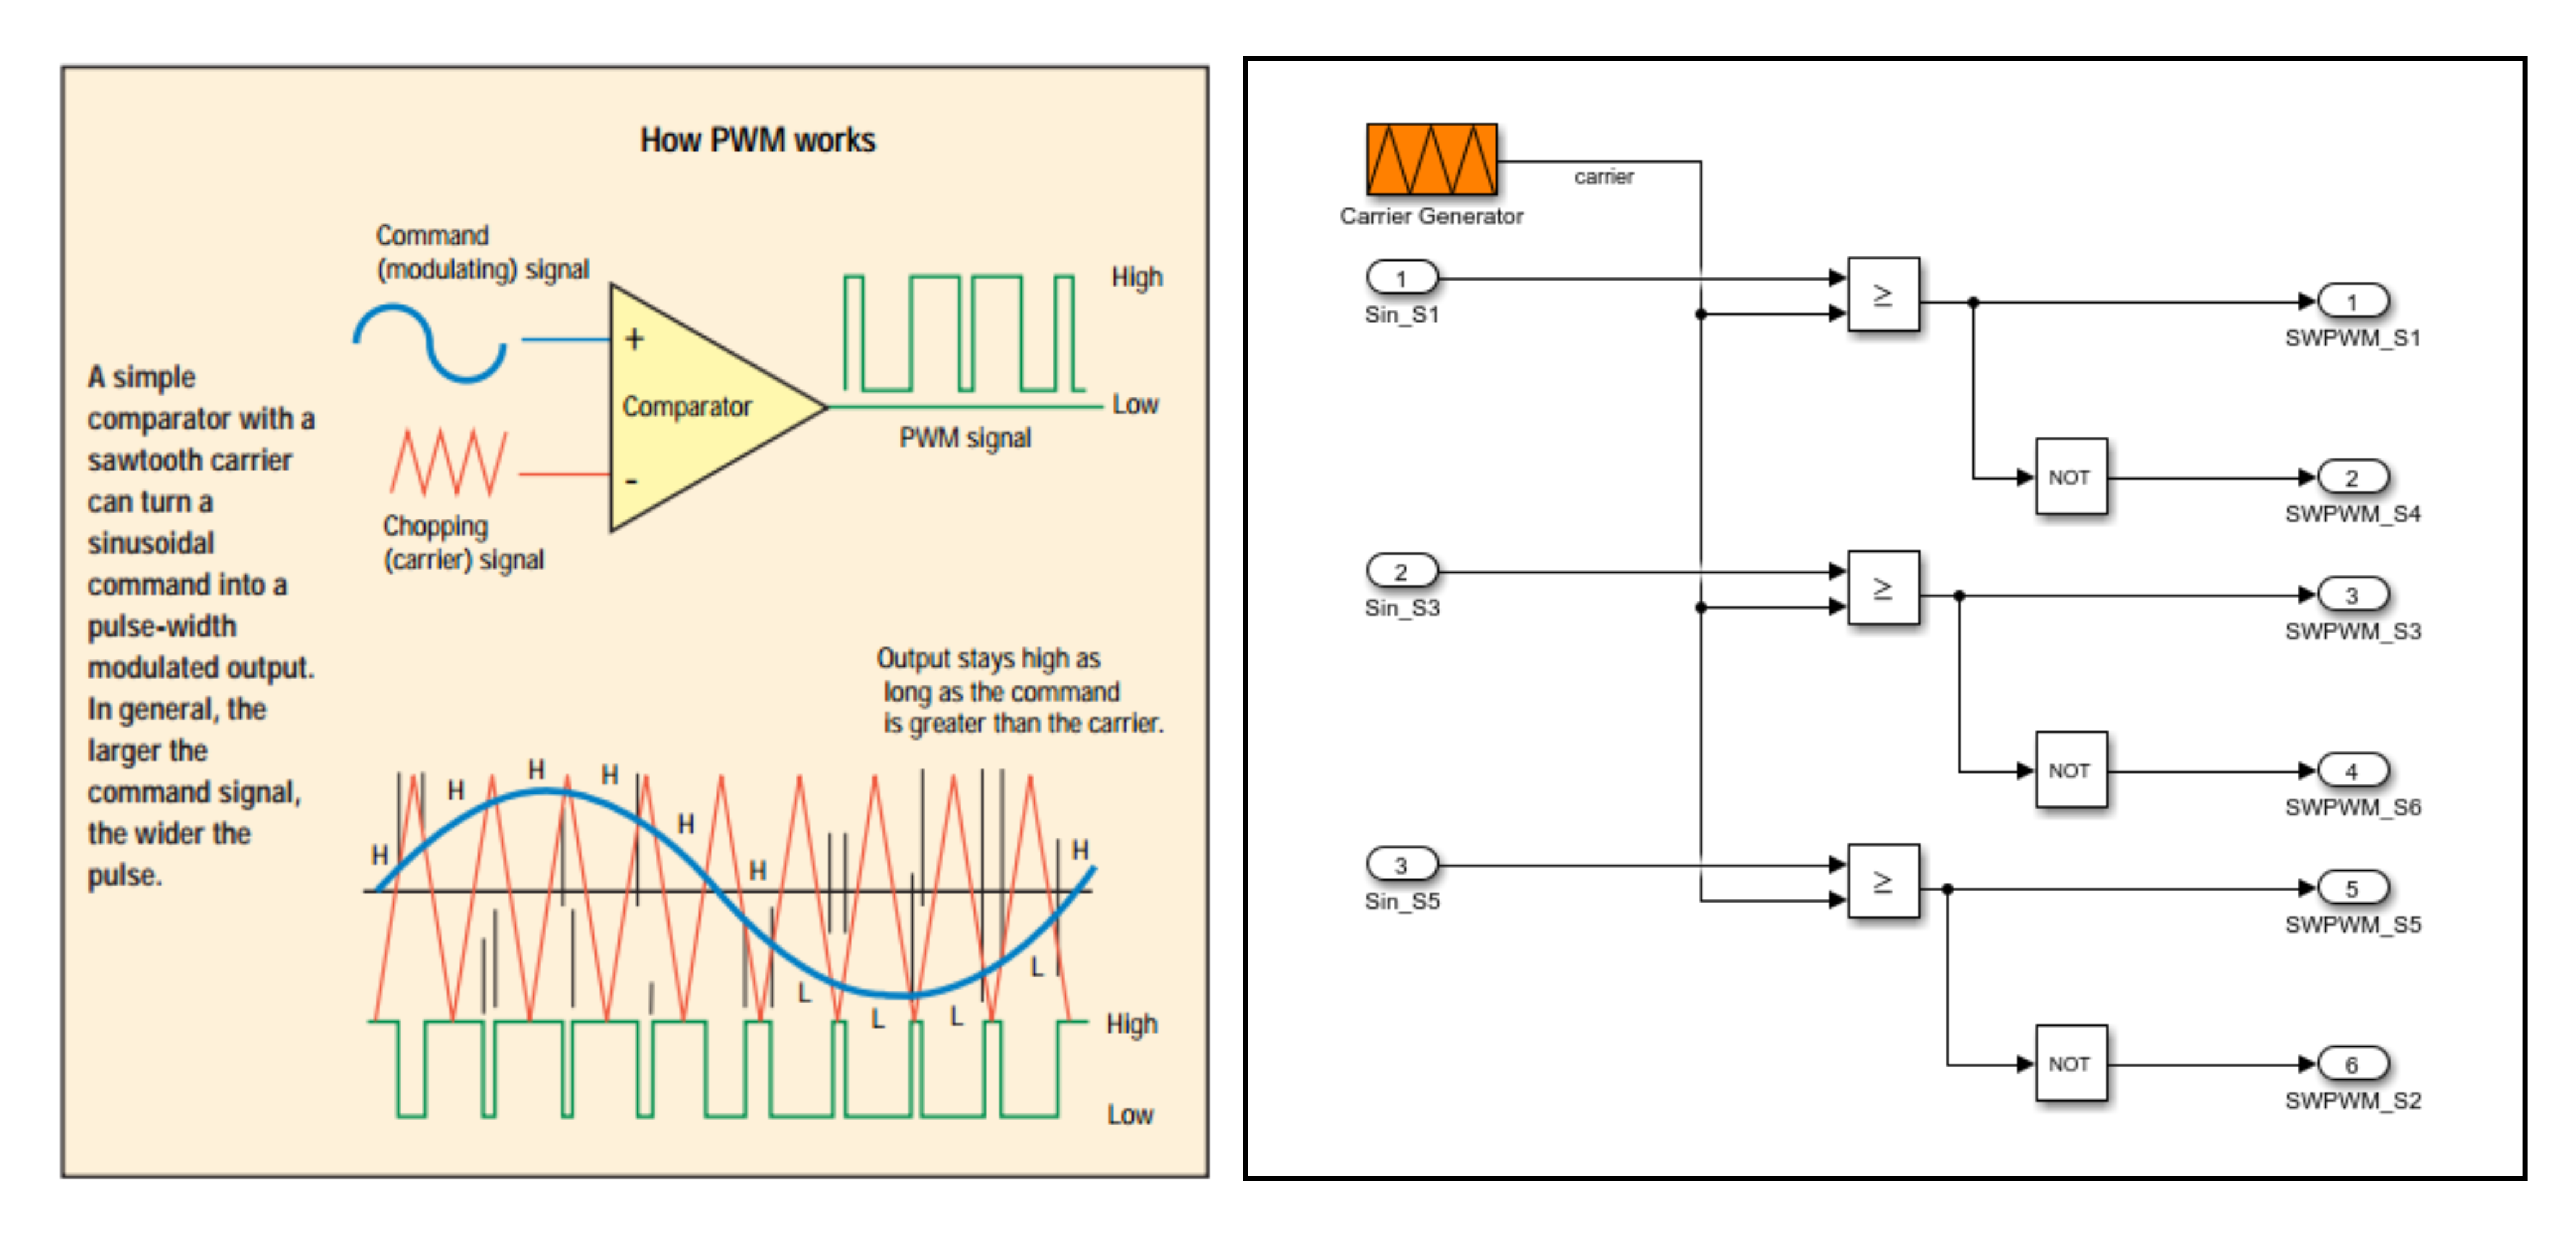
\includegraphics[width=12cm]{PWM_gen}}
					\caption{Szinuszos jelből PWM}		
				\end{figure}
		\pagebreak	
		\subsection{Szimulációs eredemények}
		
			Az inverter vezérlést a szabályozást tekintve "open-loop"-ban teszteltem, a referencia feszültségeket pedig egy szimmetrikus háromfázisú szinuszos jelek alkotják. Paraméterek tekintetében szükséges beállítani az inverter kapcsolási, valamint a térvektor moduláció mintavételi frekvenciáját. 
			\begin{align*}
				& U_{DC} = 400  &&\text{Egyenfeszültség forrás [V]} \\
				& U_{rms} = 230 &&\text{RMS érték [V]} \\
				& U_{peak} = U_{rms} \cdot \sqrt{2} &&\text{Referencia feszültségek amplitúdója [V]} \\
				& f_{fund} = 50 &&\text{Alap harmonikus frekvencia [Hz]} \\
				& \omega = 2 \cdot \pi \cdot f_{fund} &&\text{Szögsebesség [rad/s]}\\
				& f_{samp} = 1000 &&\text{Impulzusszélességek mintavételi frekvenciája [Hz]}\\
				& f_{sw} = 300 &&\text{Inverter kapcsolási frekvencia [Hz]}\\
				& Ts_{sim} = 1e-7 &&\text{Szimuláció/fizikai modellek solverének mintavételi ideje [s]}\\	
			\end{align*}
			\begin{align}
				& U_{U_{REF}} = U_{peak} \cdot sin \Pbracket{\omega \cdot t} \\
				& U_{V_{REF}} = U_{peak} \cdot sin \Pbracket{\omega \cdot t-  \frac{4\pi}{3}} \\
				& U_{W_{REF}} = U_{peak} \cdot sin \Pbracket{\omega \cdot t -  \frac{8\pi}{3}}  
			\end{align}
				
			\begin{figure}[!htb]
				\centering
				\label{Simulink SVPWM}
				\tcbox{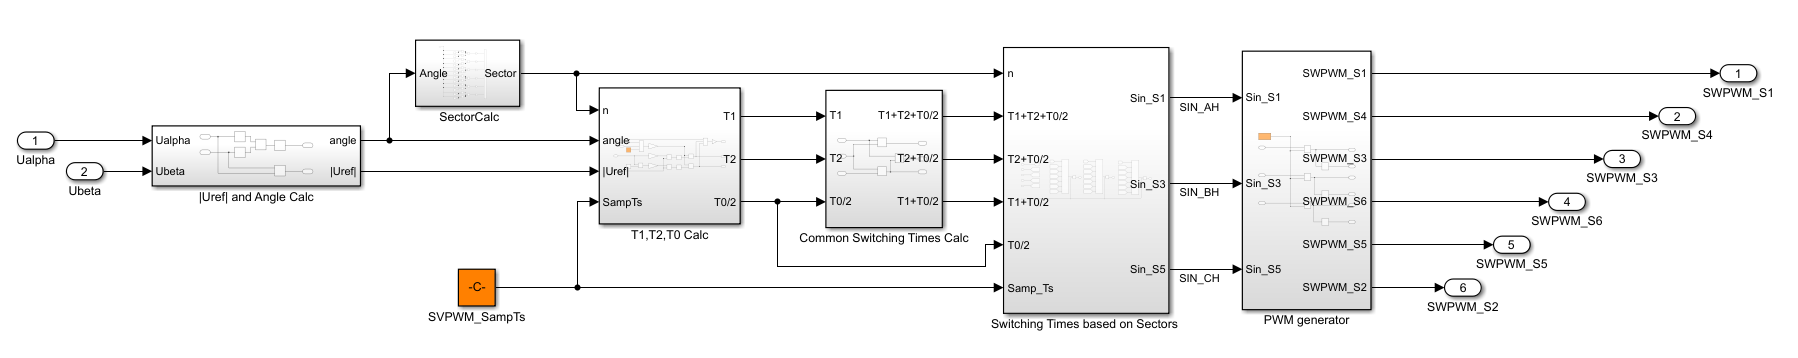
\includegraphics[width=14cm]{svpwm_sim}}
				\caption{SVPWM implementációja}		
			\end{figure}
			
			Az inverter modellben lévő differenciálegyenletek közelítése Forward - Euler módszerrel történik.
			\begin{align}
				& y_n = y_{n-1} + h \cdot f(x_{n-1},y_{n-1}) 
			\end{align}
			\pagebreak
			\begin{figure}[!htb]
				\centering
				\label{simscape_inv}
				\tcbox{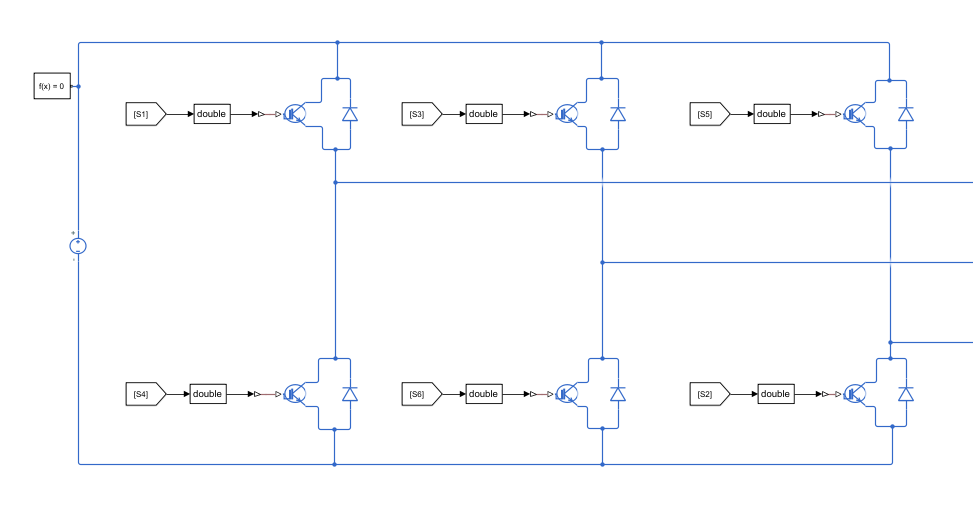
\includegraphics[width=10cm]{simscape_inv}}
				\caption{Kétszintű inverter modell}		
			\end{figure}
			
			A PWM-ek képzéséhez, a vivőjelet egy szimmetrikus háromszögjelet ismétlő szekvenciával valósítottam meg, melynek periódus ideje megegyezik az inverter kapcsolási frekvenciájának periódusidejével. A háromszög jel $ \frac{T_{sw}}{2} $ időközönként 0 és 1 értéket.	
			Az inverter kapcsolóit az alábbiak alapján működtetjük:
			\begin{itemize}
				\item Ha a kitöltés értéke nagyobb egyenlő, mint a vivőjel a kimenet 0, akkor az adott kitöltéshez tartozó kapcsoló nem vezet.
				\item Ha a kitöltés értéke kisebb , mint a vivőjel akkor a kimenet 1, akkor az adott kitöltéshez tartozó kapcsoló vezet. 
			\end{itemize}
			
			\begin{figure}[!htb]
				\centering
				\label{PWM_comp}
				\tcbox{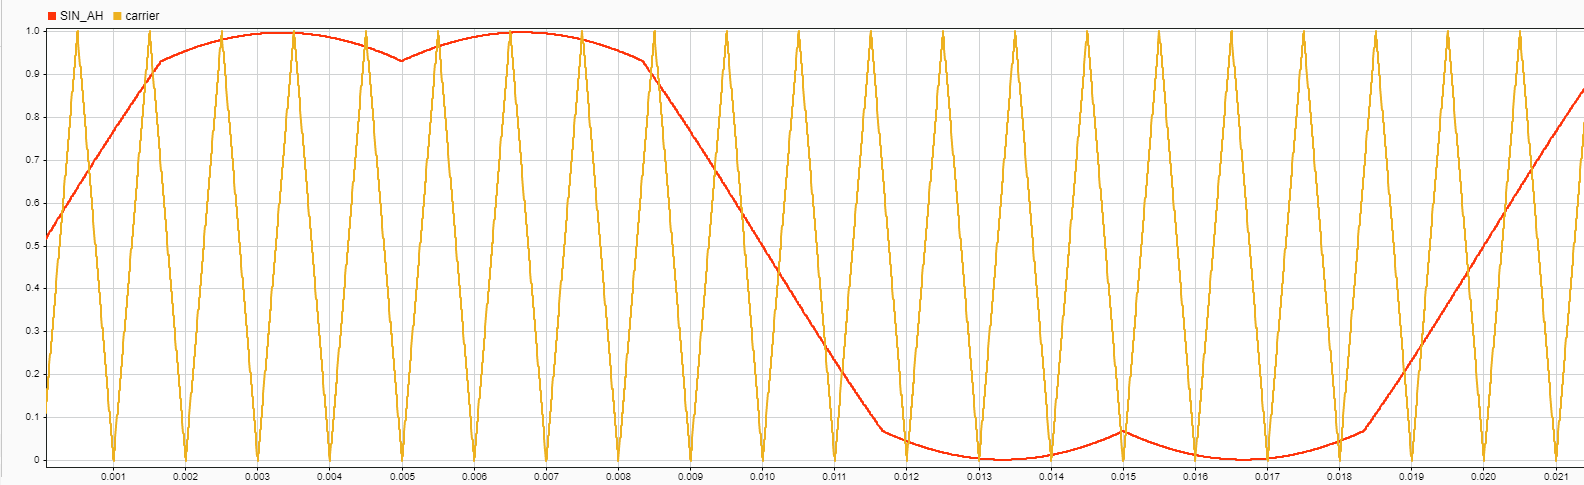
\includegraphics[width=14cm]{spwm_duty}}
				\caption{ Vivőjel és moduláló jel komparálása}		
			\end{figure}
			
			A fázisfeszültségeket az inverter negatív sínjéhez mérve, jól látható $-U_{DC} $ és a $ U_{DC} $ között kapcsolgatunk, valamint jellegükben megegyezőek kapcsolók a PWM jelével.
			\begin{figure}[!htb]
				\centering
				\label{PWM_comp}
				\tcbox{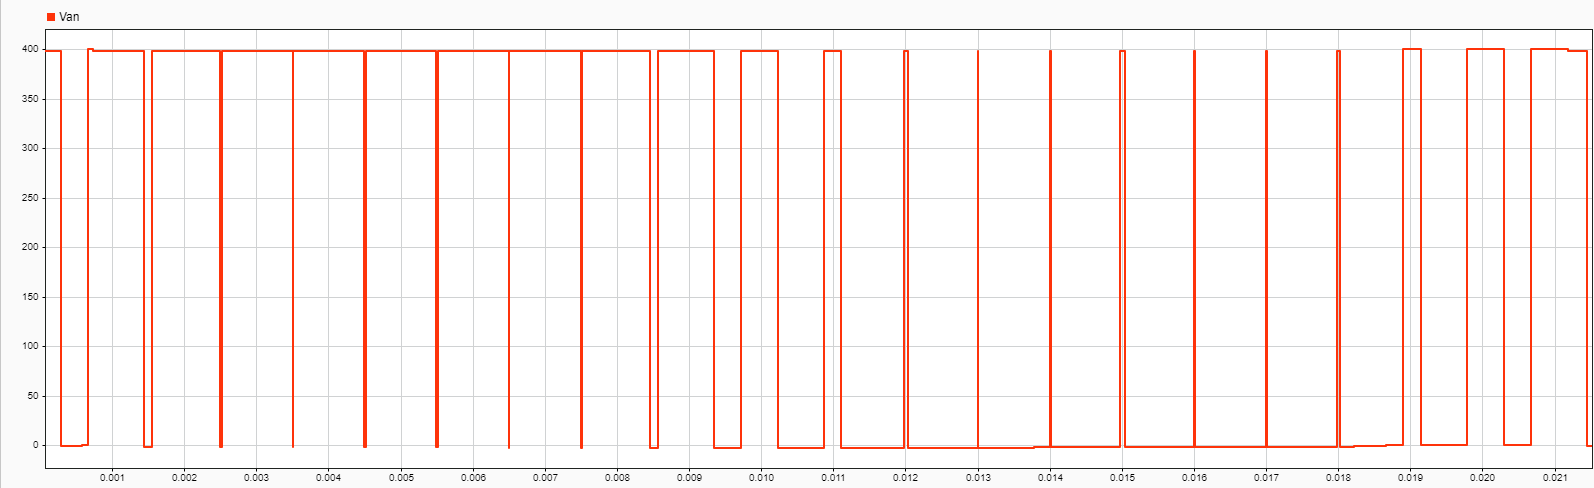
\includegraphics[width=14cm]{spwm_pwm}}
				\caption{ Inverter fázisfeszültsége egy fázison}		
			\end{figure}
			
%	\section{Rotor flux estimation in stator oriented stationary frame ($\alpha - \beta $)using voltage model}


	
%		\subsection{Control scheme from MathWorks}
		
%			\begin{figure}[!htb]
%				\centering
%				\label{fig:flux_estimation }
%				\tcbox{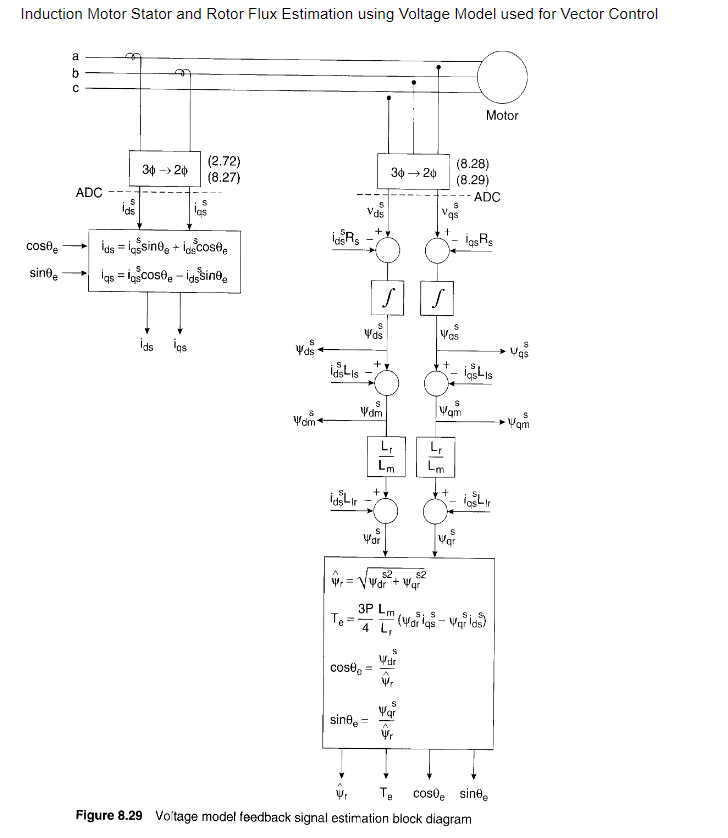
\includegraphics[width=7cm]{flux_estimation}}		
%			\end{figure}
			
%		\subsection{Clarke transformation ($u_{\alpha s} $ , $u_{\beta s}$ , $i_{\alpha s }$ , $i_{\beta s}$ )}
			
%			\[
%			T[ \alpha \beta ] = \frac{2}{3} \cdot
%			\begin{bmatrix}
%				1 & -\frac{1}{2} & -\frac{1}{2} \\
%				0 & \frac{\sqrt{3}}{2} & -\frac{\sqrt{3}}{2}
%			\end{bmatrix}
%			\]
			
			
%			\begin{itemize}
%				\item Voltages :  $u_{\alpha s}$ , $u_{\beta s}$
%				\item Currents :  $i_{\alpha s }$ , $i_{\beta s}$
%			\end{itemize}
		
%		\subsection{Stator voltage equations ($ u_{\alpha s} $ , $  u_{\beta s} $)}
		
%			\begin{align}
%				& u_{\alpha s} = R_{s} \cdot i_{\alpha s}  + \psi_{\alpha s} \cdot \frac{d}{dt} \\
%				& u_{\beta s} = R_{s} \cdot i_{\beta s}  + \psi_{\beta s} \cdot \frac{d}{dt}
%			\end{align}
		
%		\subsection{Stator flux estimation ($\psi_{\alpha s}$ , $ \psi_{\beta s} $)}
		
%			\begin{align}
%				& \psi_{\alpha s} = \int{(u_{\alpha s} -  R_{s} \cdot i_{\alpha s})\ dt} \\
%				& \psi_{\beta s} = \int{(u_{\beta s} -  R_{s} \cdot i_{\beta s})\ dt} \\
%				& \psi_s  = \sqrt { (\psi_{\alpha s})^2 + (\psi_{\beta s})^2 }
%			\end{align}
				
%		\subsection{Magnetizing flux estimation ($ \psi_{\alpha m} $ , $  \psi_{\beta m} $ )}
		
%			\begin{align}
%				&  \psi_{\alpha m}  = \psi_{\alpha s}  - L_{ls} \cdot i_{\alpha s} = L_{m} \cdot (i_{\alpha s} + i_{\alpha r}) \\
%				&  \psi_{\beta m}  = \psi_{\beta s}  - L_{ls} \cdot i_{\beta s} =L_{m} \cdot (i_{\beta s} + i_{\beta r}) 
%			\end{align}
					
%		\subsection{Rotor flux estimation ($ \psi_{\alpha r} $ , $ \psi_{\beta r} $ )}
			
%			\begin{align}
%				&  \psi_{\alpha r} = L_{m} \cdot i_{\alpha s } + (L_{m} + L_{lr} \cdot i_{\alpha r}) = L_{m} \cdot i_{\alpha s } + L_{r} \cdot i_{\alpha r} \\
%				& \psi_{\beta r} = L_{m} \cdot i_{\beta s } + (L_{m} + L_{lr} \cdot i_{\beta r}) = L_{m} \cdot i_{\beta s } + L_{r} \cdot i_{\beta r}
%			\end{align}

%		\subsection{Expressing $i_{\alpha r}$ , $i_{\beta r}$ from $\psi_{\alpha m}$ ,$\psi_{\beta m}$  magnetizing fluxes and substitute to $\psi_{\alpha r}$ ,$\psi_{\beta r} $  }
		
		
%			\begin{align}
%				& i_{\alpha r} = \frac{\psi_{\alpha m}}{L_{m}} - i_{\alpha s} \\
%				& \psi_{\alpha r} = L_{m} \cdot i_{\alpha s} + (L_{m} + L_{lr} ) \cdot ( \frac{\psi_{\alpha m}}{L_{m}} - i_{\alpha s} ) \\
%				& \psi_{\alpha r} = L_{m} \cdot i_{\alpha s} - L_{m} \cdot i_{\alpha s} - L_{lr} \cdot i_{\alpha s}  + L_r \cdot \frac{\psi_{\alpha m}}{L_{m}} \\
%				& \psi_{\alpha r} =	- L_{lr} \cdot i_{\alpha s}  + L_r \cdot \frac{\psi_{\alpha m}}{L_{m}} \\
%				& \psi_{\alpha r} = \frac{L_{r}}{L_{m}} \cdot \psi_{\alpha m} - L_{lr} \cdot i_{\alpha s} \\
%				& \psi_{\beta r} = \frac{L_{r}}{L_{m}} \cdot \psi_{\beta m} - L_{lr} \cdot i_{\beta s}
%			\end{align}
			
%		\subsection{ Rotor flux magnitude ($ \psi_r $), Rotor flux angle ($\varphi_{\psi_r} $)}
			
%			\begin{align}
%				& \psi_r  = \sqrt { (\psi_{\alpha r})^2 + (\psi_{\beta r})^2 } \\
%				&  \varphi_{\psi_r} = \tanh{\frac{ \psi_{\beta r}}{ \psi_{\alpha r}}}
%			\end{align} 
	\pagebreak
	\section{Rotorfluxus becslő tervezése}
	
		Mezőorientált szabályozásban a visszacsatolt méréseket a D-Q forgó koordináta-rendszerbe transzformált motor áramok, valamint az álló és forgó koordináta rendszer közötti szög képezi. A fluxus hardveres mérése csak nagyon költségesen kivitelezhető, ezért többnyire ezt számolni szokás. Mezőorientált szabályozásban a koordináta rendszert úgy  orientáljuk, hogy a rotorfluxus vektor megegyezzen a koordináta rendszer fluxusképző komponensének irányával, tehát a rotorfluxus vektor nyomatékképző komponense 0 legyen. Az így kapott szög a mágnes pozícióját adja meg a  D-irányhoz képest. A rotorfluxus szög meghatározásához történhet az állórészhez tartozó fázisáramok, vagy a fázisfeszültségek mérésének felhasználásával. Attól függően, hogy a számításhoz a rotor mechanikai szögsebességét mérjük vagy becsüljük beszélhetünk direct és indirect megvalósításról. Az autóiparban többnyire a szenzoros megvalósítást preferálják, ugyanis biztonság tekintetében a sensorless megvalósítás drágább és több fejlesztést igényel. Az állórész áramai alapján történő becslés pontosabb mintha feszültség alapján becsülnénk. A pontosság és biztonságkritikai szempontok miatt az implementációban áramalapú fluxusbecslőt alkalmaztam, amely költségesebb, ugyanis felhasználja mechanikai szögsebességet, ami szükségessé teszi resolver használatát. A kontroll modellben a fluxus szög bemenete lesz az invertervezérlés referencia feszültségeit szolgáltató Inverz Park transzformációnak, valamint az áramszabályzók referencia jelét előállító Park transzformációnak. A Park transzformáció a két fázisú mennyiségeket álló (időfüggő) koordináta-rendszerből két fázisú forgó (időfüggetlen) koordináta rendszerben transzformálja. A kontrol alapját ez a transzformáció képezi, ugyanis minden mennyiséget fel tudunk bontani nyomatékot és fluxust képző komponensekre, melyek DC jellegű mennyiségek. A transzformáció bemenete az $\alpha$-$\beta$ mennyiségek, valamint a fluxusszög. Az Inverz Park transzformáció pont ennek visszaalakítása, tehát két fázisú forgó (időfüggetlen) koordináta rendszerből két fázisú álló (időfüggő) koordináta rendszerbe transzformál.
		
		\begin{figure}	
			\begin{equation*}
				\renewcommand\arraystretch{1.5} % Adjust the vertical spacing
				\begin{bmatrix}
					\cos(\omega t) & \sin(\omega t)\\
				   -\sin(\omega t) & \cos(\omega t)
				\end{bmatrix}
				\begin{bmatrix}
					U_{\alpha}\\
					U_{\beta } 
				\end{bmatrix}
				=
				\begin{bmatrix}
					U_{D} \\
					U_{Q}
				\end{bmatrix}
			\end{equation*}
		\caption{Park transzformáció}
	 	\end{figure}
	 	
	 	\begin{figure}	
	 		\begin{equation*}
	 			\renewcommand\arraystretch{1.5} % Adjust the vertical spacing
	 			\begin{bmatrix}
	 				\cos(\omega t) & -\sin(\omega t)\\
	 				\sin(\omega t) &  \cos(\omega t)
	 			\end{bmatrix}
	 			\begin{bmatrix}
	 				U_{D}\\
	 				U_{Q } 
	 			\end{bmatrix}
	 			=
	 			\begin{bmatrix}
	 				U_{\alpha} \\
	 				U_{\beta}
	 			\end{bmatrix}
	 		\end{equation*}
	 		\caption{Inverz Park transzformáció}
	 	\end{figure}
		
		\pagebreak
		A feszültségeket forgó koordináta rendszerben ábrázolva, a rotor oldalról nézzük az állórészt. Az állórész mezőjének szögsebessége ennek tekintetében a slip sebességgel forog. ($ \omega_{slip} = \omega - \omega_{r} $)
		\begin{align}
			& U_{dr} = R_r \cdot i_{dr} + \Psi_{dr} \cdot \frac{d}{dt} - (\omega - \omega_{r}) \cdot \Psi_{qr} = 0 \\
			& U_{qr} = R_r \cdot i_{qr} + \Psi_{qr} \cdot \frac{d}{dt} + (\omega - \omega_{r}) \cdot \Psi_{dr} = 0
		\end{align}
		
		A fluxusbecslő a két fázisú álló koordináta rendszer egyenleteit használja, ahol a stator oldalról nézve az állórész szögsebessége nulla. ($\omega = 0 $)
		\begin{align}
			& U_{r\alpha} = R_r \cdot i_{r\alpha} + \Psi_{r\alpha} \cdot \frac{d}{dt} + \omega_{r} \cdot \Psi_{r\beta} \\
			& U_{r\beta} = R_r \cdot i_{r\beta}  + \Psi_{r\beta}  \cdot \frac{d}{dt} - \omega_{r} \cdot \Psi_{r\alpha} 	
		\end{align}	
		
		Alpha-irányban  $ \frac{L_m \cdot R_r}{L_r} \cdot i_{s\alpha} $, béta-irányban  $ \frac{L_m \cdot R_r}{L_r} \cdot i_{s\beta} $ adunk mindkét oldalhoz. Ennek eredményeképpen mindkét irányhoz tartozó rotorfluxus kifejezhetővé válik. Az egyenletek az alábbi formára egyszerűsödnek.
		\begin{align}
			& \Psi_{r\alpha} \cdot \frac{d}{dt} +  \frac{R_r}{L_r} \cdot (L_m \cdot i_{s\alpha} + L_r \cdot i_{r\alpha}) + \omega_r \cdot \Psi_{r\beta}  = \frac{L_m \cdot R_r}{L_r} \\
			& \Psi_{r\beta} \cdot \frac{d}{dt} +  \frac{R_r}{L_r} \cdot (L_m \cdot i_{s\beta}  + L_r \cdot i_{r\beta} ) - \omega_r \cdot \Psi_{r\alpha} = \frac{L_m \cdot R_r}{L_r}\\
			& \Psi_{r\alpha} = L_m \cdot i_{s\alpha}   + L_r  \cdot i_{r\alpha} \\
			& \Psi_{r\beta} = L_m \cdot i_{s\beta}  + L_r  \cdot i_{r\beta} 
		\end{align}
		A (55) és (56)-ot behelyettesítve (53) és (54)-be az alábbi formát kapjuk:
		\begin{align}
			& \Psi_{r\alpha} \cdot \frac{d}{dt} +  \frac{R_r}{L_r} \cdot \Psi_{r\alpha} + \omega_r \cdot \Psi_{r\beta} = \frac{L_m \cdot R_r}{L_r} \cdot i_{r\alpha}  \\
			& \Psi_{r\beta} \cdot \frac{d}{dt} +  \frac{R_r}{L_r} \cdot \Psi_{r\beta} - \omega_r \cdot \Psi_{r\alpha} = \frac{L_m \cdot R_r}{L_r} \cdot i_{r\beta} 
		\end{align}
		
		Rotorfluxus folytonos időbeli differenciálegyenleteinek felírása alpha és béta irányba:
		\begin{align}
			& \Psi_{r\alpha}\frac{d}{dt} = \frac{L_m}{T_r} \cdot i_{s\alpha} - \omega_r \cdot \Psi_{ry} - \frac{1}{T_r} \cdot \Psi_{r\alpha} \\
			& \Psi_{r\beta} \frac{d}{dt} = \frac{L_m}{T_r} \cdot i_{s\beta} + \omega_r \cdot \Psi_{r\alpha} - \frac{1}{T_r} \cdot \Psi_{r\beta}
		\end{align}
		
		A folytonos idejű differenciálegyenleteket Euler alkalmazásával diszkrét idejűvé alakíthatjuk.
		\begin{align}
			& \Psi_{r\alpha}[k] = \Pbracket {\frac{L_m}{T_r} \cdot i_{s\alpha}[k] - \omega_{r} \cdot \Psi_{r\beta}[k-1] - \frac{1}{T_r} \cdot \Psi_{r\alpha}[k-1]} \cdot T_s + \Psi_{r\alpha}[k-1] \\
			& \Psi_{r\beta}[k] = \Pbracket {\frac{L_m}{T_r} \cdot i_{s\beta}[k] - \omega_{r} \cdot \Psi_{r\alpha}[k-1] - \frac{1}{T_r} \cdot \Psi_{r\beta}[k-1]} \cdot T_s + \Psi_{r\beta}[k-1] 		
		\end{align}
		
	   Rotorfluxus szög és amplitúdó számítása:
		\begin{align}
			& |\Psi_{r}[k]|  = \sqrt{ \Psi_{r\alpha}[k]^2 + \Psi_{r\beta}[k]^2 } 
			& \Theta_{\Psi_r}[k] = \frac{\Psi_{r\beta}[k]}{\Psi_{r\alpha}[k]}
		\end{align}
		\begin{figure}[!htb]
			\centering
			\label{rotorfluxdq}
			\tcbox{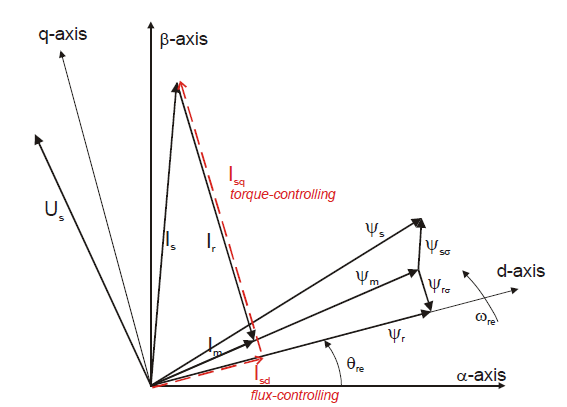
\includegraphics[width=9.7cm]{rotorfluxdq}}
			\caption{ Rotorfluxus vektor ábrázolása}		
		\end{figure}
		
		
	\pagebreak	
	\section{Tesztelés : Sebességszabályozás}
	
	\subsection{Fázis feszültségek visszaalakítása kitöltéssé}
	
	A PWM fázisfeszültségekből megfelelő szűrőméretezéssel visszakaphatjuk a kapcsolók bemenetét képező kitöltési tényezőket. Ezzel tesztelhetjük, hogy az invertervezérlésünknek megfelelő fázisfeszültségekkel gerjesztjük a motort. Hardveresen ezt egy RC körrel tudjuk megvalósítani, amely működése tekintetében egy aluláteresztő szűrőnek feleltethető meg, ahol a filterezett jelet a kapacitás feszültségének méréséből kapjuk.
	
	\begin{align}
		& X_{c} = \frac{1}{\omega \cdot C} = \frac{1}{2 \cdot \pi \cdot f_{fund} \cdot C }
	\end{align}
	
	A kapacitás képletéből adódóan minél kisebb a bemenő feszültségének frekvenciája, a kapacitás reaktanciája annál nagyobb lesz és a rajta eső feszültség csökken. Minél nagyobb a bemenő feszültség frekvenciája, a kapacitás reaktanciája annál kisebb lesz és a rajta eső feszültség növekszik. Ez alapján az RC kör megfeleltethető egy aluláteresztő szűrőnek, amely a vágási körfrekvenciánál kisebb frekvenciájú jelet át engedi, a nagyobb frekvenciás jeleket pedig kiszűri, melyek a Bode-diagram tekintetében a -20dB/dekád meredekségű letörési tartományba esnek. A feszültségmérőt az RC kör negatív pólusa, inverter negatív sínjére van kötve. A vágási körfrekvencia ( $f_{c}$ ) az alapharmonikus frekvencia egy nagyságrenddel nagyobb értéke lesz. A vágási körfrekvencián az erősítés értéke $\frac{1}{\sqrt{2}} $ , az az -3 dB. Ennek megfelelően , azokat a frekvenciákat ,amelyek a vágási körfrekvenciánál egy nagyságrenddel kisebbek ( $f_{fund} $ ), azokat biztosan átengedjük, amelyek pedig egy nagyságrenddel nagyobbak ($f_{sim} $) azokat pedig biztosan kiszűrjük.
	\begin{align}
		& f_{c} = \frac{1}{2 \cdot \pi \cdot R \cdot C}
	\end{align}
	
	\begin{figure}[!htb]
		\centering
		\label{RC}
		\tcbox{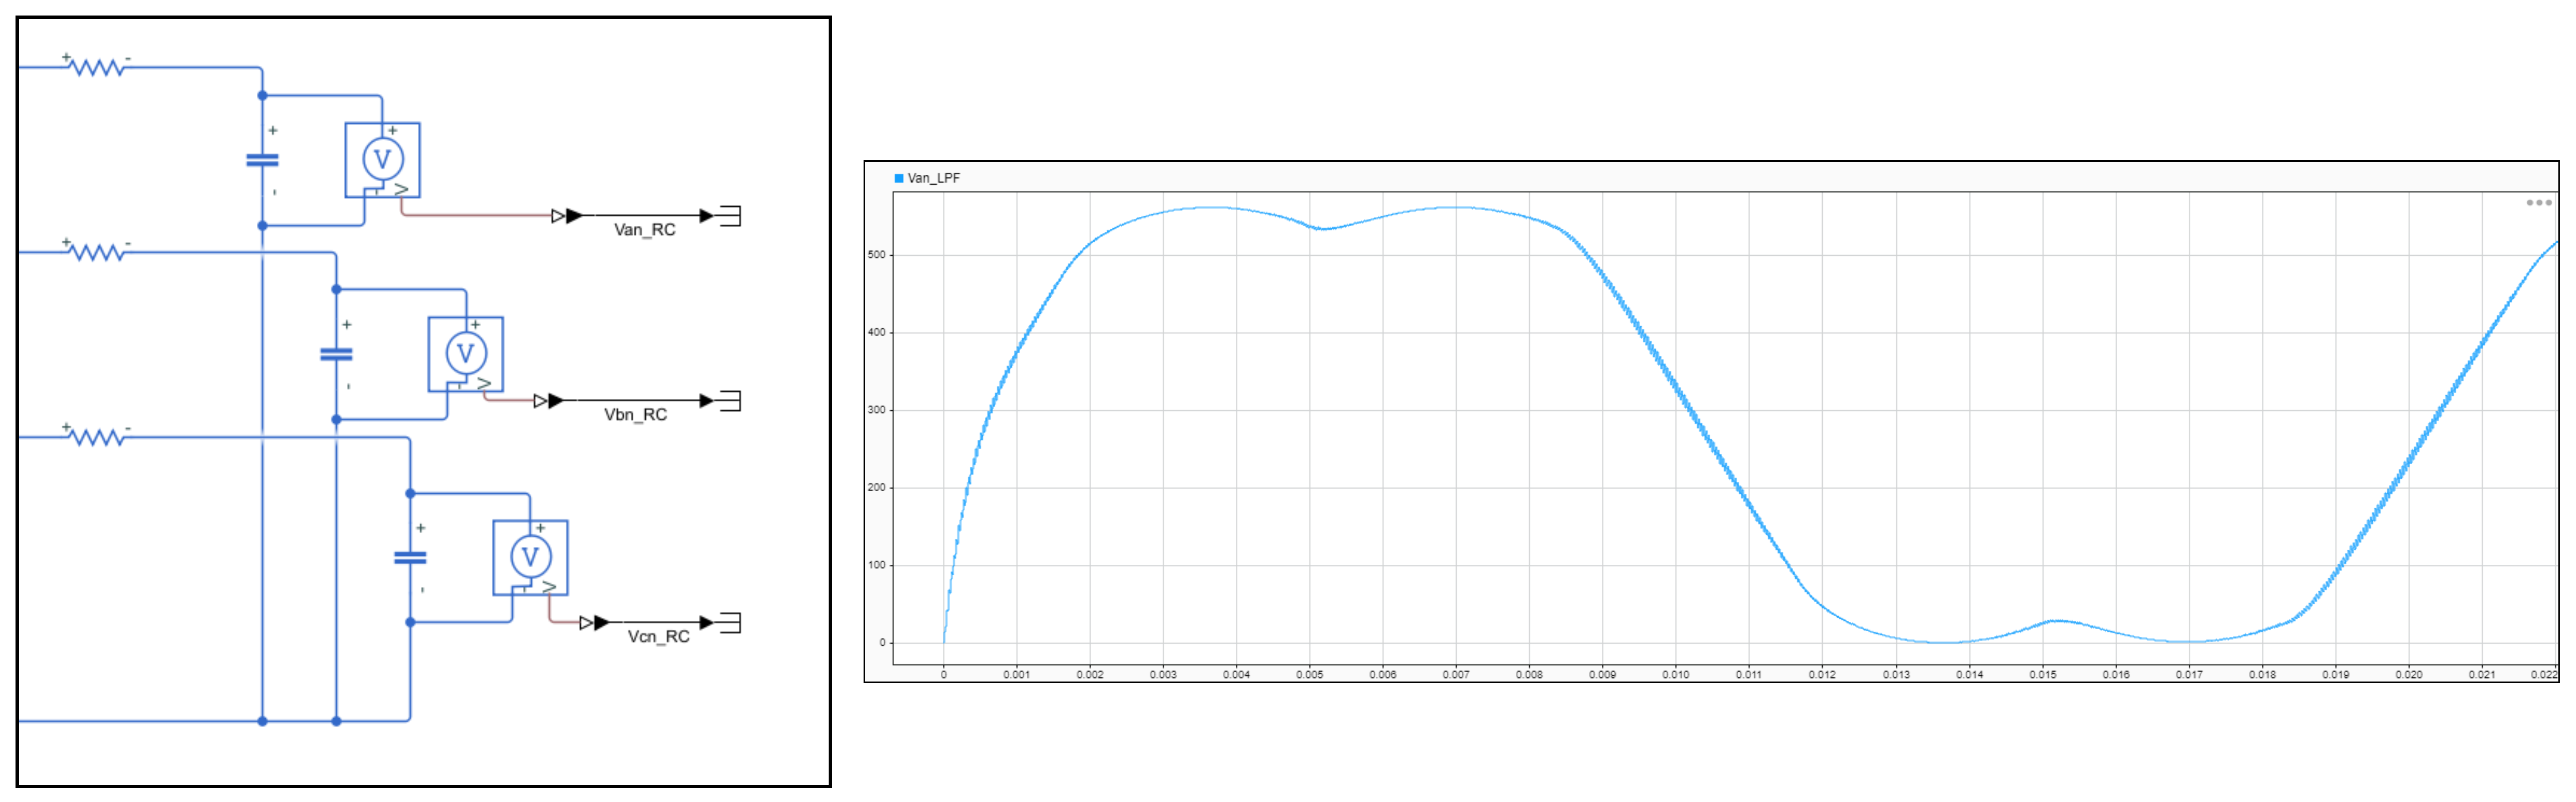
\includegraphics[width=13cm]{RC}}
		\caption{Fázis feszültség mérés RC szűrővel}		
	\end{figure}
	
	\pagebreak
	A kitöltéseket digitális szűrő alkalmazásával is visszakaphatjuk, melyek két fő típusa az IRR és FIR szűrő. A digitális szűrők előnye az RC szűrővel, hogy nem kell plusz áramköri elemeket beiktatni a rendszerbe, és mikrokontroller a mért értékből fázisfeszültségekből szoftveresen el tudja végezni a szűrést. A mérésnél első rendű IIR szűrőt fogok használni, mert számításigénye kevesebb, ezért valós idejű alkalmazásokhoz optimálisabb, mint a FIR szűrő.
	
	\begin{align}
		& y[n] = a_{1} \cdot y[n-1] + b_{0} \cdot u[n]  
	\end{align}
	
	\begin{itemize}
		\item $a_{1}$ , $b_{0}$  : feedback/feedforward együtthatók
		\item $ u[n] $  : bemeneti jel 
		\item $ y[n] $  : kimeneti jel 
		\item $ y[n-1] $ : visszacsatolt kimeneti jel 
	\end{itemize}
	
	Aluláteresztő szűrőként alkalmazva az egyenlet átrendezhető úgy, hogy csak egy darab szűrőegyütthatónk legyen:
	
	\begin{itemize}
		\item $ \alpha $: szűrőegyüttható 
		\item $ a_{1} = 1 - \alpha $
		\item $ b_{0} = \alpha $
	\end{itemize}
	
	\begin{align}
		& y[n] = (1 -\alpha) \cdot y[n-1] + \alpha \cdot u[n] \\
		& y[n] = (u[n] - y[n-1] ) \cdot \alpha + y[n-1]
	\end{align}
	
	\begin{figure}[!htb]
		\centering
		\label{IIR_sim}
		\tcbox{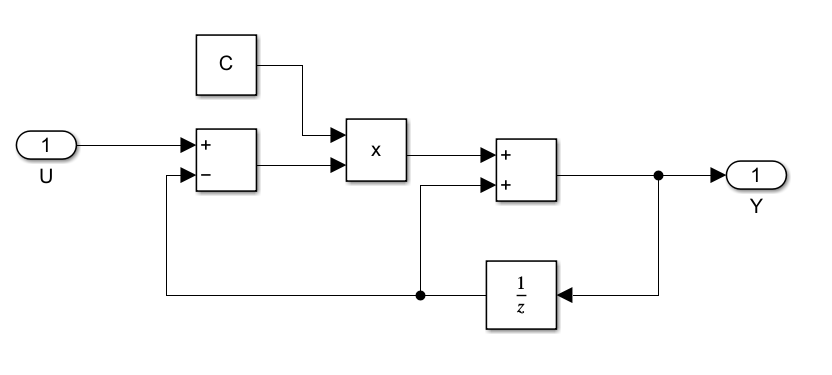
\includegraphics[width=12cm]{IIR_sim}}
		\caption{ IIR aluláteresztő szűrő}		
	\end{figure}
	
	\subsection{Optimális szűrőegyüttható számolása aluláteresztő IRR szűrőhöz  }
	
	Az tervezett vágási körfrekvenciához tartozó szűrőegyüttható ( $\alpha$ ) meghatározásához szükséges felírni a folytonos idejű átviteli függvényt a komplex frekvenciatartományon (Y:erősítés - X:frekvencia). Folytonos időbeli differenciálegyenlet diszkrét idejű átviteli függvényét Laplace transzformációval, diszkrét idejű differenciaegyenlet diszkrét idejű átviteli függvényét Z-transzformációval tudjuk meghatározni. A fenti (1)-es egyenlet diszkrét formában van megadva. Ez alapján Z-transzformációval felírjuk a diszkrét idejű átviteli függvényt, meghatározzuk a diszkrét idejű átviteli függvényt, majd folytonossá alakítjuk.
	A Z-transzformáció elsődleges szabálya:
	\begin{align}
		& y[n-k] = Y(z) \cdot z^{-k}
	\end{align}
	
	Ez alapján az IRR szűrő differenciaegyenletének mindkét oldalán előállítjuk Z-transzformáltat, majd rendezzük:
	
	\begin{align}
		& Y(z) = (1-\alpha) \cdot Y(z) \cdot z^{-1} + \alpha \cdot X(z) \\
		& Y(z) \cdot (1 - (1-\alpha) \cdot z^{-1} )  = X(z) \cdot \alpha
	\end{align}
	
	Az átviteli függvényt ( $ G(z) $ ) a Z-transzformált kimeneti függvényének ( $ Y(z) $ )  és bemeneti függvényének ( $ X(z) $ ) hányadosaként határozzuk meg, és az alábbi formában írható fel:
	\begin{align}
		& G(z) = \frac{Y(z)}{X(z)} = \frac{\alpha}{(1 - (1-\alpha) \cdot z^{-1}} 
	\end{align}
	
	A diszkrétből folytonos időbeli átviteli függvény felírásához k-ad rendű Z-transzformált egyenlete:
	\begin{align}
		& z^{-k} = e^{-k \cdot j \theta} = \cos{\theta} - j \cdot k \cdot \sin{\theta}
	\end{align}
	
	Ez alapján az IRR szűrő folytonos időbeli átviteli függvénye:
	\begin{align}
		& G(\theta) = \frac{\alpha}{ (1 - (1-\alpha) \cdot ( \cos{\theta} - j \cdot \sin{\theta} ) }
	\end{align}
	
	Theta a normalizált szögsebesség:
	\begin{align}
		& \theta = \omega \cdot T = 2 \pi f T = 2 \cdot \pi \cdot \frac{f_0}{f_s} 
	\end{align}
	
	Ahogy az analóg szűrőknél, úgy itt is úgy tervezzük a szűrőt, hogy a vágási körfrekvenciánál mérhető erősítésének $ \frac{1}{\sqrt{2}} $ kell lennie, ami  $ 20 \cdot \log(\frac{1}{\sqrt{2}}) = -3 $ dB-nek felel meg. Ez alapján az átviteli függvény értéke egyenlő lesz $ \frac{1}{\sqrt{2}} $:
	
	\begin{align}
		& \frac{1}{\sqrt{2}} = \frac{\alpha}{ (1 - (1-\alpha) \cdot ( \cos{\theta} - j \cdot \sin{\theta} ) }
	\end{align}
	
	Az egyenlet átrendezhető:
	\begin{align}
		& \theta = \arccos\Pbracket{\frac{\alpha^2 + 2\alpha - 2}{ 2(\alpha -1 )}}
	\end{align}
	
	$\alpha$-t a következő módon tudjuk kifejezni:
	\begin{align}
		& \cos(\theta) = \cos\Pbracket {\arccos\Pbracket{\frac{\alpha^2 + 2\alpha - 2}{ 2(\alpha -1 )}}} \\
		& \cos(\theta) = \frac{\alpha^2 + 2\alpha - 2}{ 2(\alpha -1 )} = \frac{\alpha^2 + 2\alpha - 2}{ 2\alpha - 2} \\
		& \cos(\theta) - 1 = \frac{\alpha^2 }{ 2\alpha - 2 } \\
		& c = \cos(\theta) \\
		& (2\alpha -2) \cdot (c - 1) = \alpha^2 \\
		& -\alpha^2 + (2c-2) \cdot \alpha -(2c-2) \\
		& \alpha_1,\alpha_2 =\frac{-(2c-2) \pm \sqrt{(2c-2)^2 - 4 \cdot -1 \cdot -(2c-2)}}{-2}	
	\end{align}
	
	A másodfokú egyenlet végeredménye lehet komplex szám is, ezért a szűrőegyütthatónak az $ |\alpha| $ értéket tekintjük.
	\newline Alpha kritériuma, hogy 0 és 1 közé essen. Mivel optimális szűrőegyütthatót keresünk ezért, ha a fenti két feltétel teljesül a kisebb $ \alpha $ értéket választjuk.
	
	\begin{figure}[!htb]
		\centering
		\label{script}
		\tcbox{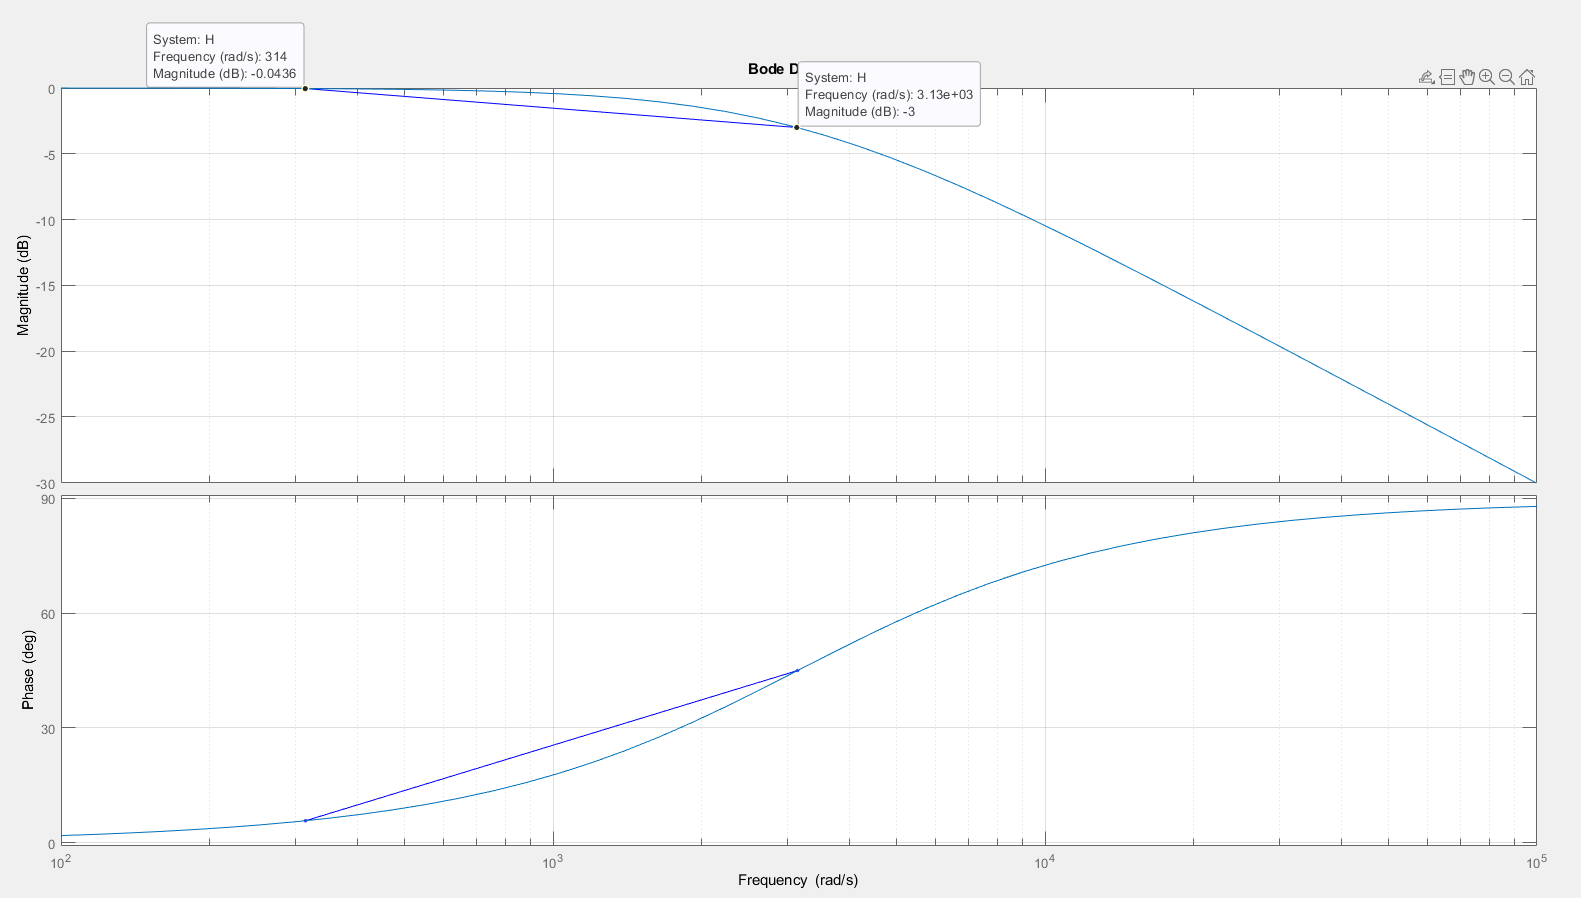
\includegraphics[width=14cm]{bode}}
		\caption{ Bode diagram}		
	\end{figure}

	\begin{itemize}
		\item  $ \omega_f $ -nél erősítés : -0.0436 Db
		\item  $ \omega_c $ -nél erősítés : -3 Db
		\item  $ \omega_s $ -nél erősítés : $ \approx$ -40 Db 
	\end{itemize}
	
	A Z - transzformáció, mellett alkalmazhatunk közelítést is a vágási körfrekvencia kiszámolására:
	\begin{align}
		& \alpha = \frac{2 \cdot \pi \cdot T_s \cdot f_c }{2 \cdot \pi \cdot T_s \cdot f_c + 1}
	\end{align}
	
	\subsection{U/f control}
		
		Az U/f control, vagyis feszültség/frekvencia kontroll a skalár kontrollokhoz tartozik. A szabályozás során  az inverter fázisfeszültségei amplitúdójának és frekvenciájának változtatásával arányukat nem változtatjuk, ennek megfelelően a kialakult rotorfluxus konstans értékre áll be és a motor mechanikai szögsebessége állandósulni fog. Ez lehetővé teszi a motor sebességszabályozását. A szabályozás open-loop és closed loop-ban is megvalósítható. Closed-loop esetben a slip sebességet csatoljuk vissza, open loop esetben nincs visszacsatolás és a mechanikai szögsebességet tekintjük a szinkron sebességnek. Szakdolgozatomban az open-loop megvalósítást implementáltam, és az invertervezérlés funkcióinak tesztelésére használtam. A komponens építéséhez szükséges tudni a motor nominális feszültségét és frekvenciáját. A nominális feszültség a maximális feszültségnek tekinthető. Nulla frekvenciánál a feszültség nem nulla, ugyanis a stator oldali ellenálláson esik valamekkora feszültség. Koordináta rendszerben ábrázolva a vertikális tengelyen a frekvencia, horizontálisan a feszültséget ábrázoljuk. Minden frekvenciához tartozik egy feszültség amplitúdó érték. A nulla frekvencia és nominális frekvencia értékhez tartozó pontokat összekötjük, így egy egyenest kapunk, melynek meredeksége állandó, ezzel biztosítva az U/f arány megtartását. Ahhoz, hogy az invertervezérlésünk bemeneteit megkapjuk, az amplitúdó mellett szükséges az a referencia feszültség aktuális szögének meghatározása, melyet $ -\pi/2 $ és $ \pi/2 $ közé érdemes beszorítani. A működés tekintetében a motort mindkét irányba tudjuk forgatni, melyet az implementáció során a referencia frekvencia érték előjeléből tudunk meghatározni, és a kiszámolt feszültség amplitúdó irányát határozza meg. A nominális frekvenciát elérve, amely a field-weakening pont-nak is tekinthető, a frekvenciát növelve az amplitúdó már nem növelhető tovább, tehát ezen érték elérése után az feszültség amplitúdó a maximális értéken marad. A frekvencia tartományt érdemes úgy megválasztani, hogy a nominális frekvencia kétszerese legyen, ugyanis a motor sebessége nem növelhető minden határon túl.
		
		\begin{figure}[!htb]
			\centering
			\label{uf}
			\tcbox{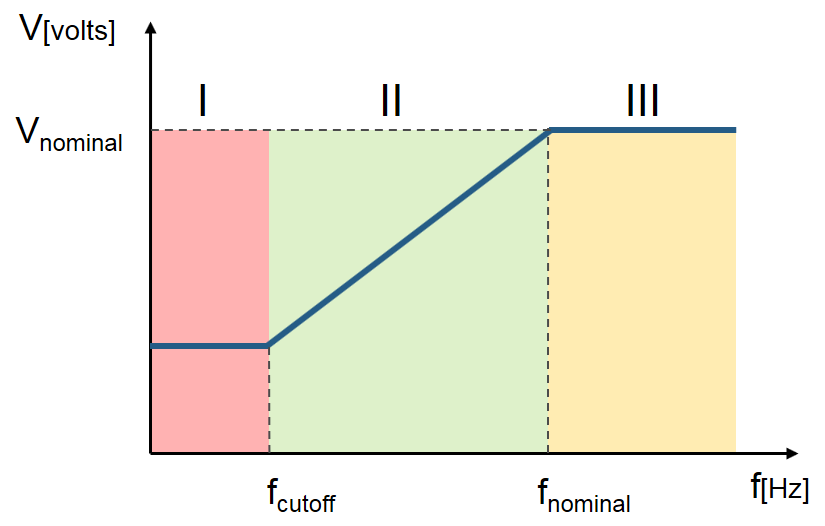
\includegraphics[width=8.5cm]{uf}}
			\caption{ U/f karakterisztikája}		
		\end{figure}
		
		A karakterisztikát három részre tudjuk osztani. Az I. tartományban csak a stator oldali ellenálláson esik feszültség, a tényleges forgási sebesség elhanyagolhatónak tekinthető ( 0 - 5Hz ). A II. tartomány lineárisnak tekinthető, melyben a maximális frekvencia értéke megegyezik a motor nominális frekvenciájával ( 5 - 60Hz ). A III. rész a mezőgyengítési tartomány, ahol már csak a frekvencia növelhető (60 - 120 Hz ). A lineáris tartományban a feszültség meghatározása az egyenes egyenletéből történik ($f_{cutoff} = f_{min}$).
		\begin{align}
			& y = mx + b 
			& U_{amp} = \frac{U_{nom} - U_{min}}{f_{nom} - {f_{min}}}\cdot (f_{ref} -f_{min} ) + U_{min}
		\end{align}
		A szöget, a szögsebesség integrálásából kapjuk, melyre Forward - Euler-t alkalmaztam.
		\begin{align}
			& \Theta[k] = 2 \cdot \pi \cdot f_{ref} \cdot T_s + \Theta[k-1]
		\end{align}
		\begin{figure}[!htb]
			\centering
			\label{uf_ang}
			\tcbox{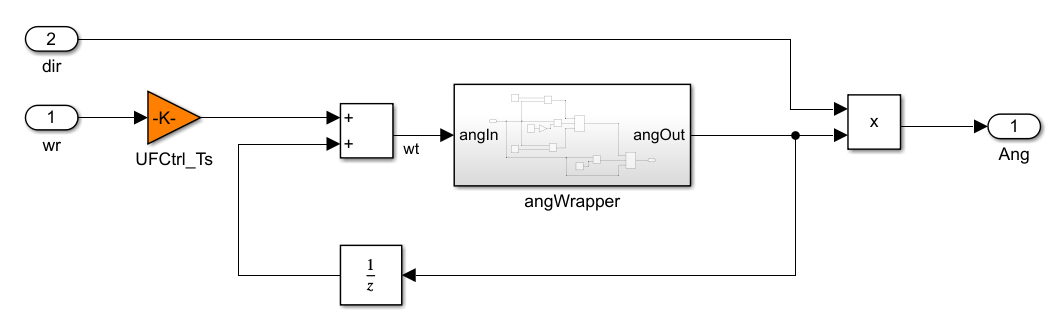
\includegraphics[width=10.7cm]{uf_ang}}
			\caption{ Szög meghatározása}		
		\end{figure}
		
		Az amplitúdó és szög meghatározása után, több fajta módon lehet a fázisfeszültségeket legenerálni, számolhatunk három fázisra, $\alpha - \beta$ és D - Q koordináta-rendszerben. Három fázisra megadva a feszültségek az alábbi módon írhatóak fel.
		
		\begin{align}
			& U_U = U_{amp}  \cdot \sin \Pbracket{ \Theta } \\
			& U_V = U_{amp}  \cdot \sin \Pbracket{ \Theta + \frac{-2\pi}{3}} \\
			& U_W = U_{amp}  \cdot \sin \Pbracket{ \Theta + \frac{2\pi}{3}}
		\end{align}
		
		A tesztelés folyamán 0 - 120 Hz közötti frekvenciatartományon, a frekvencia bemenetet egy lépcsős jel képzi, amely 20 Hz-ként vált. A cél a U/f kontroll a és rotorfluxusbecslő kimeneteinek összehasonlítása a motoron mért értékekkel. A motoron mérhető a mechanikai szögsebesség, valamint az $\alpha - \beta$ irányú rotorfluxus, melyek segítségével az amplitúdó és szög egyszerűen számolható.
	
		\begin{figure}[!htb]
			\centering
			\label{uf_wm}
			\tcbox{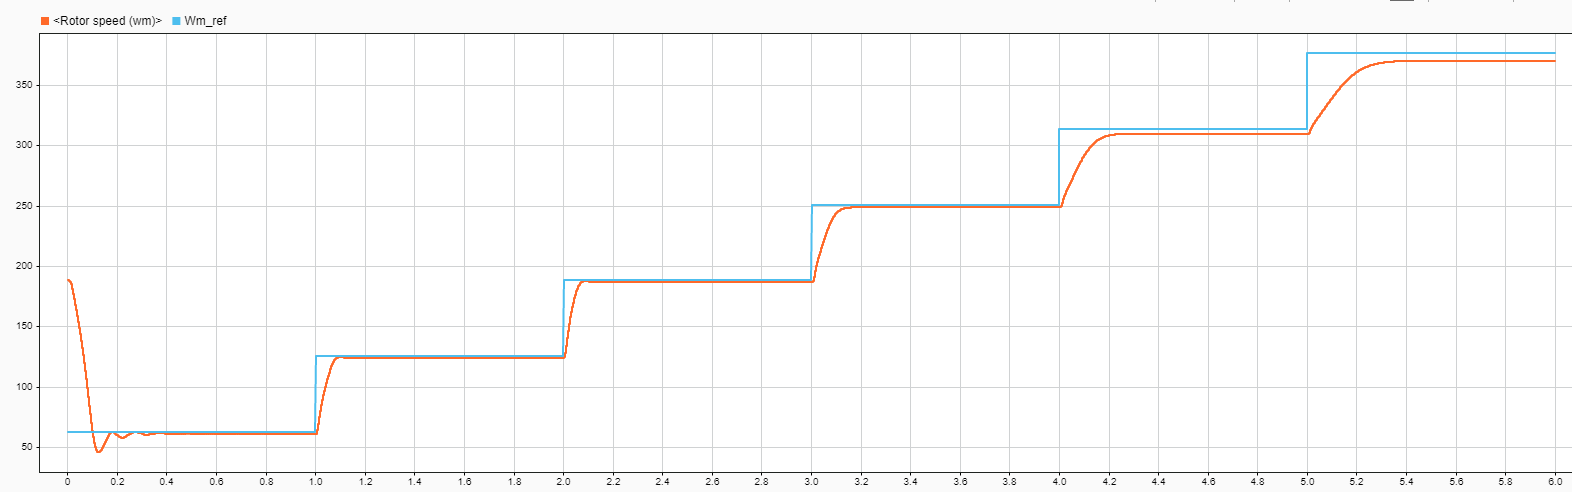
\includegraphics[width=14cm]{uf_wm}}
			\caption{ Sebesség összehasonlítása}		
		\end{figure}
		
		\begin{figure}[!htb]
			\centering
			\label{uf_flux}
			\tcbox{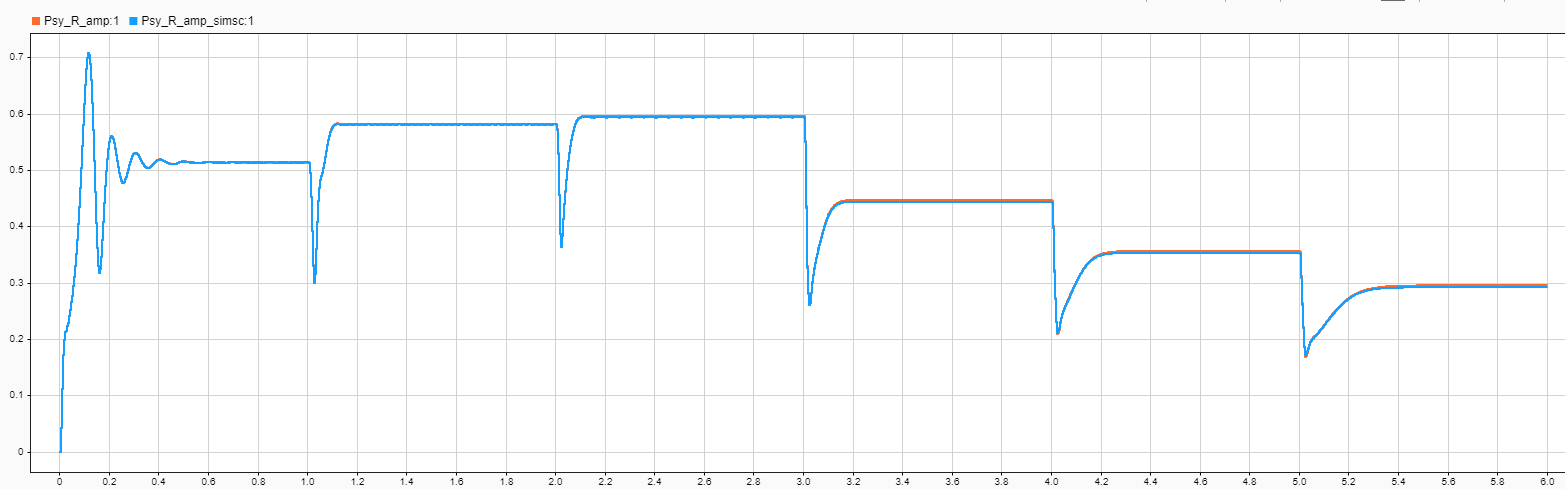
\includegraphics[width=14cm]{uf_flux}}
			\caption{ Rotorfluxus amplitúdó összehasonlítása}		
		\end{figure}
		
		\begin{figure}[!htb]
			\centering
			\label{uf_ang2}
			\tcbox{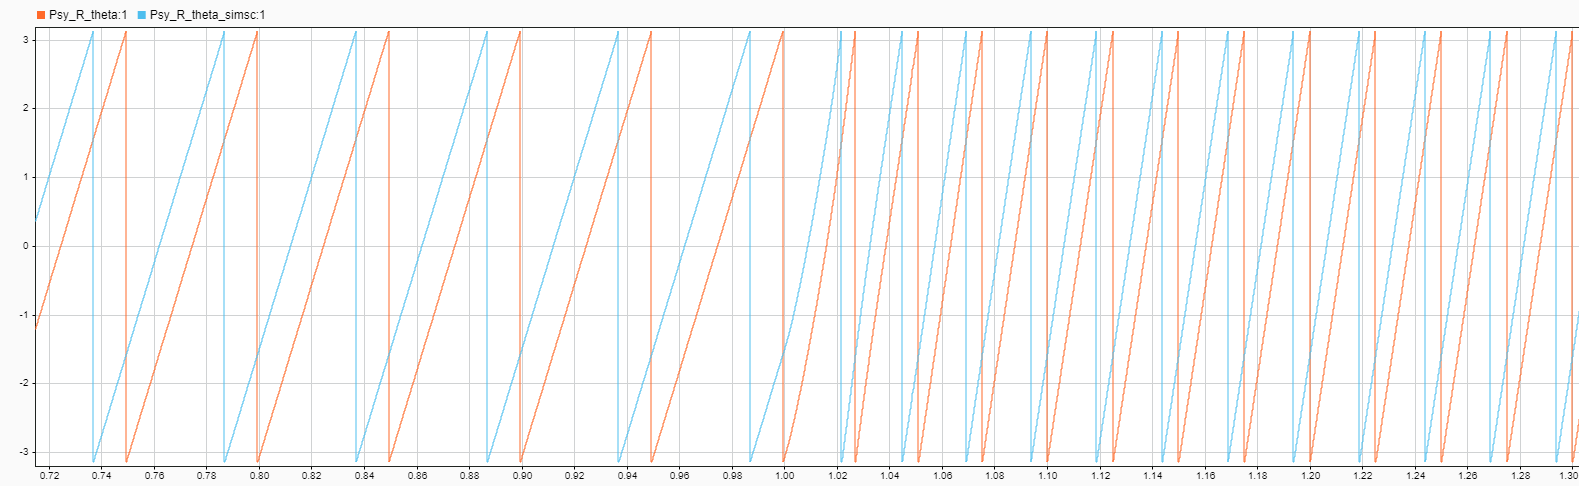
\includegraphics[width=14cm]{uf_ang2}}
			\caption{ Rotorfluxus szög összehasonlítása}		
		\end{figure}
		
		
		A (33) és (34) ábrát tanulmányozva jól látható, hogy mind a sebesség mint a fluxus, kisebb lengést követően beáll, a referencia értékre. A fluxus tekintetében megfigyelhető, hogy 60 Hz után csökken. Ez annak köszönhető ugyanis mezőgyengítési tartományban a fluxusképző komponens, vagyis a D irányú áram csökken. A rotorfluxus szög tekintetében egy 90 fokos eltérés van a mért és a számolt között, ez lényegében a D-Q koordináta-rendszer orientációjának tudható be, azonban mezőorientált szabályozásban ez nem lesz hatással a kontrollunkra.
		
		\begin{figure}[!htb]
			\centering
			\label{uf_duty}
			\tcbox{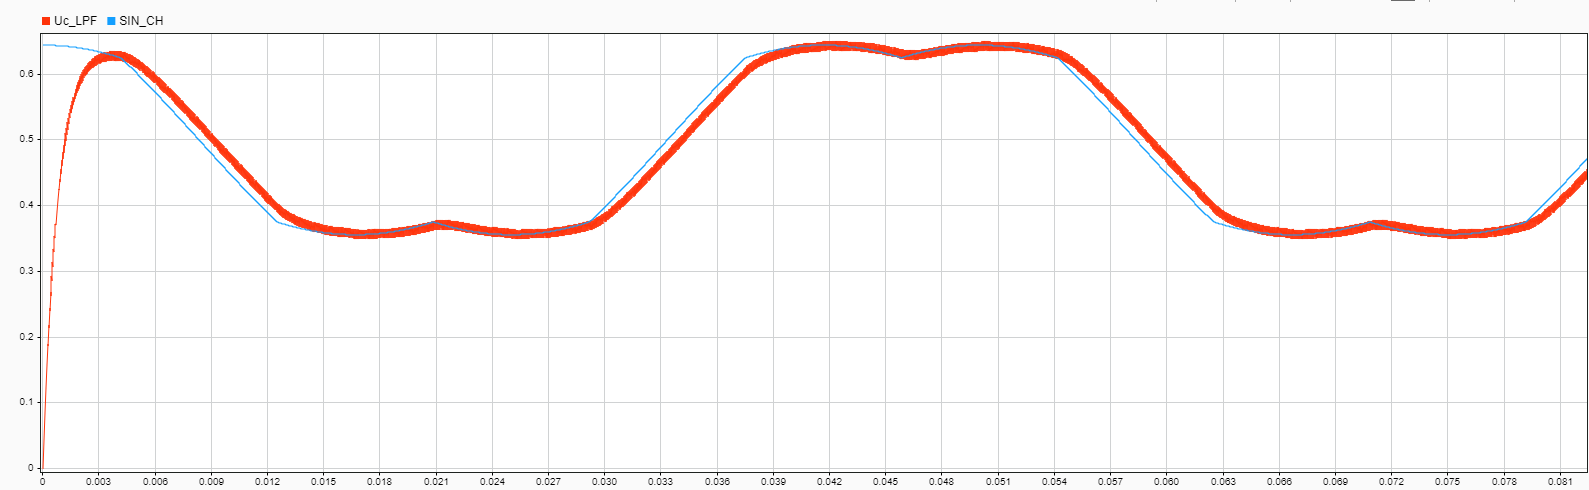
\includegraphics[width=14cm]{uf_duty}}
			\caption{ Kitöltési tényezők összehasonlítása}		
		\end{figure}
		
		Az invertervezérlés helyességét a kitöltési tényezők összehasonlításából tudjuk megállapítani. A (36) ábrán jól látható, hogy a referencia feszültségek frekvenciához méretezett IRR szűrő felhasználásával, a referencia kitöltésekkel jellegében megegyező kitöltéseket kapunk. A kitöltések frekvenciája és amplitúdója a szabályozás során, különböző szögsebességeken a fázisfeszültségekkel megegyezően változik. A sebességszabályozás tesztelése folyamán, szükséges a terhelőgép nyomatékának beállítása, hogy ne szálljon el a motor. Ha megnézzük a motor leadott nyomatékát, látható hogy az adott sebesség függvényében változik.
		\pagebreak
	\section{Tesztelés: Nyomatékszabályozás (FOC)}
	
	A bemutatott mezőorientált szabályozás komponenseinek, valamint a hardveres elemek összeépítéséből a választott motor függvényében paraméterezhető szimulációt kaptunk, amely alkalmas nyomatékszabályozásra. A szabályozás külső blokk vázlatán jól láthatóak, a visszacsatolásokat a motoron mért D - Q áramok és a rotorfluxus szög képezi.
	
	\begin{figure}[!htb]
		\centering
		\label{FOC}
		\tcbox{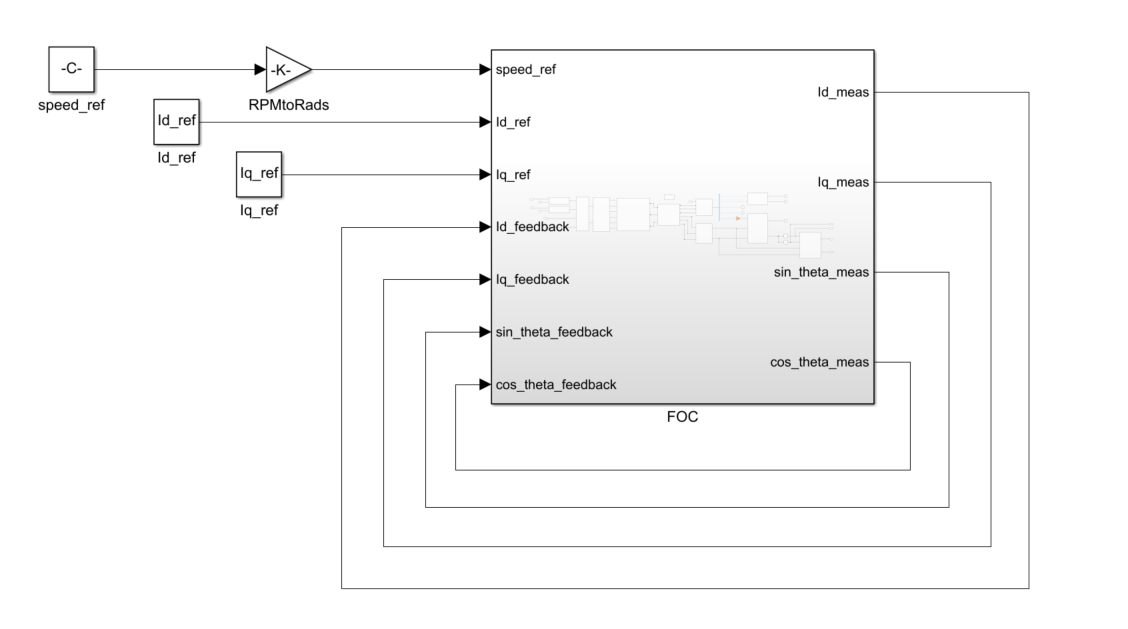
\includegraphics[width=14cm]{foc}}
		\caption{ FOC visszacsatolása}		
	\end{figure}
	
	A tesztelés során a modell működését statikus $L_m$-el, a főmező induktivitás szaturációja nélkül fogom bemutatni. Ahhoz hogy megfelelő képet kapjunk a szimulációról négy összehasonlító mérést kell végeznünk. Az első mérés során megvizsgáljuk hogy az áramszabályzókba motorról visszacsatolt áramok beállnak-e az mtpa által számolt referencia áramok értékére. Második körben szükséges megvizsgálni hogy a referencia áramokhoz előállításához szükséges feszültségek, tehát az áramszabályzók beavatkozó jelei állandósult állapotban, megfelelő toleranciák mellett, megegyeznek-e az mtpa által számolt értékekkel. Ehhez az adott munkapontban a D-Q irányú feszültségeket is eltároltam. Harmadik lépésben a szimuláció végén, feltételezve hogy a nyomaték állandósult, ennek megfelelően a rotorfluxus amplitúdónak is állandósulnia kell. Legutoljára pedig megnézzük, hogy a motoron generált nyomaték megegyezik-e a referenciával. A tesztelés elvégzéséhez az 50 Nm nyomaték megvalósításához szükséges munkapontot választottam ki, emellett a terhelőgép szögsebességét 1000 RPM-re állítottam. 
	
	\pagebreak
	\begin{figure}[!htb]
		\centering
		\label{mot_imp}
		\tcbox{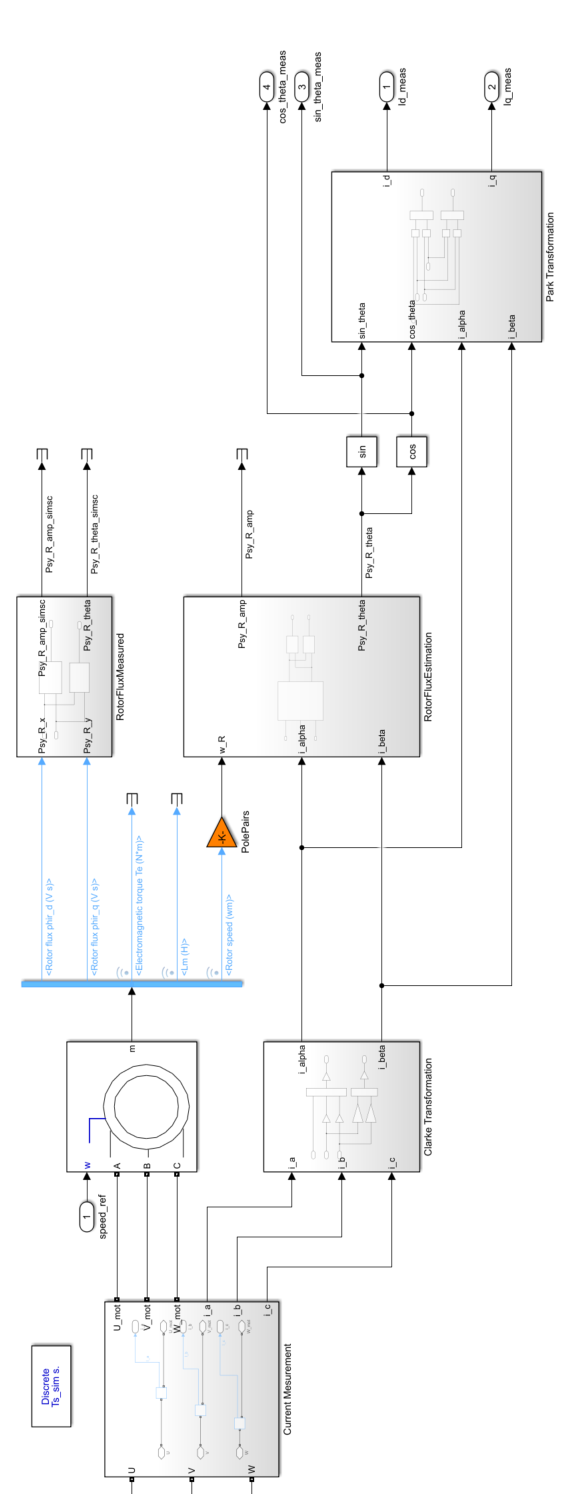
\includegraphics[width=8.1cm]{mot_imp}}
		\caption{Motor oldal implementációja }		
	\end{figure}
	\pagebreak
	\begin{figure}[!htb]
		\centering
		\label{inv_imp}
		\tcbox{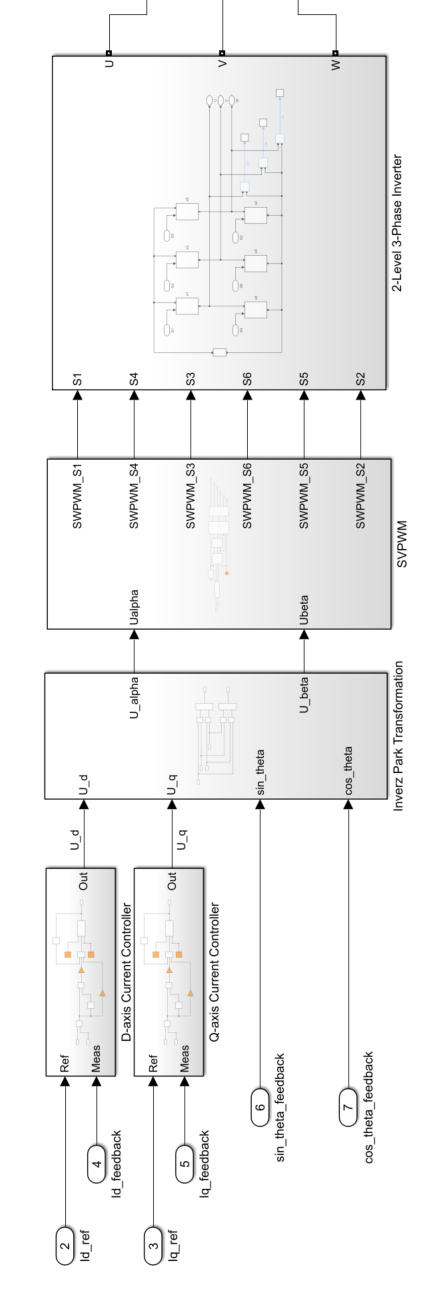
\includegraphics[width=7.1cm]{inv_imp}}
		\caption{ Inverter oldal implementációja}		
	\end{figure}
	

	\pagebreak
	
	\subsection{ Szimuláció paraméterei}
	\begin{flalign*}
		\\
		\rlap{\text{Munkapont referenciái:}} \\
		& Te = 50             && \text{ Nyomaték referencia [Nm]} \\
		& \omega_m = 1000     && \text{ Mechanikai szögsebesség [RPM]} \\
		\\
		\rlap{\text{A munkaponthoz tartozó MTPA által számolt referencia áram, feszültség és nyomaték értékei:}} \\
		\\
		& Te = 49.7562        && \text{ Számolt nyomaték referencia [Nm]} \\
		& i_{ds} = 23.6193    && \text{ D-irányú áramszabályzó referencia jele [A]} \\
		& i_{qs} = 22.9028    && \text{ Q-irányú áramszabályzó referencia jele [A]} \\
		& U_{ds} = -11.7981   && \text{ D-irányú beavatkozó jel [V]} \\
		& U_{qs} = 202.0248   && \text{ Q-irányú beavatkozó jel [V]} \\
		\\
		\rlap{\text{A felhasznált motor és inverter paraméterei:}} \\
		\\
		& U_{DC} = 400        && \text{ Egyenfeszültség forrás [V]} \\
		& R_s = 0.5968        && \text{ Stator oldali ellenállás [$\Omega$]} \\
		& R_r = 0.6258        && \text{ Rotor oldali ellenállás [$\Omega$]} \\
		& L_{ls} = 0.0003495  && \text{ Stator oldali szórási induktivitás [H]} \\
		& L_{lr} = 0.005473   && \text{ Rotor oldali szórási induktivitás [H]} \\
		& L_m = 0.0354        && \text{ Főmező induktivitás [H]} \\
		& p = 2               && \text{ Pólus párok száma [-]} \\
		& f_{nom} = 60        && \text{ Motor nominális frekvenciája [Hz]} \\
		& f_{samp} = 1000     && \text{ Impulzusszélességek mintavételi frekvenciája [Hz]} \\
		& f_{sw} = 20000      && \text{ Inverter kapcsolási frekvencia [Hz]} \\
		& Ts_{sim} = 1e-7     && \text{ Szimuláció/fizikai modellek solverének mintavételi ideje [s]} \\
		& K_p = 4             && \text{ Áramszabályzók P tagja [-]} \\
		& K_i = 1e-4          && \text{ Áramszabályzók I tagja [-]} \\
		& U_{min} = -U_{DC} \ \sqrt{3} && \text{ Áramszabályzók szaturációjának minimum limitje [V]} \\
		& U_{max} =  U_{DC} \ \sqrt{3} && \text{ Áramszabályzók szaturációjának maximum limitje [V]}
	\end{flalign*}
	

	\subsection{ Mérések }
	\hfill\break
	\begin{figure}[!htb]
		\centering
		\label{ids}
		\tcbox{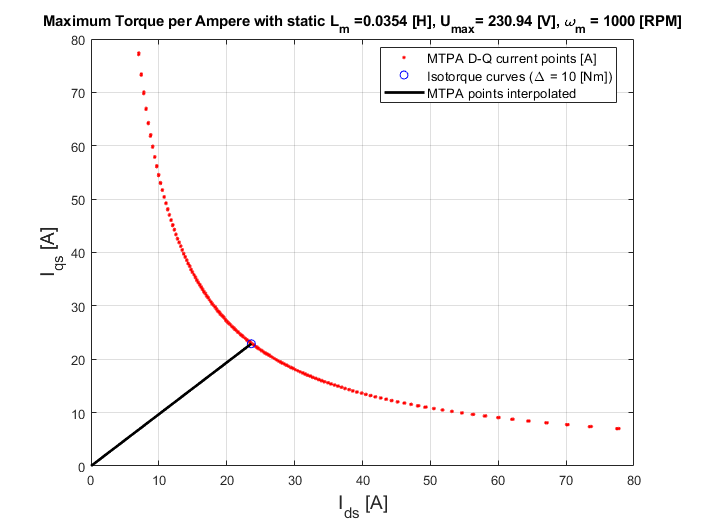
\includegraphics[width=14cm]{lm}}
		\caption{ Munkapont nyomatékgörbéje}		
	\end{figure}
	
	Az (40)-as ábra ábrázolja a referencia nyomatékhoz tartozó nyomatékgörbét az áramok függvényében, valamint a kiválasztott munkapont megvalósításához szükséges legoptimálisabb áramokat.
	
	\pagebreak
	\begin{figure}[!htb]
		\centering
		\label{ids}
		\tcbox{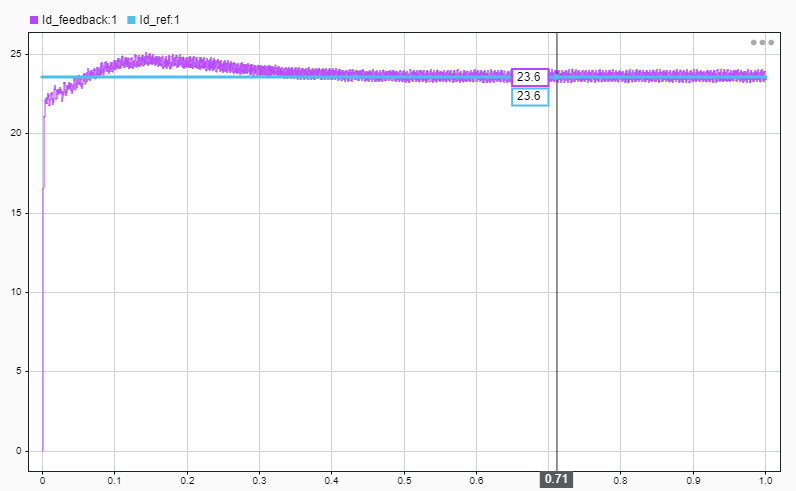
\includegraphics[width=12cm]{ids}}
		\caption{Referencia és mért D-áram összehasonlítása}		
	\end{figure}
	\begin{figure}[!htb]
		\centering
		\label{iqs}
		\tcbox{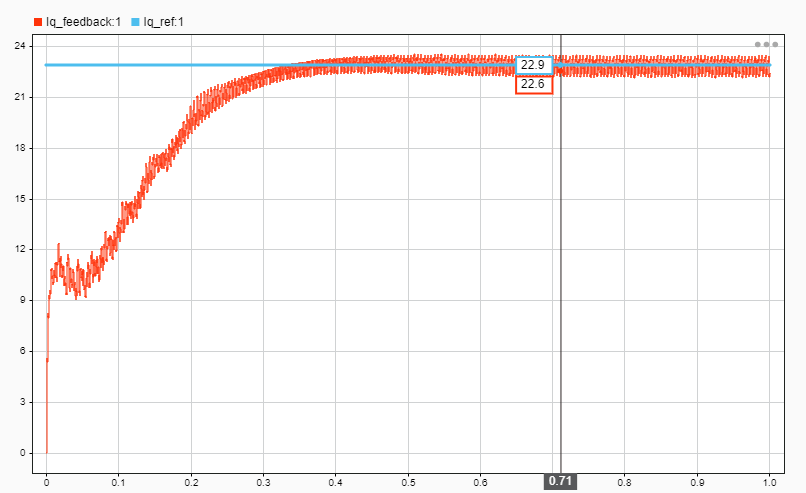
\includegraphics[width=12cm]{iqs}}
		\caption{Referencia és mért Q-áram összehasonlítása}		
	\end{figure}
	A (41) és (42)-es ábrán jól látszik, hogy a motorról visszacsatolt áramok, a D - irány tekintetében kis túllövés után jól beállnak az MTPA által számolt referenciára. Emellett, ha megfigyeljük a (45)-as ábrát, amely a rotorfluxust ábrázolja észrevehető, hogy jellegében hasonló a D - irányú áramhoz, ha pedig a (46)-es ábrát vizsgáljuk ugyanezen hasonlóság fedezhető fel a motor nyomatéka, valamint a Q - irányú áram között. Ezáltal mérések is igazolják, hogy a D - irányú áram a fluxusképző, a Q - irányú áram a nyomatékképző komponensnek feleltethető meg.
	\pagebreak
	
	\begin{figure}[!htb]
		\centering
		\label{uds}
		\tcbox{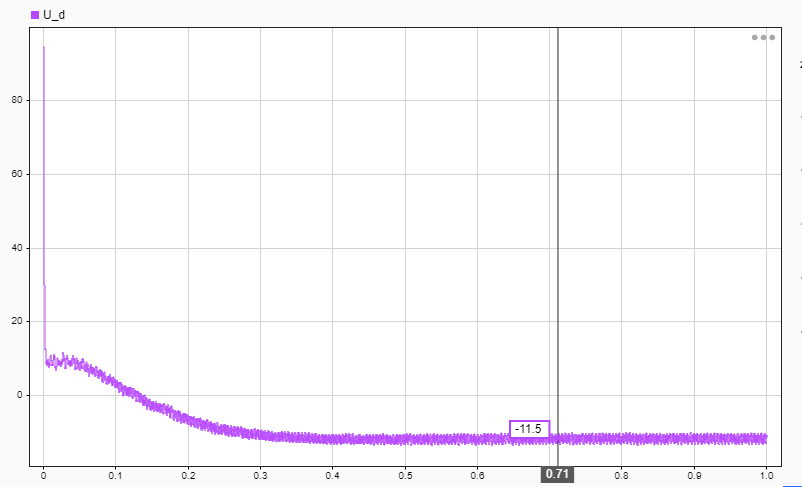
\includegraphics[width=12cm]{uds}}
		\caption{D-irányú feszültség mérése}		
	\end{figure}
	\begin{figure}[!htb]
		\centering
		\label{uqs}
		\tcbox{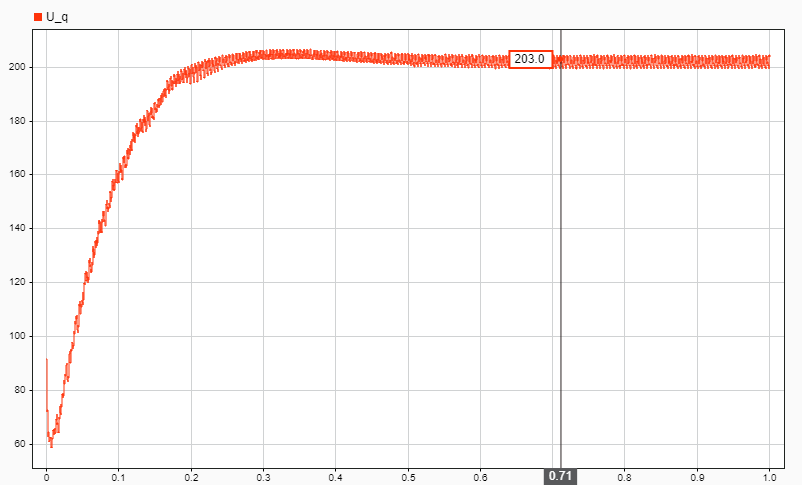
\includegraphics[width=12cm]{uqs}}
		\caption{Q-irányú feszültség mérése}		
	\end{figure}
	A (43) és (44)-es ábrán látható hogy ezek is beállnak az MTPA által számolt értékekre, ezzel bizonyítva hogy jól számoltuk az áramok előállításához szükséges feszültségeket.
	\pagebreak
	
	\begin{figure}[!htb]
		\centering
		\label{flux}
		\tcbox{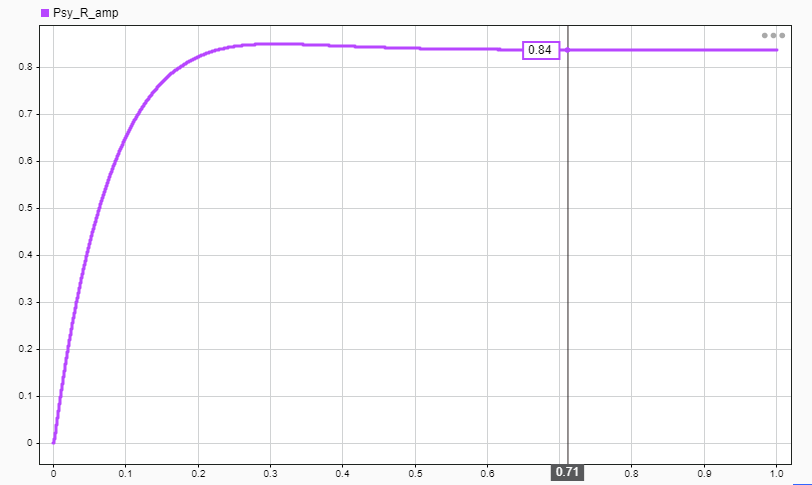
\includegraphics[width=12cm]{flux}}
		\caption{ Rotorfluxus mérése}		
	\end{figure}
		\begin{figure}[!htb]
		\centering
		\label{Te}
		\tcbox{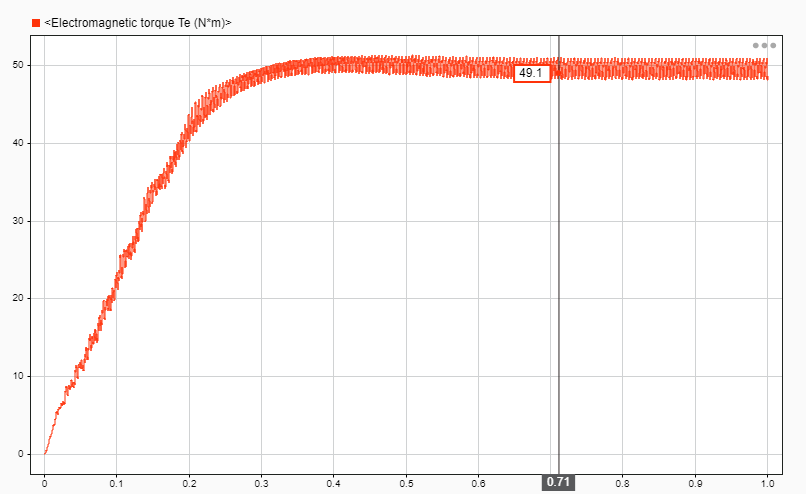
\includegraphics[width=12cm]{Te}}
		\caption{ Motor nyomatékának mérése}		
	\end{figure}
	
	A (46)-es ábra tekintetében látható, hogy a nyomaték kellő pontossággal beáll az 50 Nm-es értékre. A (45)-as ábrán jól látható hogy állandó nyomaték esetén, nem történik fluxus változás állandósult állapotban ( ez a stator fluxusokra is igaz) és a nyomaték beállásával a fluxus is állandósul.
	
	
	\pagebreak
	\hfill\break
	A fentebbi ábrákon jól látszik, hogy az elvárásoknak megfelelően, minden pontban teljesítik a fent leírtakat, ugyanis a szükséges mérések beállnak a referencia értékre és a kialakult nyomaték is megegyezik az elvárttal.
	
	Az induktivitás szaturációjának számbavételével, a nyomaték hasonlóan állandósul, de viszonylag nagy eltérés tapasztalható a referencia nyomaték és az állandósult állapot között. Ez főként abból adódik, hogy a felhasznált Simscapes motormodell másképp számolja a főmező induktivitás telítődését.
	
	A munkaponthoz tartozó MTPA által számolt referencia áram, feszültség és nyomaték értékei a főmező induktivitás mágneses telítődés beleszámolásával:
	\begin{flalign*}
		& Te = 49.8317        && \text{ Számolt nyomaték referencia [Nm]} \\
		& i_{ds} = 25.5790    && \text{ D-irányú áramszabályzó referencia jele [A]} \\
		& i_{qs} = 36.5359    && \text{ Q-irányú áramszabályzó referencia jele [A]} \\
		& U_{ds} = -26.2544   && \text{ D-irányú beavatkozó jel [V]} \\
		& U_{qs} = 160.1408   && \text{ Q-irányú beavatkozó jel [V]} 
	\end{flalign*}
	
	\begin{figure}[!htb]
		\centering
		\label{ids}
		\tcbox{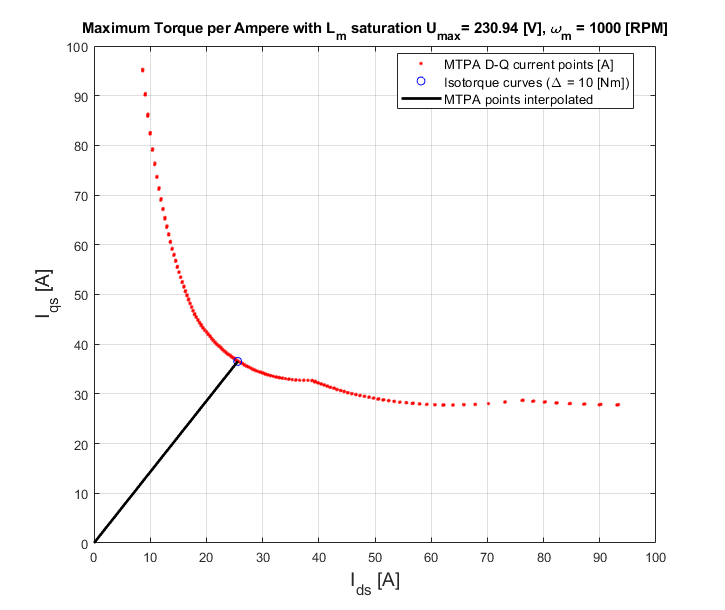
\includegraphics[width=12cm]{lm_sat}}
		\caption{ Munkapont nyomatékgörbéje telítődés beleszámolásával}		
	\end{figure}
	
	\begin{figure}[!htb]
		\centering
		\label{Te}
		\tcbox{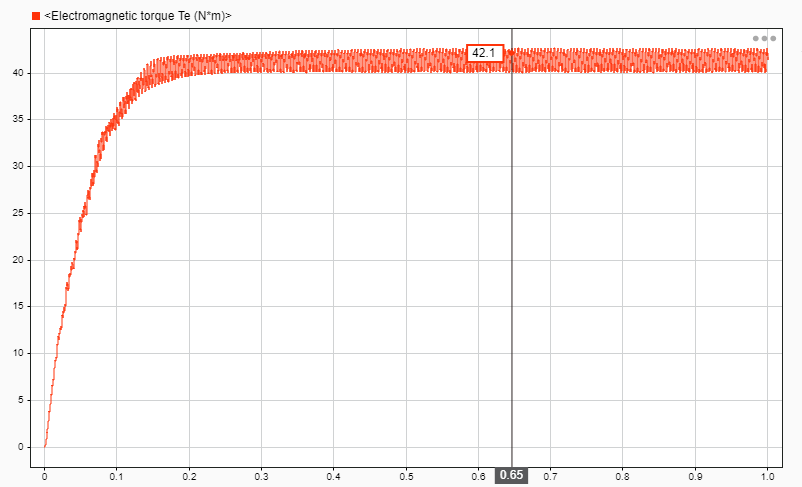
\includegraphics[width=14cm]{Te_sat}}
		\caption{ Motor nyomatéka mágneses telítődés beleszámolásával}		
	\end{figure}
	
	\section{Összegzés és továbbfejlesztési lehetőségek}
	
	Ahogy a mérésekből is látszik, szimulációs környezetben a szabályozás működik, ha a főmező induktivitást statikusnak vesszük. A modell tartalmazza a mezőorientált szabályozáshoz szükséges hajtásvezérlés elemeit. Tovább fejlesztés tekintetében első körben a főmező induktivitás telítődésének számítását kellene újra gondolni, akár fluxusból számolni, ahogy azt a motor modell is teszi. A fő cél a hardveres implementálás volna, ahol bővíthetném tudásomat a mikrokontrollerek programozásában és a szimulációt átlépve a valóságban lehetne mérni a motor hatékonyságát. A szoftver tekintetében a hardveres megvalósítás új komponensek készítését is magával vonná, például a PWM jelekhez tartozó holtidő kompenzáció tervezése, valamint az áramszabályzók motor modell alapú kalibrációja.
	
	\pagebreak
	\section{Glossary}
	
	As the measurements show in the simulation environment, the control works when considering the main field inductance as static. The model includes the necessary drive control elements  for field-oriented control. For further development, the calculation of the saturation of the main field inductance should be reconsidered, possibly calculating it from flux, as the motor model also does. The main goal would be the hardware implementation, where I could expand my knowledge in microcontroller programming, and beyond simulation, measure the efficiency of the motor in real-world scenarios. Regarding software, the hardware implementation would involve creating new components, such as designing dead-time compensation for PWM signals and calibrating current regulators based on the motor model.
	
	
		\pagebreak
		\nomenclature{\(U_{i}\)}{indukált feszültség \hfill V}
		\nomenclature{\(U_{DC}\)}{ DC feszültség \hfill V}
		\nomenclature{\(X\)}{Impedancia \hfill $\Omega$}
		\nomenclature{\(U_{nom}\)}{ Nominális feszültség \hfill V}
		\nomenclature{\(p\)}{ Pólus párok száma \hfill -}
		\nomenclature{\({\omega}\)}{ Állórész szögsebesség (szinkron sebesség) \hfill rad/s}
		\nomenclature{\({\omega_r}\)}{ Rotor elektrikus szögsebessége \hfill rad/s}
		\nomenclature{\({\omega_m}\)}{ Mechanikai szögsebesség \hfill rad/s}
		\nomenclature{\({\omega_{slip}}\)}{ Slip szögsebesség \hfill rad/s}
		\nomenclature{\({\omega_{rated}}\)}{ Nominális szögsebesség \hfill rad/s}
		\nomenclature{\(R_s\)}{ Stator oldali ellenállás\hfill $\Omega$ }
		\nomenclature{\(R_r\)}{ Rotor oldali ellenállás\hfill $\Omega$ }
		\nomenclature{\(\Psi_{ds}\)}{D - irányú stator fluxus \hfill Wb}
		\nomenclature{\(\Psi_{qs}\)}{Q - irányú stator fluxus \hfill Wb}
		\nomenclature{\(\Psi_{dr}\)}{D - irányú rotor fluxus \hfill Wb}
		\nomenclature{\(\Psi_{qr}\)}{Q - irányú rotor fluxus \hfill Wb}
		\nomenclature{\(\Psi_{r\alpha}\)}{Alpha - irányú rotor fluxus \hfill Wb}
		\nomenclature{\(\Psi_{r\beta}\)}{Beta - irányú rotor fluxus \hfill Wb}
		\nomenclature{\(\Theta_{\Psi_r}\)}{Rotor fluxus szög \hfill rad/s}
		\nomenclature{\(L_{s}\)}{ Stator induktivitás \hfill H}
		\nomenclature{\(L_{r}\)}{ Rotor induktivitás \hfill H}
		\nomenclature{\(L_{ls}\)}{ Stator szórási induktivitás \hfill H}
		\nomenclature{\(L_{lr}\)}{ Rotor szórási induktivitás \hfill H}
		\nomenclature{\(L_{m}\)}{ Főmező induktivitás \hfill H}
		\nomenclature{\(\Psi_{M}\)}{ Főmező fluxus \hfill Wb}
		\nomenclature{\(i_{dr}\)}{D - irányú rotor áram \hfill A}
		\nomenclature{\(i_{qr}\)}{Q - irányú rotor áram \hfill A}
		\nomenclature{\(i_{ds}\)}{D - irányú stator áram \hfill A}
		\nomenclature{\(i_{qs}\)}{Q - irányú stator áram \hfill A}
		\nomenclature{\(i_{r\alpha}\)}{Alpha - irányú rotor áram \hfill A}
		\nomenclature{\(i_{r\beta}\)}{Beta - irányú rotor áram \hfill A}
		\nomenclature{\(i_{s\alpha}\)}{Alpha - irányú stator áram \hfill A}
		\nomenclature{\(i_{s\beta}\)}{Beta - irányú stator áram \hfill A}
		\nomenclature{\(i_{m}\)}{Mágnesező áram \hfill A}
		\nomenclature{\(U_{ds}\)}{D - irányú stator feszültség \hfill V}
		\nomenclature{\(U_{qs}\)}{Q - irányú stator feszültség \hfill V}
		\nomenclature{\(U_{dr}\)}{D - irányú rotor feszültség \hfill V}
		\nomenclature{\(U_{qr}\)}{Q - irányú rotor feszültség \hfill V}
		\nomenclature{\(\vec{U}_{s}\)}{ Stator feszültség vektor \hfill V}
		\nomenclature{\(\vec{U}_{svec}\)}{ Térvektor \hfill V}
		\nomenclature{\(m\)}{ Modulációs index \hfill -}
		\nomenclature{\(\vec{U}_{ref}\)}{ Referencia feszültség vektor \hfill V}
		\nomenclature{\(T_{r}\)}{ Rotor időállandója \hfill -}
		\nomenclature{\(T_{1}, T_{2}\)}{ Aktív vektorok impulzusszélességei  \hfill -}
		\nomenclature{\(T_{s}\)}{ Szimuláció mintavételi ideje  \hfill -}
		\nomenclature{\(\alpha\)}{Szűrő együttható \hfill -}
		\nomenclature{\(C\)}{Kapacitás \hfill F}
		\nomenclature{\(f_{c}\)}{ Vágási frekvencia \hfill Hz}
		\nomenclature{\(\omega_{c}\)}{ Vágási körfrekvencia \hfill rad/s}
		\nomenclature{\(f_{fund}\)}{ Alapharmónikus frekvencia \hfill Hz}
		\nomenclature{\(Te\)}{Forgatónyomaték \hfill Nm}
		\nomenclature{\(\vec{I}_s\)}{Stator áram vektor \hfill A}
		\nomenclature{\(U_U\)}{U fázis fázisfeszültsége \hfill V}
		\nomenclature{\(U_V\)}{V fázis fázisfeszültsége \hfill V}
		\nomenclature{\(U_W\)}{W fázis fázisfeszültsége \hfill V}
		
		
		\printnomenclature
		\pagebreak
	
	\section{Mellékletek}
		\begin{appendix}
			\listoffigures
		\end{appendix}
		\pagebreak
	\section{Irodalomjegyzék}
	
		\nocite{*}
		\bibliographystyle{plain}  % Choose your bibliography style
		\bibliography{lib}   % Specify the name of your BibTeX file without 
	
	
\end{document}